%
% Master thesis template for Ghent University (2018)
%
%
%  !!!!!!!!!!!!!!!!!!!!!!!!!!!!!!!!!!!!!!!!!!!!!!!!!!!!!!!!!!!!
%  !!  MAKE SURE TO SET lualatex OR xelatex AS LATEX ENGINE  !!
%  !!!!!!!!!!!!!!!!!!!!!!!!!!!!!!!!!!!!!!!!!!!!!!!!!!!!!!!!!!!!
%  !! For overleaf:                                          !!
%  !!     1. click gear icon in top right                    !!
%  !!     2. select `lualatex` in "latex engine"             !!
%  !!     3. click "save project settings"                   !!
%  !!                                                        !!
%  !!!!!!!!!!!!!!!!!!!!!!!!!!!!!!!!!!!!!!!!!!!!!!!!!!!!!!!!!!!!
%
%
%  History
%    2014         Doctoral Thesis of Bruno Volckaert
%    2017         Adapted to master thesis by Jerico Moeyersons
%    2018         Cleanup by Merlijn Sebrechts
%
%  Latest version
%    https://github.com/galgalesh/masterproef-template
%
\documentclass[11pt,a4paper,twoside, openany]{book}
\usepackage[a4paper,includeheadfoot,margin=2.50cm]{geometry}

\setlength{\parindent}{0cm}           % indent of the first sentence of a paragraph
\setlength{\parskip}{1em}             % space between paragraphs
\renewcommand{\baselinestretch}{1.2}  % stretch horizontal space between everything

\usepackage{graphicx}
\graphicspath{{images/}}
\usepackage{pdfpages}
\usepackage{enumitem}
\usepackage{float}
\usepackage{caption}
\usepackage{subcaption}
\usepackage[toc,page]{appendix}
\usepackage[section]{placeins}
\makeatletter
\AtBeginDocument{%
	\expandafter\renewcommand\expandafter\subsection\expandafter{%
		\expandafter\@fb@secFB\subsection
	}%
}
\makeatother
\usepackage{svg}
\usepackage{amsmath}
\usepackage{graphicx}
\usepackage{epstopdf}
\epstopdfsetup{update} % only regenerate pdf files when eps file is newer

\usepackage[chapter]{minted}                           % for modern code highlighting
\newenvironment{code}{\captionsetup{type=listing}}{}   % To get multiline code fragments working: https://tex.stackexchange.com/a/53540/72273

\AtBeginEnvironment{minted}{\fontsize{9}{9}\selectfont}

\PassOptionsToPackage{hyphens}{url}
\usepackage{hyperref}
\usepackage{url}

\usepackage{quotchap}              % For the fancy quotes next to the chapter titles

\usepackage[numbers]{natbib}       % For bibliography; use numeric citations
\bibliographystyle{IEEEtran}
\usepackage[nottoc]{tocbibind}     % Put Bibliography in ToC

%
% Defines \checkmark to draw a checkmark
%
\usepackage{tikz}
\def\checkmark{\tikz\fill[scale=0.4](0,.35) -- (.25,0) -- (1,.7) -- (.25,.15) -- cycle;}

%
% For tables
%
\usepackage{booktabs}
\usepackage{array}
\usepackage{ragged2e}  % for '\RaggedRight' macro (allows hyphenation)
\newcolumntype{L}[1]{>{\raggedright\let\newline\\\arraybackslash\hspace{0pt}}m{#1}}
\newcolumntype{C}[1]{>{\centering\let\newline\\\arraybackslash\hspace{0pt}}m{#1}}
\newcolumntype{R}[1]{>{\raggedleft\let\newline\\\arraybackslash\hspace{0pt}}m{#1}}

%
% Support for splitting Dutch words correctly
%
\usepackage{polyglossia}
\setdefaultlanguage[babelshorthands=true]{dutch}

% Manually specify additional hypnations for words
\hyphenation{Linked Connections LC2Irail}

%
% Translated strings. If these aren't set, the English words are used.
%
\addto\captionsenglish{%
  \renewcommand{\contentsname}%
    {Inhoudsopgave}%
}
\renewcommand\appendixtocname{Bijlagen}
\renewcommand\appendixpagename{Bijlagen}
\renewcommand{\listoflistingscaption}{Lijst van listings}

\newfloat{code}{thp}{lop}
\floatname{code}{Code}

\newcommand\foreign[1]{\emph{#1}}
\newcommand\inlinecode[1]{\emph{#1}}
%
% Set the title and your name
%
\title{The user perceived performance of route planning APIs}
\author{Bert Marcelis}

%
%  END OF HEADER
%  The actual latex document content starts here.
%
\begin{document}

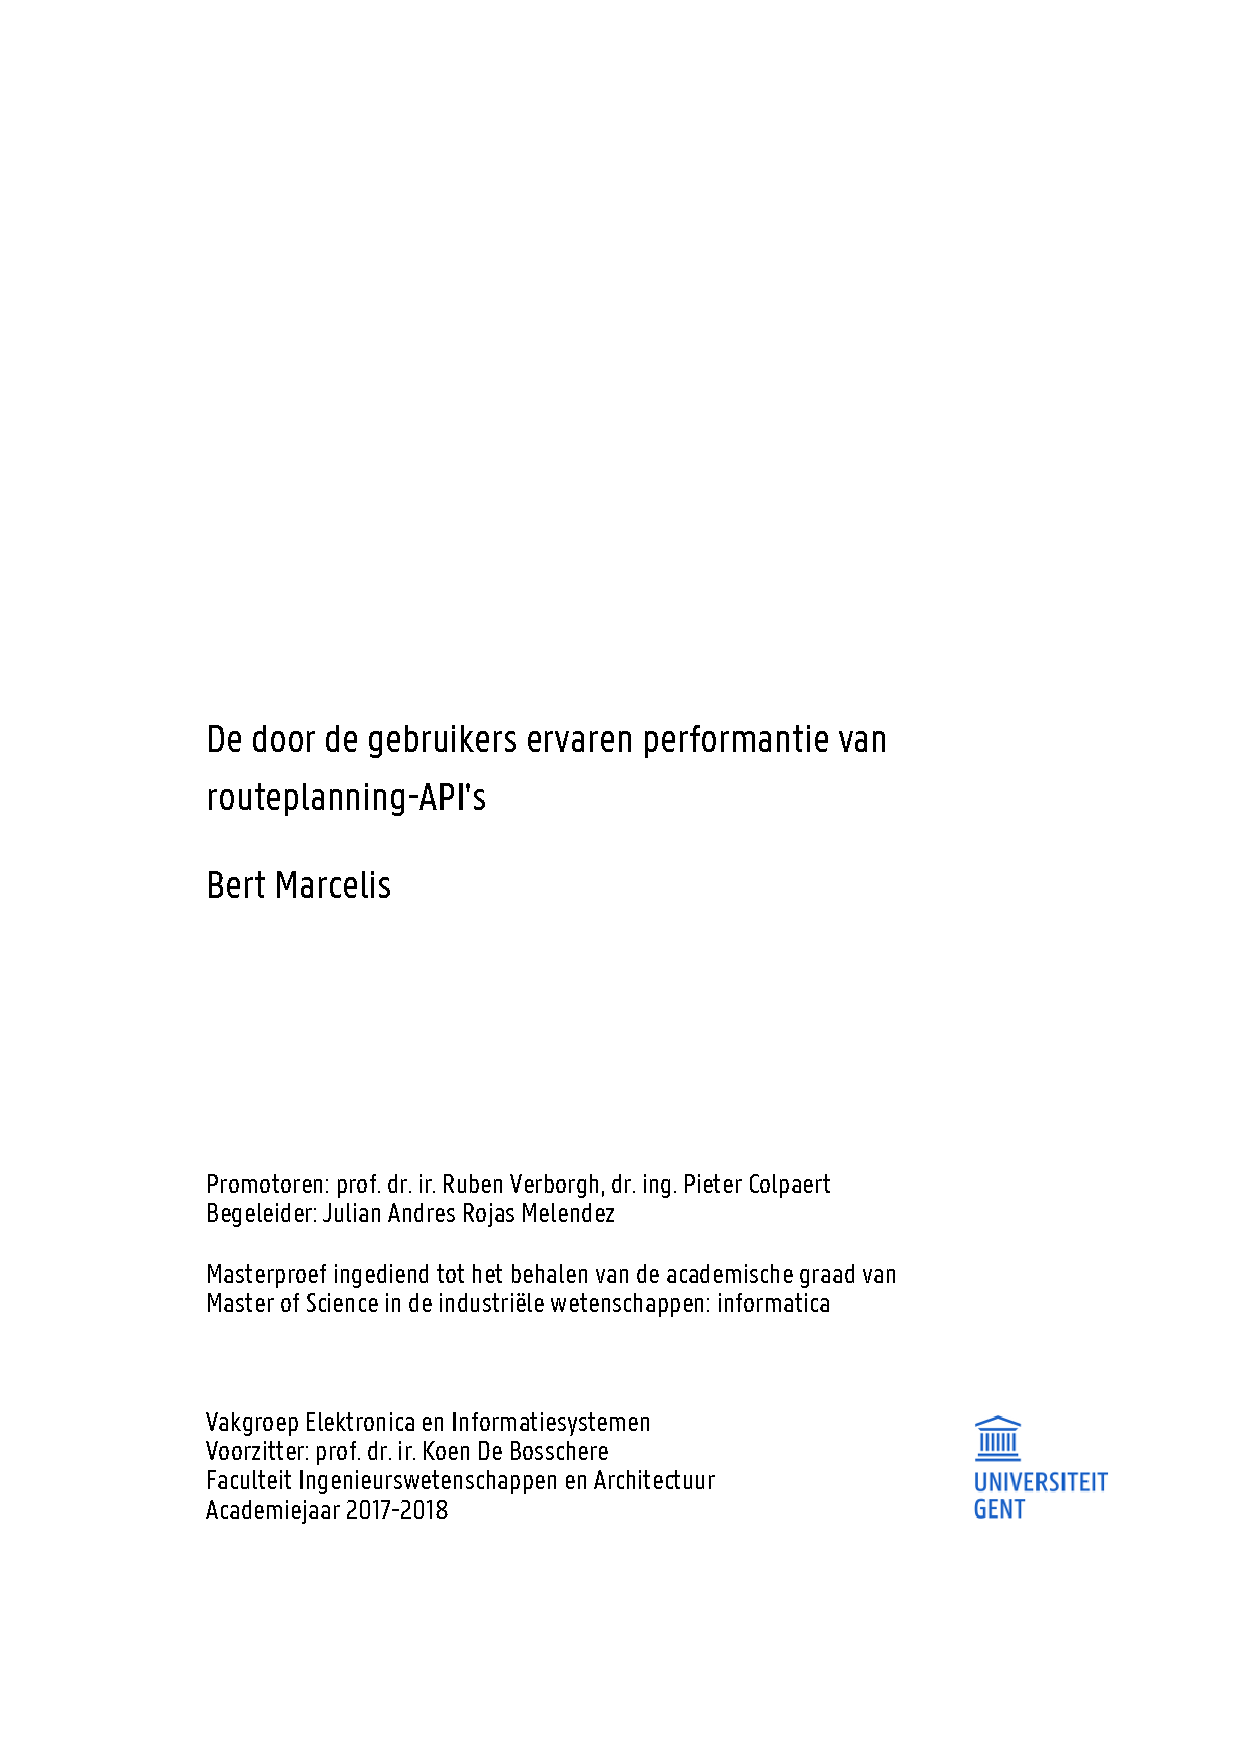
\includepdf{voorblad.pdf}             % Front matter
\newpage\thispagestyle{empty}\mbox{}  % White page
% !TeX spellcheck = nl_NL
\thispagestyle{empty}    % Don't show page number
\begin{center}
\textbf{Dankwoord}
\end{center}

Na zes maanden zwoegen is deze masterproef eindelijk klaar. Hoewel ik dit werk zelf moest maken, zou dit niet mogelijk geweest zijn zonder de hulp van een aantal mensen rondom mij. 

Als eerste wil ik mijn promotor Pieter Colpaert bedanken. Pieter, zonder jouw continue begeleiding, feedback, en talloze uren aan nalezen zou ik dit werk nooit tot een goed einde hebben gebracht. Ik wil ook mijn begeleider Julian Melendez bedanken, voor de hulp bij het verder ontwikkelen van Linked Connections en het nalezen van mijn scriptie.

Daarnaast wil ik ook graag mijn ouders bedanken, voor de steun en om altijd klaar te staan als ik hulp nodig had en te zorgen dat ik na een week hard werken steeds in een warm nest kon thuiskomen. Ik wil ook mijn vriendin Sofie bedanken voor de steun, de aanmoediging en het geduld doorheen deze maanden van hard werk. Ook mijn vrienden wil ik hier niet vergeten, die steeds voor wat ontspanning konden zorgen tussen de schrijf- of werksessies in.

Tot slot wens ik iedereen te bedanken die heeft bijgedragen aan het onderzoek, door deel te nemen aan de user-testing, door de enquête in te vullen, of door mee te helpen bij het verspreiden van de enquête.

Bedankt iedereen!

Bert Marcelis
          % Word of thanks
\newpage\thispagestyle{empty}\mbox{}  % White page
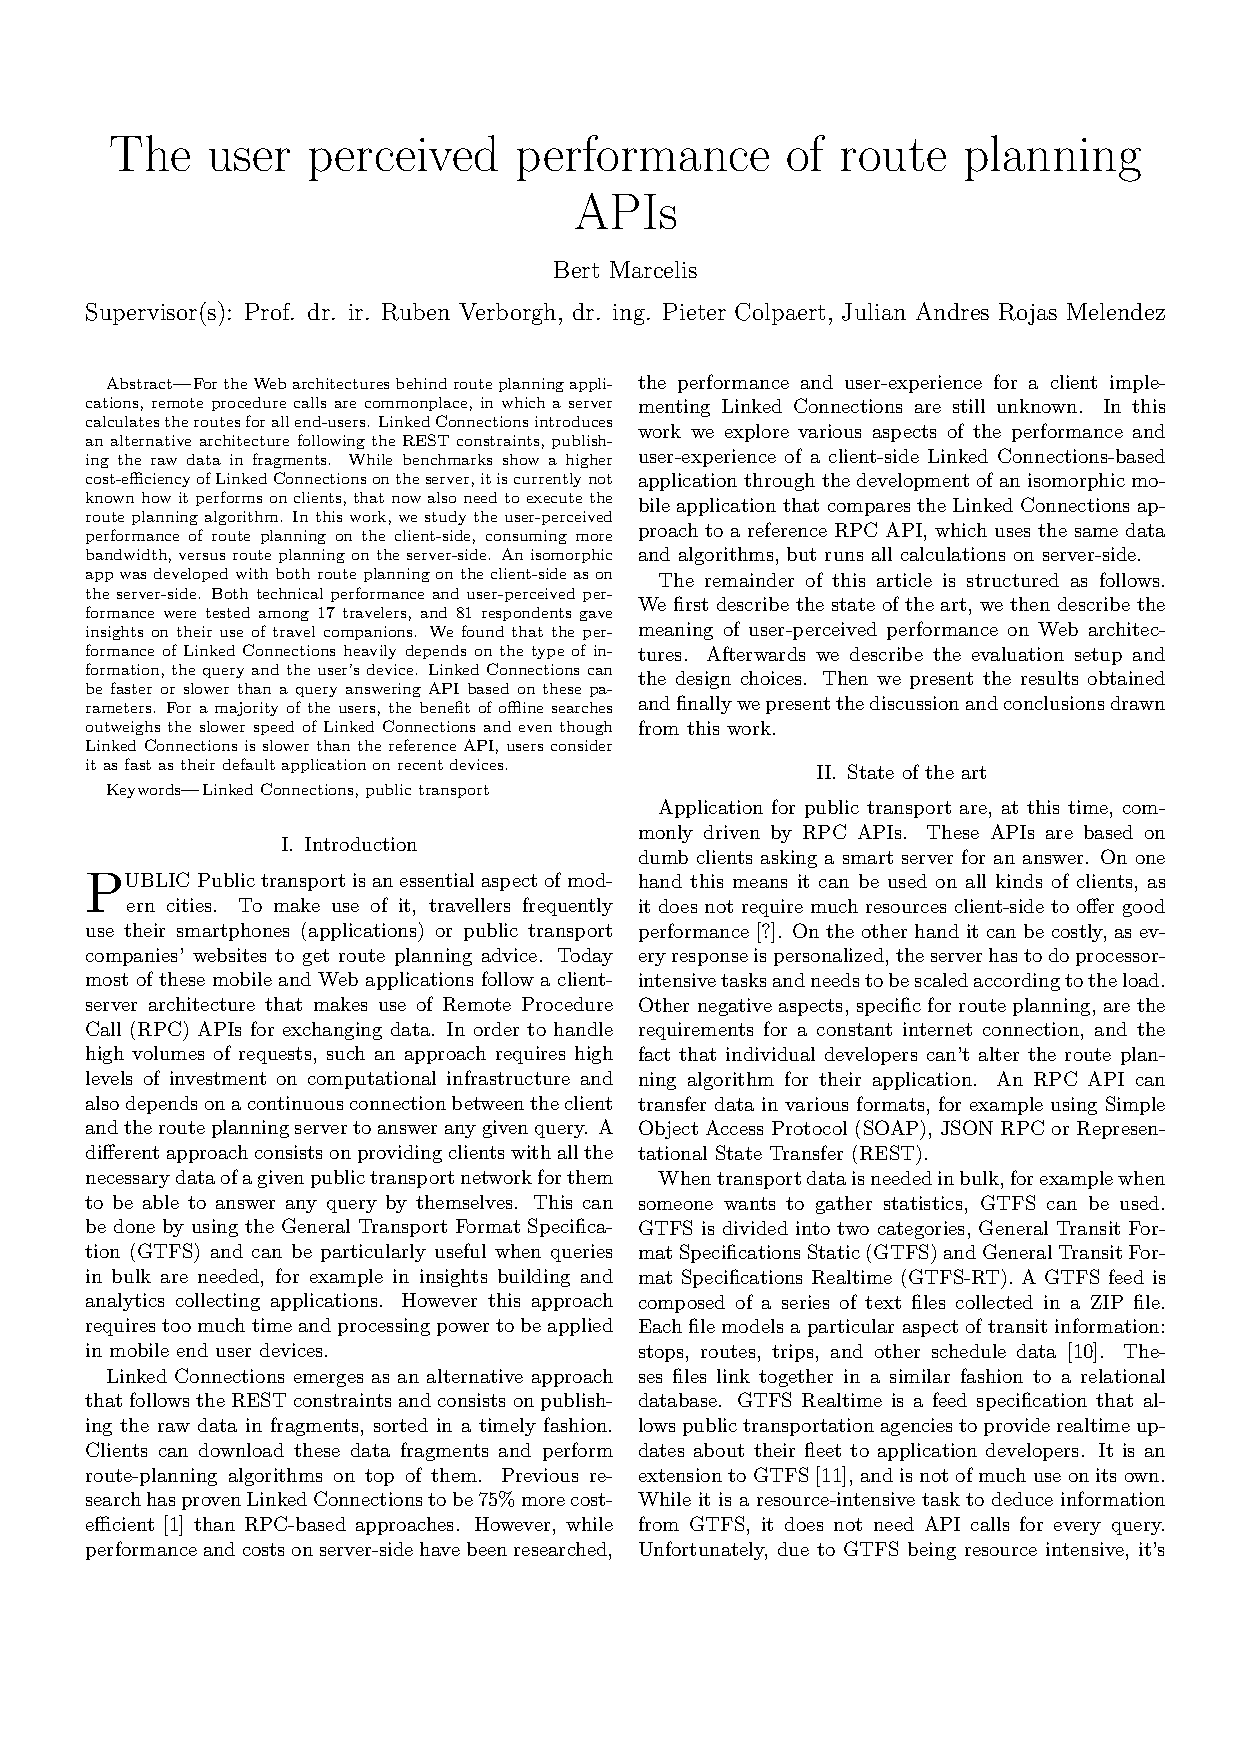
\includepdf[pages={-}]{abstract.pdf}  % Extended Abstract
\tableofcontents                      % Table of Contents
\listoffigures                        % List of figures
\listoftables                         % List of tables
\listoflistings                       % List of listings (code fragments)

%
% Include the main chapters of the thesis below
%

% https://twitter.com/Stwaf/status/989531577947492358

\begin{savequote}[0.55\linewidth]
	``Inspirational quote''
	\qauthor{\textasciitilde Source}
\end{savequote}

\chapter{Inleiding}
\label{chap:intro}
Openbaar vervoer is ook een essentiële dienst in elke stad\citep{programmableweb14}. Om vlot van dit openbaar vervoer gebruik te maken, zijn er tientallen websites en apps (user-agents) die gebruikers informatie verstrekken over vertrekken, aankomsten, ritten, routes en vertragingen. Voorbeelden hiervan in België zijn iRail.be, HyperRail en Railer, en CityMapper, TheTransitApp, Here WeGo en Google maps wereldwijd. Op dit moment zijn al deze user-agents echter toegewezen op het gebruik van data dumps of specifieke APIs om informatie met betrekking tot openbaar vervoer te publiceren, of een variant ervan. 

Enerzijds zijn er volledige data dumps, in de vorm van General Transit Feed Specification (GTFS)\footnote{https://developers.google.com/transit/gtfs/} en General Transit Feed Specification Realtime (GTFS-RT)\footnote{https://developers.google.com/transit/gtfs-realtime/}. GTFS bestanden bevatten informatie over alle voertuigen van een dienstverlener, over een relatief grote tijdspanne, typisch enkele maanden tot een jaar. GTFS-RT bestanden bevatten realtime informatie over ritten in de komende dag. Om al deze data compact op te slaan en te versturen, worden deze opgeslagen in de vorm van regels. Deze regels omschrijven wanneer welk voertuig welke rit maakt. Om op basis van deze regels vragen te beantwoorden, dient deze set abstracte regels omgevormd te worden naar een gepast model waarin ritten en stopplaatsen opgevraagd kunnen worden, en routes berekend kunnen worden. Hiervoor zijn, afhankelijk van welke informatie gewenst is, zware berekeningen vereist, die afhankelijk van de grootte van het GTFS bestand vijf à tien minuten kunnen duren op een moderne computer. Gebruikers kunnen geen 10 minuten wachten tot de data getransformeerd zijn, waardoor deze optie niet beschikbaar is op mobiele toestellen. Verder is dit formaat een mogelijke technologische restrictie op de vervoersdata: enkel gevorderde ontwikkelaars kunnen hiervan gebruik maken. Open data is slechts open als deze (onder andere) beschikbaar zijn in een begrijpbaar formaat~\citep{okfn18}. GTFS is dus vooral geschikt om vervoersdata te delen met grote bedrijven, en in mindere mate voor individuele ontwikkelaars die vervoers data eenvoudig willen visualiseren (digital signage, routeplanner applicaties, websites, ...).

\begin{figure}
	\centering
	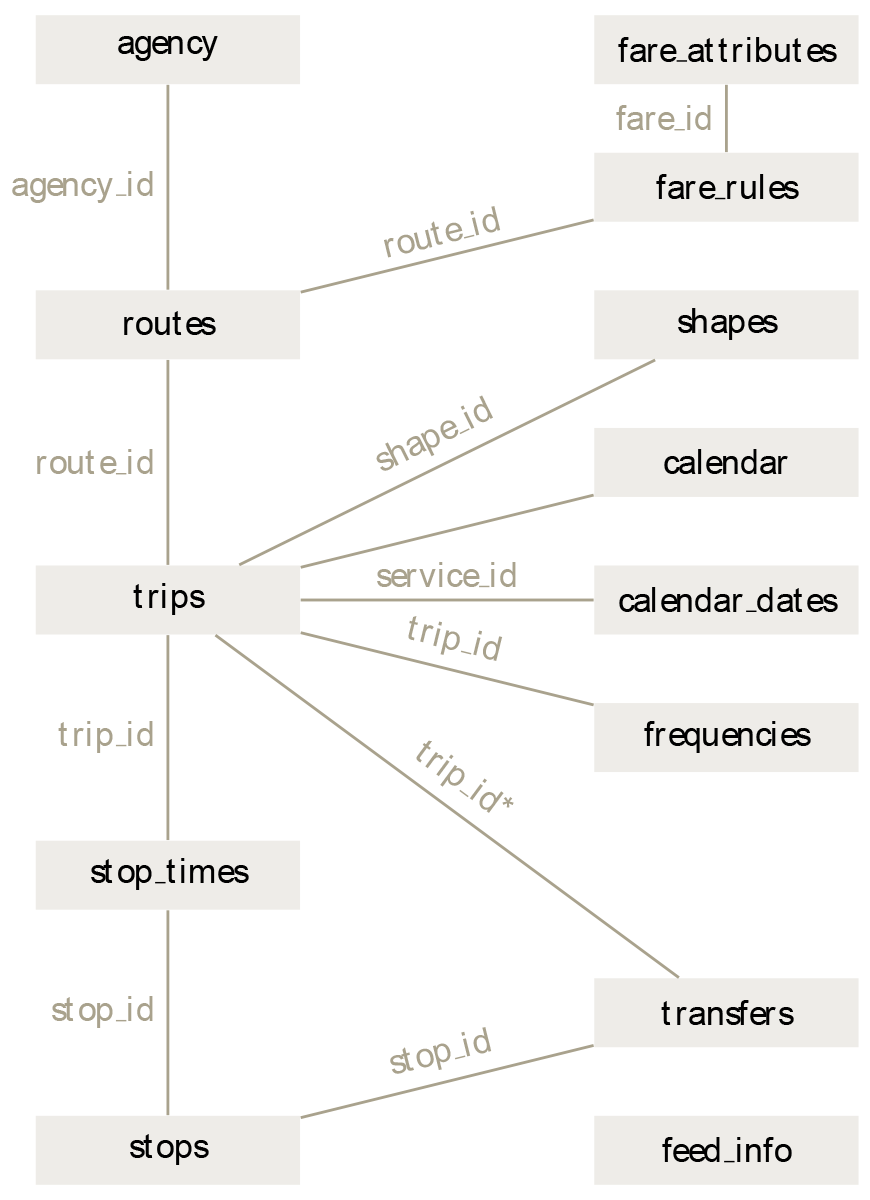
\includegraphics[width=0.5\textwidth]{GTFS_class_diagram.png}
		\caption[GTFS structuur]{De bestandsstructuur van GTFS data.}
	\label{fig:ldfAxis}
\end{figure}
% TODO: visueler maken wat GTFS juist is
 
Anderzijds zijn er traditionele Remote Procedure Call (RPC) zoals iRail\footnote{https://irail.be}, die beschikken over verschillende endpoints die specifieke vragen kunnen beantwoorden. Achterliggend kunnen zware berekeningen uitvoeren of grote databases raadplegen zonder dat de gebruiker hier nadeel van ondervindt. Deze antwoorden zijn rechtstreeks bruikbaar voor de client toepassing, maar bieden enkel een antwoord op één specifieke vraag. Een andere vraag, al dan niet door dezelfde client, vereist een nieuwe request naar de server, en zal een ander antwoord tot gevolg hebben. Elk verzoek naar de server vraagt relatief veel processortijd langs de serverkant. Een continue internetverbinding is dus vereist, en server-side is een potentieel grote en dure infrastructuur nodig om aan alle vragen te voldoen. Een ander belangrijk nadeel bij deze techniek is dat deze data moeilijk te combineren zijn met andere datasets. Een route plannen die gebruik maakt van meerdere openbaar vervoer aanbieders is enkel mogelijk als iemand een API aanbiedt die achterliggend door meerdere datasets zoekt. Simpelweg twee API's combineren is niet mogelijk.

\begin{figure}
	\centering
	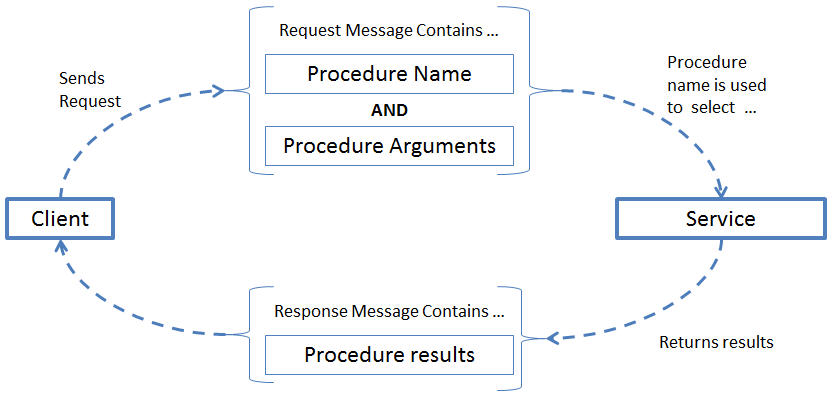
\includegraphics[width=0.80\textwidth]{RPC_API.jpg}
	\caption[RPC structuur]{De werkwijze van een RPC API.}
	\label{fig:ldfAxis}
\end{figure}

Deze twee methodes zijn elkaars tegengestelde. Ontwikkelaars moeten kiezen voor data die compact maar complex, en slechts indirect bruikbaar is, of voor een vraag-antwoord systeem wat voor elke nieuwe vraag een nieuw verzoek naar een server moet maken. Aan de IDLab onderzoeksgroep aan UGent is onderzoek gedaan naar Linked Connections (LC)\footnote{https://linkedconnections.org}, een nieuw formaat dat een nieuw evenwicht tracht te vinden. Alle vertrekken van alle voertuigen worden in één chronologische lijst verzameld, waarbij de lijst kan opgevraagd worden volgens vaste tijdsintervallen met een grootteorde van enkele minuten. Hierdoor hoeft de server enkel deze lijst in fragmenten aan te bieden, waarbij alle clients dezelfde informatie krijgen. De clients dienen zelf nog berekeningen te maken, maar deze zijn relatief eenvoudig vergeleken met de berekeningen die nodig zijn om een GTFS feed te verwerken. Data in het Linked Connections formaat kunnen eenvoudig toegankelijk gemaakt worden via een open-source serverapplicatie\footnote{https://github.com/julianrojas87/linked-connections-server/}.

\begin{figure}
	\centering
		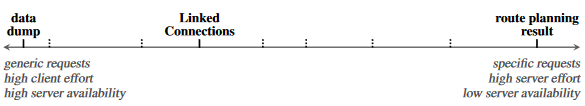
\includegraphics[width=0.80\textwidth]{ldfAxis.png}
	\caption[Routeplanning HTTP interfaces op de LDF as]{De Linked Data Fragments as illustreert dat alle HTTP interfaces data fragmenten aanbieden, maar verschillen in hoe specifiek de aangeboden data is, en dus de moeilijkheid om deze aan te maken~\citep{verborgh14}. In deze figuur is de as toegepast op HTTP interfaces voor routeplanning~\citep{colpaert15}.}
	\label{fig:ldfAxis}
\end{figure}

\section{Wat is user-perceived performance?}
\label{sec:what_is_user_perceived_performance}
Elke interface voor het ophalen van data heeft specifieke eigenschappen zoals latency, performance, cache hergebruik,~...~\citep{verborgh16}. Wanneer we verschillende technieken vergelijken door dezelfde user-agent, kunnen we de impact van de verschillende achterliggende technieken op de eindgebruiker onderzoeken. Hiervoor definiëren we de user-perceived performance. De user-perceived performance is de performance zoals de gebruiker deze ervaart, welke niet strikt gelijk hoeft te zijn aan de performance van technische component. De user-perceived latency werd gedefinieerd in 2000 door Roy T. Fielding gedefinieerd als de tijd tussen het selecteren van een link en het renderen van een bruikbaar resultaat~\citep{fielding99}. Latency treedt op op verschillende punten: 
\begin{enumerate}
	\item de tijd die de client nodig heeft om actie te ondernemen 
	\item de tijd die nodig is voor voorbereidende acties
	\item de tijd om een verzoek te verzenden
	\item de tijd die de server nodig heeft om te antwoorden
	\item de tijd die nodig is om het antwoord te verzenden
	\item de tijd voor het antwoord te verwerken en weer te geven
\end{enumerate}
Terwijl enkel stappen 3, 4 en 5 rechtstreeks afhankelijk zijn van het netwerk, kunnen al deze stappen beïnvloed worden door de gebruikte techniek \citep{fielding99}.

Ondertussen zijn we geëvolueerd naar een wereld waarin data vaak mobiel geconsumeerd worden: 78\% van de Vlamingen beschikt over een smartphone, 80,5\% beschikt over een laptop. Slechts 41,8\% beschikt over een desktop-computer~\citep{digimeter17}. Hierbij zijn er ook andere aspecten die meespelen in de user experience: batterijgebruik en offline toegang tot data vormen een aanzienlijke factor in de user experience. Een applicatie presteert beter wanneer deze dezelfde data kan weergeven met aanzienlijk minder energieverbruik, of wanneer deze consistent goed presteert, ook wanneer netwerk slecht of niet beschikbaar is. Hoewel de user-perceived performance nog steeds gedomineerd wordt door de tijd tussen het selecteren van een link en het renderen van een bruikbaar resultaat, dienen we dus ook deze andere aspecten in rekening te brengen. Mobiele gebruikers hebben ook nog steeds angst om te veel data te verbruiken~\citep{ammelrooy17}.

% TODO: zal dit zo blijven of is er een trend ivm angst over datalimiet?

\section{Probleemstelling en doel van de masterproef}
\label{sec:problem}

Linked Connections werd ontwikkeld met de bedoeling een evenwicht te vinden tussen data dumps en RPC API's. In plaats van elke query op een server te beantwoorden, wordt een gelinkte lijst van connecties gepubliceerd. Linked Connections laat hierdoor toe om queries te beantwoorden door middel van een lineair groeiende lijst van connecties~\citep{colpaert15}. Bovendien gebruiken alle user-agents dezelfde lijst, waardoor deze zeer cachebaar is. Bij stijgende belasting daalt de tijd die nodig is per verzoek \citep{colpaert17}.

Terwijl de cost-efficiency van Linked Connections reeds is aangetoond, waarbij Linked Connections hetzelfde aantal verzoeken kan beantwoorden met slechts 25\% van de rekencapacteit\citep{colpaert17,Melendez17}, is er nog geen onderzoek gebeurt naar de user-perceived performance van een user-agent wanneer deze gebruik maakt van Linked Connections, vergeleken met wanneer deze zelfde user-agent gebruik maakt van een traditionele RPC API. 

In deze studie richten we ons specifiek op routeplanning gebruik makend van mobiele toestellen. Deze toestellen hebben minder processorkracht en geheugen vergeleken met traditionele computers, maar ook bandbreedte en beschikbaarheid van internet zijn vaak beperkt. In het slechtste geval is er geen netwerkverbinding, waarbij enkel een cache beschikbaar is. Verder zullen we ons specifiek richten op het verschil tussen een RPC REST API gebaseerd op Linked Connections~\citep{colpaert17} en de originele Linked Connections webserver. Als user-agent zullen we een fork van de Android HyperRail\footnote{https://hyperrail.be} applicatie gebruiken, gemodificeerd om de genoemde API's te gebruiken. Door deze testopstelling zijn de oorspronkelijke data, de server hardware, de user-agent en de client hardware gelijk bij elke vergelijking. Enkel het formaat voor serverinteracties en transport van data zal verschillen.

Om routes te berekenen zullen we gebruik maken van het Connection Scan Algorithm (CSA)~\citep{strasser13,strasser14,strasser17}. Dit algoritme vereist een op vertrektijd gesorteerde lijst van vertrekken. Dit is de exacte definitie van de LinkedConnections knowledge graph, waardoor dit algoritme zonder al te veel modificaties toegepast kan worden. Fragmenten kunnen hierbij geladen worden op het moment dat ze nodig zijn. We zullen dezelfde implementatie gebruiken zowel bij de client-side API als bij de server-side API om zo correct mogelijke resultaten te behalen. 

In eerste instantie zal een traditionele (RPC) API geschreven worden welke gebruik maakt van de Linked Connections fragmenten op de Solid State Disk (SSD) van de server. Deze API zal endpoints bevatten voor het tonen van vertrekken en aankomsten per station, het berekenen van routes, en voor het weergeven van het traject per trein. 
Vervolgens zal een API zonder specifieke server-side geïmplementeerd worden in de applicatie. Deze zal dezelfde informatie ter beschikking stellen in de applicatie, maar zal hiervoor enkel (delen van) de gelinkte lijst met vertrekken downloaden. 

Eenmaal beide API's volledig geïmplementeerd zijn, zal de user-experienced performance onderzocht worden. Hiertoe worden begeleide user tests gehouden, waarbij een aantal testgebruikers afwisselend met beide API's hun dagelijkse opzoekingen zullen uitvoeren, waarna ze aan de hand van een vragenlijst bevraagd zullen worden naar hun ervaringen en voorkeuren. Het is essentieel om de subjectieve ervaringen van gebruikers te bevragen, gezien verschillende gebruikers mogelijk verschillende afwegingen maken. We verwachten dat sommige gebruikers offline toegang waardevol zullen vinden, terwijl anderen mogelijk geen belang hechten aan offline toegang. Ook zal er technische data verzameld worden, zoals geheugen- en processorgebruik, laadtijden, en batterijverbruik. 

Deze masterproef zal gebruik maken van data afkomstig van de NMBS om routeplanning en realtime data over treinen in België weer te geven. Door de bron van de data te vervangen kan dit onderzoek ook toegepast worden op andere openbaar vervoer maatschappijen die gebruik maken van tijdsschema's, ongeacht het soort voertuig dat gebruikt wordt.

\section{Onderzoeksvraag}
 
 \paragraph{Hypothese 1} De gebruiker ervaart de mogelijkheid voor offline zoekopdrachten als een meerwaarde.
 
 \paragraph{Hypothese 2} De gebruiker ervaart de mogelijkheid om voorkeuren voor routes in te stellen (overstaptijd, toegankelijkheid, ...) als een meerwaarde.
 
 \paragraph{Onderzoeksvraag} Verbetert de user experience en user perceived perforance van een applicatie voor openbaar vervoer wanneer gebruik gemaakt wordt van Linked Connections in plaats van traditionele RPC API's?
\begin{savequote}[0.55\linewidth]
	``Inspirational quote''
	\qauthor{\textasciitilde Source}
\end{savequote}

\chapter{Implementatie}
Om een zo eerlijk mogelijke vergelijking te bekomen, zullen we zowel bij de client-side API als de server-side API dezelfde algorithmes toepassen. Gezien de jonge leeftijd van het Linked Connections framework zijn er nog geen algoritmes beschikbaar om deze data te verwerken. We zullen de ontwikkeling van deze algoritmen bespreken, met speciale aandacht voor het routeplanning algoritme vanwege de hogere complexiteit en de uitgebreide mogelijkheden.

\section{Linked Connections formaat}

In plaats van een dump van planningsdata of een volledige routeplanner te publiceren, publiceert Linked Connections paren van vertrek en aankomst voor elke treinrit, telkens van een station tot het volgende. Deze paren worden gesorteerd volgens vertrektijd. Hierna wordt deze lijst van paren gesplitst, om pagina's van gelijke grootte of gelijke tijdsduur te bekomen. Deze fragmenten kunnen gepubliceerd worden via HTTP als \foreign{JSON-LD}\footnote{https://json-ld.org/}, waarbij user-agents kunnen kiezen welke pagina's ze opvragen. Links in de gepubliceerde documenten zorgen ervoor dat user-agents steeds weten welke pagina ze als volgende moeten laden \citep{linkedconnections18}.

Om bovenstaande methode in de praktijk om te zetten, wordt gebruik gemaakt van de open source LC-Server\footnote{https://github.com/julianrojas87/linked-connections-server/}. Om GTFS om te zetten naar Linked Connections, wordt er achterliggend gebruik gemaakt van de gtfs2lc tool\footnote{https://github.com/linkedconnections/gtfs2lc}.

Deze data zijn publiek toegankelijk via https://graph.irail.be/.

\subsection{Vraag- en antwoordformaat}
Om een pagina met data op te halen, wordt een verzoek gemaakt naar de API, waarbij de vervoersmaatschappij en het gewenste tijdstip in ISO8601 formaat in de URL opgenomen worden.  Codefragment \ref{code:linkedconnections-response} toont een ingekort resultaat voor de vertrekken bij de NMBS op 20 maart 2018, 12:30. De volledige specificatie kan teruggevonden worden op de LC website\footnote{https://linkedconnections.org/specification/1-0}.

Verzoek: \inlinecode{https://graph.irail.be/sncb/connections?departureTime=2018-03-20T12:30:00.000Z}

Een voorbeeld van een LC pagina zien we in fragment \ref{code:2:linkedconnections-response}, met volgende data:
\begin{enumerate}
	\item \foreign{@context}: Deze lijst definieert de gebruikte namespaces en velden
	\item \foreign{hydra:next} en  \foreign{hydra:previous}: Links naar de pagina met respectievelijk de volgende en de voorgaande data
	\item \foreign{hydra:search}: Informatie over de huidige pagina
	\item \foreign{@graph}: Deze lijst bevat de eigenlijke data. Elk vertrek bevat de volgende informatie:
	\begin{enumerate}
			\item \foreign{departureStop}: De URI welke het station van vertrek uniek identificeert.
			\item \foreign{arrivalStop}: De URI welke het station van aankomst uniek identificeert.	\item departureTime, arrivalTime: De geplande tijden, respectievelijk bij vertrek en aankomst.
			\item \foreign{departureDelay}, \foreign{arrivalDelay}: De vertraging, respectievelijk bij vertrek en aakomst.
			\item \foreign{direction}: De richting van dit voertuig, wat vaak ook op de lichtkrant van het voertuig weergegeven wordt.
			\item \foreign{gtfs:trip}: Een URI welk de rit van het voertuig uniek identificeert
			\item \foreign{gtfs:route}: Een URI welk de route van het voertuig uniek identificeert
			\item \foreign{gtfs:pickupType} en \foreign{gtfs:dropOffType}: geeft aan of reizigers al dan niet kunnen op- of afstappen bij respectievelijk vertrek en aankomst
	\end{enumerate}
\end{enumerate}

\begin{code}
	\begin{minted}[breaklines,tabsize=2]{json}
		
		{
			"@context": {
			 "xsd": "http://www.w3.org/2001/XMLSchema#",
			"lc": "http://semweb.mmlab.be/ns/linkedconnections#",
			"hydra": "http://www.w3.org/ns/hydra/core#",
			"gtfs": "http://vocab.gtfs.org/terms#",
			"Connection": "lc:Connection",
			"...": "..."
			},
			"@id": "https://graph.irail.be/sncb/connections?departureTime=2018-03-20T12:30:00.000Z",
			"@type": "hydra:PagedCollection",
			"hydra:next": "https://graph.irail.be/sncb/connections?departureTime=2018-03-20T12:40:00.000Z",
			"hydra:previous": "https://graph.irail.be/sncb/connections?departureTime=2018-03-20T12:20:00.000Z",
			"hydra:search": {
				"..."
			},
			"@graph": [
				{
				"@id": "http://irail.be/connections/8822228/20180320/S11961",
				"@type": "Connection",
				"departureStop": "http://irail.be/stations/NMBS/008822228",
				"arrivalStop": "http://irail.be/stations/NMBS/008822210",
				"departureTime": "2018-03-20T12:30:00.000Z",
				"departureDelay": 60,
				"arrivalTime": "2018-03-20T12:32:00.000Z",
				"arrivalDelay": 0,
				"direction": "Anvers-Central",
				"gtfs:trip": "http://irail.be/vehicle/S11961/20180320",
				"gtfs:route": "http://irail.be/vehicle/S11961",
				"gtfs:pickupType": "gtfs:Regular",
				"gtfs:dropOffType": "gtfs:Regular"
				},
				{"...":"..."}
			]
		}
	\end{minted}
\caption{Voorbeeld Linked Connections Formaat}
\label{code:2:linkedconnections-response}
\end{code}
\section{Connection Scan Algoritme}
Routeplanning wordt vaak opgelost met behulp van (een variant op) het algoritme van Dijkstra ~\citep{strasser13}. Toepassingen die gebruik maken van Dijkstra vereisen echter een graaf en een \foreign{priority queue}. Naast de impact op prestaties die deze eisen vormen, beperkt een graaf ook de flexibiliteit. De \foreign{open world assumption} stelt dat er steeds andere stopplaatsen wiens bestaan we (nog) niet kennen. Het opstellen van een graaf zou vereisen dat we alle gegevens eerst volledig moeten downloaden, terwijl Linked Connections net goed geschikt is voor streaming.


Het Connection Scan Algoritme (CSA) werd voor het eerst beschreven door Ben Strasser in 2013~\citep{strasser13}. Dit algoritme vereist van een lijst met vertrekken gesorteerd op vertrektijd. Hiermee worden alle routes in een tijdsinterval efficiënt berekend\citep{strasser14,strasser17}. In tegenstelling tot Dijkstra's algoritme is er geen graaf of \foreign{priority queue} benodigd. Waar andere algoritmen ofwel enkel op kleine netwerken performant zijn, ofwel niet altijd de  best mogelijke route vinden, kan CSA de optimale route in grote netwerken toch efficiënt vinden~\citep{strasser14}. In de praktijk is het vooral belangrijk om snel rekening te kunnen houden met vertragingen bij vertrek of aankomst\citep{strasser14,strasser17}. CSA berekent oorspronkelijk de snelste route, al is dit duidelijk niet altijd de route die de gebruiker wenst. Zo kan de snelste route nog steeds een station meermaals bezoeken, of kan men van een trein afstappen om later op deze zelfde trein weer op te stappen. Een oplossing hiervoor is om het aantal overstappen te beperken\citep{strasser14}.

Naast de tijd van aankomst, zijn er nog een aantal andere criteria die vaak geoptimaliseerd worden. Het populairste tweede criterium is het aantal overstappen, gevolgd door de prijs \citep{strasser17}. Optimalisatie van de prijs is echter zeer complex vanwege de complexe tariefplannen bij openbaar vervoer\citep{muller06}. Dit valt buiten de context van deze masterproef.

\subsection{Implementatie en aanpassingen}
De werking en implementatie van CSA worden behandeld in~\citep{strasser17}. Dit algoritme kan zonder veel wijzigingen geïmplementeerd worden in zowel Java\footnote{https://github.com/Bertware/linkedconnections-android-client/blob/master/Hyperrail/src/main/java/be/hyperrail/android/irail/implementation/linkedconnections/RouteResponseListener.java} als PHP\footnote{https://github.com/hyperrail/lc2irail/blob/master/app/Http/Repositories/ConnectionsRepository.php}.

Wanneer dit algoritme geïmplementeerd wordt merken we echter duidelijke verschillen met de voorgestelde routes door de NMBS. Deze verschillen manifesteren zich vooral in de keuze van het station waar er overgestapt moet worden tussen twee treinen, en de keuze van de tussenliggende treinen indien er meer dan één overstap is. Zo is het mogelijk dat er wordt aangeraden om een trein te nemen langs Brussel Zuid en Centraal tot Noord, om van daar een andere trein te nemen die op zijn beurt van Brussel-Noord langs Centraal naar Zuid rijdt.
Verder zullen we ook nog aanpassingen doorvoeren om eenvoudig het aantal overstappen te beperken, en om op een betere manier aan \foreign{journey-extraction} te doen.

De implementatie en evolutie van het CSA algoritme worden uitgelegd aan de hand van code fragmenten in Java. Er wordt verondersteld dat sectie 4.2 van \cite{strasser17} gekend is. De code is asynchroon, waarbij na het laden van de eerste Linked Connections pagina een callback functie opgeroepen wordt om deze pagina te verwerken. Afhankelijk van het resultaat van deze verwerking, wordt er een nieuwe pagina opgevraagd, of wordt het resultaat doorgegeven aan de oproepende code door middel van callbacks.

Allereerst dienen we twee wijzigingen door te voeren aan de gegevensstructuren. De arrays S en T zijn vervangen door een Map, waardoor we onbeperkt nieuwe stations en trips kunnen toevoegen, en deze kunnen opvragen op basis van hun URI. Dit maakt het algoritme geschikt om te werken rekening houdend met de open world assumption. In de datastructuur voor een voertuig (fragment \ref{code:2:trips}) houden we niet enkel bij wanneer we zouden aankomen, maar ook met hoeveel overstappen (beginnend na het opstappen op deze trein) we zouden aankomen, en waar we moeten afstappen van deze trein. Dit laatste is essentieel om niet enkel de aankomsttijd, maar ook de exacte route met alle overstappen te kunnen weergeven. 

\begin{code}
	\begin{minted}[breaklines,tabsize=2]{java}
	class TrainTriple {
		/**
		* The arrival time at the final destination
		*/
		DateTime arrivalTime;
		
		/**
		* The number of transfers until the destination when hopping on to this train
		*/
		int transfers;
		
		/**
		* The arrival connection for the next transfer or arrival
		*/
		LinkedConnection arrivalConnection;
	}
	
	\end{minted}
	\caption[CSA: Gegevensstructuur voor trips]{In tegenstelling tot~\cite{strasser17} wordt niet enkel de aankomsttijd, maar ook de afstaphalte en het aantal overstappen bijgehouden per trip.}
	\label{code:2:trips}
\end{code}

Ook de paren van vertrek en aankomsttijd per station, zogenoemde profielen, worden vervangen door een meer uitgebreide gegevensstructuur, zichtbaar in fragment \ref{code:2:stations}. Naast de vertrek en aankomsttijd houden we nu ook de connectie bij waarmee we vertrekken in dit station op dit tijdstip, en de connectie waarmee we aankomen in het volgend station waar we moeten over- of afstappen. Ook het aantal overstappen, beginnend met tellen na het opstappen in dit station, wordt bijgehouden.

\begin{code}
\begin{minted}[breaklines,tabsize=2]{java}
  class StationQuadruple {
	/**
	* The departure time in this stop
	*/
	DateTime departureTime;
	
	/**
	* The arrival time at the final destination
	*/
	DateTime arrivalTime;
	
	/**
	* The departure connection in this stop
	*/
	LinkedConnection departureConnection;
	
	/**
	* The arrival connection for the next transfer or arrival
	*/
	LinkedConnection arrivalConnection;
	
	/**
	* The number of transfers between standing in this station and the destination
	*/
	int transfers;
}
	\end{minted}
		\caption[CSA: Gegevensstructuur voor stopprofielen]{In tegenstelling tot~\cite{strasser17} wordt niet enkel de vertrek- en aankomsttijd, maar ook het aantal overstappen en de afstaphalte van de volgende trein bijgehouden.}
	\label{code:2:stations}
\end{code}

Wanneer we de ingeladen connecties willen verwerken, filteren we alle connecties uit de pagina die ofwel te vroeg, ofwel te laat vallen. Zoals te zien in fragment \ref{code:2:csaloop} stellen we een flag in wanneer we voorbij de vroegste vertrekdatum zijn. In dit geval zullen we na het overlopen van deze lijst geen nieuwe lijsten meer ophalen. Door deze methode toe te passen kunnen we nieuwe pagina's inladen wanneer deze nodig zijn, zonder te veel op voorhand in te moeten laden.

\begin{code}
\begin{minted}[breaklines,tabsize=2]{java}
	if (data.connections.length == 0) {
		mLinkedConnectionsProvider.getLinkedConnectionByUrl(data.previous, this, this, null);
		return;
	}
	
	boolean hasPassedDepartureLimit = false;
	for (int i = data.connections.length - 1; i >= 0; i--) {
		LinkedConnection connection = data.connections[i];
		
		if (connection.departureTime.isAfter(mArrivalLimit)) {
			continue;
		}
		if (connection.departureTime.isBefore(mDepartureLimit)) {
			hasPassedDepartureLimit = true;
			continue;
		}
		
		...
	}
	\end{minted}
			\caption[CSA: Overlopen van connecties]{Connecties worden overlopen volgens dalende vertrektijd. Er worden beperkingen gesteld op vertrek- en aankomsttijd.}
	\label{code:2:csaloop}
\end{code}

Het bepalen van T1 en T2 spreekt voor zich, en loopt vrijwel gelijk aan de implementatie uit \cite{strasser17}. In fragment \ref{code:2:csaT1T2} zien we hoe het aantal overstappen wordt bepaald. In het geval dat er geen aankomst mogelijk is (binnen de beperkte tijd) stellen we zowel de aankomsttijd als het aantal overstappen in op een onrealistisch hoog getal. Dit vereenvoudigt de code latere aanzienlijk, aangezien er geen rekening gehouden hoeft te worden met het mogelijk leeg zijn van variabelen.
\begin{code}
	\begin{minted}[breaklines,tabsize=2]{java}
	 	if (Objects.equals(connection.arrivalStationUri, mRoutesRequest.getDestination().getSemanticId())) {
			T1_walkingArrivalTime = connection.arrivalTime;
			T1_transfers = 0;
		} else {
			T1_walkingArrivalTime = infinite;
			T1_transfers = 999;
		}

		// Determine T2, the first possible time of arrival when remaining seated
		if (T.containsKey(connection.trip)) {
			T2_stayOnTripArrivalTime = T.get(connection.trip).arrivalTime;
			T2_transfers = T.get(connection.trip).transfers;
		} else {
			T2_stayOnTripArrivalTime = infinite;
			T2_transfers = 999;
		}	
		\end{minted}
					\caption[CSA: Bepalen van aankomsttijden]{Het aantal overstappen wordt bepaald bij het bepalen van minimale aankomsttijden}
		\label{code:2:csaT1T2}
\end{code}

Bij de bepaling van T3, terug te vinden in fragment \ref{code:2:csaT3}, maken we de eerste grote afwijking van het oorspronkelijk algoritme. Om te bepalen of een overstap mogelijk is, moeten er reeds profielen voor dit station bekend zijn. Indien dit het geval is, gaan we op zoek naar het profiel waarbij er genoeg tijd is om over te stappen, maar waarbij het aantal overstappen het maximum aantal niet overschrijdt. 
Wanneer we een overstap vinden die aan deze voorwaarden voldoet, verhogen we het aantal overstappen ook met één. Deze aanpak is eenvoudiger dan de array-gebaseerde aanpak omschreven in \cite{strasser17}. Het voordeel van deze aanpak is dat automatisch alle snelste opties worden bijgehouden, zolang hun aantal overstappen onder het maximum blijft. 

In plaats van de door \cite{strasser17} voorgestelde verhoging van de aankomsttijd met één, om zo routes met een gelijke aankomsttijd maar minder overstappen voorkeur te geven, verhogen we hier de aankomsttijd met een vooraf gedefinieerd aantal seconden. Dit aantal geeft aan hoeveel seconden we langer op een trein wensen te zitten, in plaats van over te stappen. Door dit in te stellen op 240, wordt aangegeven dat een route die er tot 4 minuten langer over doet, met een overstap minder, toch de voorkeur krijgt over de snellere route met meer overstappen. Dit is een eerste veld dat door gebruikers ingesteld kan worden om de routes te personaliseren.

\begin{code}
	\begin{minted}[breaklines,tabsize=2]{java}
		// Determine T3, the time of arrival when taking the best possible transfer in this station
		if (S.containsKey(connection.arrivalStationUri)) {
			int position = S.get(connection.arrivalStationUri).size() - 1;
			StationQuadruple quadruple = S.get(connection.arrivalStationUri).get(position);
		
			while (
				(quadruple.departureTime.minusSeconds(transferSeconds).getMillis() <= connection.arrivalTime.getMillis() ||
				quadruple.transfers >= maxTransfers) &&  
				position > 0
			) {
				position--;
				quadruple = S.get(connection.arrivalStationUri).get(position);
			}
			if (quadruple.departureTime.minusSeconds(transferSeconds)
					.isAfter(connection.arrivalTime) && 
					quadruple.transfers <= maxTransfers) {
				T3_transferArrivalTime = quadruple.arrivalTime.plusSeconds(extraTimeInsteadOfTransfer);
				// Using this transfer will increase the number of transfers with 1
				T3_transfers = quadruple.transfers + 1;
			} else {
				// When there isn't a reachable connection, transferring isn't an option
				T3_transferArrivalTime = infinite;
				T3_transfers = 999;
			}
		} else {
			// When there isn't a reachable connection, transferring isn't an option
			T3_transferArrivalTime = infinite;
			T3_transfers = 999;
		}
		\end{minted}
						\caption[CSA: Bepalen van aankomsttijden]{Bij een eventuele overstap worden ook extra factoren in rekeningen gebracht.}
		\label{code:2:csaT3}
\end{code}
Bij het bepalen van de vroegste aankomsttijd (fragment \ref{code:2:csaT3}), wordt nu ook het aantal overstappen dat bij deze aankomsttijd hoort bepaald, en de connectie waar van de trein afgestapt wordt. We geven bij gelijke aankomsttijden de voorkeur aan overstappen: aangezien de vertrekkende voertuigen volgens dalende vertrektijd overlopen worden, geven we dus de voorkeur aan zo vroeg mogelijk overstappen. Dit geeft extra marge binnen de trip.
\begin{code}
\begin{minted}[breaklines,tabsize=2]{java}
DateTime Tmin;
LinkedConnection exitTrainConnection;
int numberOfTransfers;

if (T3_transferArrivalTime.getMillis() <= T2_stayOnTripArrivalTime.getMillis()) {
	Tmin = T3_transferArrivalTime;
	exitTrainConnection = connection;
	numberOfTransfers = T3_transfers;
} else {
	Tmin = T2_stayOnTripArrivalTime;
	if (T2_stayOnTripArrivalTime.isBefore(infinite)) {
		exitTrainConnection = T.get(connection.trip).arrivalConnection;
	} else {
		exitTrainConnection = null;
	}
	numberOfTransfers = T2_transfers;
}
// For equal times, we prefer just arriving.
if (T1_walkingArrivalTime.getMillis() <= Tmin.getMillis()) {
	Tmin = T1_walkingArrivalTime;
	exitTrainConnection = connection;
	numberOfTransfers = T1_transfers;
}

if (Tmin.isEqual(infinite)) {
	continue;
}
		\end{minted}
		\caption[CSA: Bepalen van vroegste aankomsttijd]{Bepalen van de vroegste aankomsttijd}
		\label{code:2:csaMin}
\end{code}
Door de extra toevoegingen voor journey extraction en het optimaliseren van de routes, is het bijwerken van de gegevenstructuren aanzienlijk ingewikkelder vergeleken met de originele implementatie. Voor voertuigen houden we niet langer enkel de aankomsttijd, maar ook de afstap halte bij. Hierbij verkiezen we de halte waarlangs we zo snel mogelijk aankomen, maar bij gelijke aankomsttijd wensen we een zo lang mogelijke periode voor de overstap. Wanneer de aankomsttijd gelijk is, onderzoeken we of de nieuwe afstap halte (de connectie die op dit moment onderzocht wordt) meer tijd voor een overstap geeft. Indien dit het geval is, werken we de afstap halte bij. Het bijwerken van een bestaande trip is zichtbaar in fragment \ref{code:2:csaT}.
\begin{code}
	\begin{minted}[breaklines,tabsize=2]{java}
	
		if (Tmin.isEqual(T.get(connection.trip).arrivalTime) && 
			T3_transferArrivalTime.isEqual(T2_stayOnTripArrivalTime) &&
			S.containsKey(T.get(connection.trip).arrivalConnection.arrivalStationUri) &&
			S.containsKey(connection.arrivalStationUri)
		) {
			LinkedConnection currentTrainExit = T.get(connection.trip).arrivalConnection;
			
			StationQuadruple quad = new StationQuadruple();
			quad.departureTime = connection.departureTime;
			quad.departureConnection = connection;
			quad.arrivalTime = Tmin;
			
			// Current situation
			quad.arrivalConnection = currentTrainExit;
			Duration currentTransfer = new Duration(currentTrainExit.arrivalTime, getFirstReachableConnection(quad).departureTime);
			// New situation
			quad.arrivalConnection = exitTrainConnection;
			Duration newTransfer = new Duration(exitTrainConnection.arrivalTime, getFirstReachableConnection(quad).departureTime);
	
			if (newTransfer.isLongerThan(currentTransfer)) {
				TrainTriple triple = new TrainTriple();
				triple.arrivalTime = Tmin;
				triple.arrivalConnection = exitTrainConnection;
				triple.transfers = numberOfTransfers;
				T.put(connection.trip, triple);
			}
		}
		
		if (Tmin.isBefore(T.get(connection.trip).arrivalTime)) {
			TrainTriple triple = new TrainTriple();
			triple.arrivalTime = Tmin;
			triple.arrivalConnection = exitTrainConnection;
			triple.transfers = numberOfTransfers;
			T.put(connection.trip, triple);
		}
	\end{minted}
	\caption[CSA: Bijwerken T]{Bijwerken van de trips gegevensstructuur.}
	\label{code:2:csaT}
\end{code}

Het bijwerken van de stopprofielen, zichtbaar in fragment \ref{code:2:csaS}, is lichtjes aangepast om de efficiëntie te verhogen. De vroegste vertrekken worden nu achteraan toegevoegd. Door deze aanpassing, en het gegeven dat de vertrektijd van de huidige connectie gelijk of kleiner dan de vertrektijd van alle vorige connecties is, hoeven we nu enkel het laatste profiel in de lijst te evalueren. Als de vertrektijd kleiner of gelijk is, moet de aankomsttijd kleiner zijn. we controleren dus enkel of de aankomsttijd kleiner is, en zo ja, of de vertrektijd kleiner of gelijk is. Afhankelijk van deze laatste controle voegen we een nieuw item toe aan de lijst, of vervangen we het laatste. Aangezien we telkens enkel toevoegen wanneer de aankomsttijd vroeger ligt, zal deze lijst altijd gesorteerd zijn volgens dalende aankomsttijd. Hiermee is bewezen dat deze optimalisatie correct is, en een beter alternatief voor het overlopen van de volledige lijst.

\begin{code}
	\begin{minted}[breaklines,tabsize=2]{java}
		StationQuadruple quad = new StationQuadruple();
		quad.departureTime = connection.departureTime;
		quad.arrivalTime = Tmin;
		
		// Additional data for journey extraction
		quad.departureConnection = connection;
		quad.arrivalConnection = T.get(connection.trip).arrivalConnection;
		quad.transfers = numberOfTransfers;
		
		if (S.containsKey(connection.departureStationUri)) {
			int numberOfPairs = S.get(connection.departureStationUri).size();
			StationQuadruple existingQuad = S.get(connection.departureStationUri).get(numberOfPairs - 1);
			if (quad.arrivalTime.isBefore(existingQuad.arrivalTime)) {
				if (quad.departureTime.isEqual(existingQuad.departureTime)) {
					S.get(connection.departureStationUri).remove(numberOfPairs - 1);
					S.get(connection.departureStationUri).add(numberOfPairs - 1, quad);
				} else {
					S.get(connection.departureStationUri).add(quad);
				}
			}
		} else {
			S.put(connection.departureStationUri, new ArrayList<StationQuadruple>());
			S.get(connection.departureStationUri).add(quad);
		}
	\end{minted}
	\caption[CSA: Bijwerken S]{Bijwerken van de stops gegevensstructuur.}
	\label{code:2:csaS}
\end{code}
De lijst met volledige routes reconstrueren (fragment \ref{code:2:csaJourneyExtraction}) is relatief eenvoudig. Voor elk profiel horend bij de stoplocatie van waar de reiziger vertrekt, volgen we de vertrek- en aankomstconnecties. Om bij elke tussenstop de juiste connectie te vinden waarmee de reis verder zal gezet worden, vergelijken we de aankomsttijd uit het stopprofiel waaruit we vertrokken, met de aankomsttijden uit de stopprofielen van de tussenstop (fragment \ref{code:2:csaJourneyExtractionReachable}). Wanneer deze gelijk zijn, hebben we het volgende deel van de reis gevonden.
\begin{code}
	\begin{minted}[breaklines,tabsize=2]{java}
		// Results? Return data
		Route[] routes = new Route[S.get(mRoutesRequest.getOrigin().getSemanticId()).size()];
		
		int i = 0;
		for (StationQuadruple quad : S.get(mRoutesRequest.getOrigin().getSemanticId())
		) {
			// it will iterate over all legs
			StationQuadruple it = quad;
			List<RouteLeg> legs = new ArrayList<>();
			
			while (!Objects.equals(it.arrivalConnection.arrivalStationUri, mRoutesRequest.getDestination().getSemanticId())) {
				// use it.departureConnection and it.arrivalConnection to construct legs of this journey
				legs.add(...);
				it = getFirstReachableConnection(it);
			}
			
			routes[i++] = new Route(legs);
		}
	\end{minted}
	\caption[CSA: Journey extraction]{Journey Extraction door middel van post-processing}
	\label{code:2:csaJourneyExtraction}
\end{code}
\begin{code}
	\begin{minted}[breaklines,tabsize=2]{java}
		private StationQuadruple getFirstReachableConnection(StationQuadruple arrivalQuad) {
			List<StationQuadruple> it_options = S.get(arrivalQuad.arrivalConnection.arrivalStationUri);
			int i = it_options.size() - 1;
				while (i >= 0 && it_options.get(i).arrivalTime.getMillis() != arrivalQuad.arrivalTime.getMillis() - 240 * 1000) {
				i--;
			}
			return it_options.get(i);
		}
	\end{minted}
	\caption[CSA: Journey extraction bij tussenstops]{Vinden van volgende vertrek bij tussenstop}
	\label{code:2:csaJourneyExtractionReachable}
\end{code}

\section{Vertrekken en aankomsten per station}

\section{Route van een trein}
% !TeX spellcheck = nl_NL
\begin{savequote}[0.55\linewidth]
	``Alice: How long is forever? White Rabbit: Sometimes, just one second. —  Alice's Adventures in Wonderland''
	\qauthor{\textasciitilde Lewis Carroll}
\end{savequote}

\chapter{Evaluatie}

\label{chap:onderzoek}
De user-perceived performantie kan afwijken van de werkelijke performantie. Dit verschil wordt voornamelijk bepaald door de interface van de applicatie. Zo ervaren gebruikers wachttijden als minder lang wanneer ze een gevoel van vooruitgang krijgen, door het gebruik van voortgangsbalken of andere visuele hints. Aangezien we bij dit onderzoek dezelfde applicatie voor beide API's gebruiken, zullen deze visuele hints de vergelijking van de user-perceived performance tussen de twee diensten niet beïnvloeden. Echter biedt Linked Connections de mogelijkheid tot incrementele resultaten: nog tijdens het laden kunnen al snel eerste resultaten weergegeven worden, waardoor de gebruiker deze techniek als sneller kan ervaren, ook al duurt het langer om een gelijk aantal resultaten op te halen. Ook voor LC2Irail zal de applicatie van incrementele resultaten gebruikmaken, echter is het hier steeds de server die bepaalt wanneer data verzonden worden. De server zal steeds pogen om een bepaald tijdsinterval te verwerken, of een bepaald aantal resultaten te  alvorens de client te antwoorden. Hierdoor kunnen de resultaten wel per tijdsinterval getoond worden, maar niet zo individueel als wanneer Linked Connections gebruikt wordt.

In figuur~\ref{fig:expectedserviceperceivedservice} zien we de factoren die bijdragen tot de verwachting van de gebruiker en de ervaring van de gebruiker. De user-experience wordt hier tot de \foreign{service delivery} gerekend. Naast het verschil tussen de werkelijke geleverde service en de ervaren service, merken we ook een verschil tussen de verwachte service en de ervaren service, in Engelstalige literatuur omschreven als een `service quality gap'. De verwachtte service is wat de gebruiker verwacht van de applicatie, onder andere in termen van snelheid, mogelijkheden en dataverbruik. Dit correleert duidelijk met de user-experience: eerder onderzoek wijst uit dat interface design, prestaties van de applicatie, batterijgebruik, kostprijs van de applicatie en connectiviteit, gebruiksersroutines en levensstijl invloed hebben op de user-experience~\citep{ickin12}. In dit onderzoek zullen we ons specifiek richten op de prestaties, batterijverbruik, dataverbruik en offline beschikbaarheid.

De gebruiker heeft geen exact beeld over batterijverbruik en dataverbruik, maar wel over snelheid en offline beschikbaarheid. Of de gebruiker Linked Connections als snel ervaart, zal indirect bepaald worden door de snelheid van alle andere applicaties die hij gebruikt (\foreign{past experiences}) en de tijd die hij kan wachten op een antwoord (\foreign{personal needs}). Zo vinden we het bijvoorbeeld normaal dat een video uploaden enkele minuten kan duren, terwijl we verwachten dat het verzenden van een chatbericht dat enkel uit tekst bestaat onmiddellijk gaat. In dit geval is de verwachte service gebaseerd op de bestaande applicaties, die ongeveer gelijke prestaties bieden en gebruikmaken van RPC API's. De \foreign{personal need} is om onmiddellijk informatie op te zoeken, zonder veel vertraging. Met andere woorden verwacht de gebruiker om binnen enkele seconden de informatie te krijgen.

\begin{figure}[h]
	\centering
	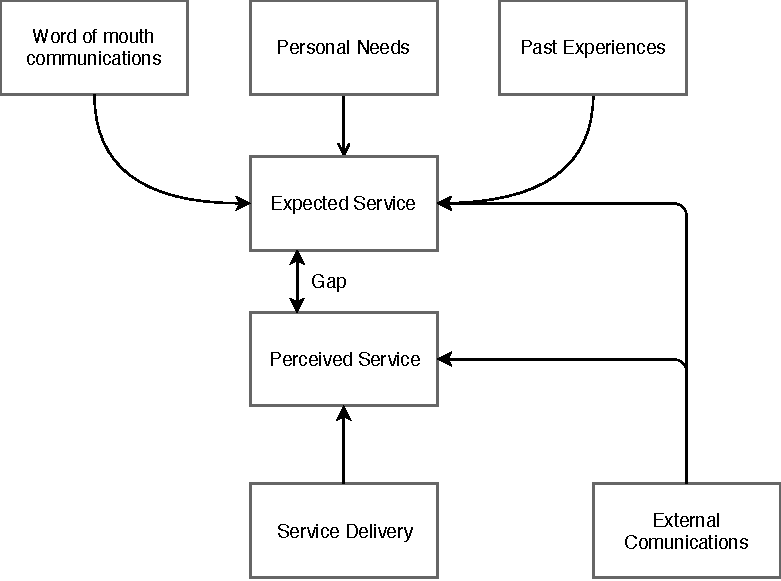
\includegraphics[width=1.00\textwidth]{expected_service.pdf}
	\caption[Factoren die bijdragen tot de verwachtingen van de gebruiker]{Factoren die bijdragen tot de verwachtingen van de gebruiker}
	\label{fig:expectedserviceperceivedservice}
\end{figure}

Tijdens dit onderzoek zullen we zowel de \foreign{service delivery} als \foreign{perceived service} proberen vergelijken tussen de twee technieken. Door deze vergelijking zullen we kunnen vaststellen of Linked Connections een betere user-perceived performance biedt, zowel absoluut als relatief ten opzichte van de werkelijke performance.

Een diepgaand onderzoek over de verwachte service valt buiten het bereik van deze masterproef. We zullen echter wel bondig de verwachtingen van gebruikers ondervragen, op vlak van dataverbruik, offline functionaliteit, en privacy, gezien deze drastisch verschillen bij Linked Connections ten opzichte van meer traditionele API's.

\section{Objectieve metingen}

Met objectieve metingen zullen we de werkelijke performance van elke API vastleggen. Ook zullen we het dataverbruik en batterijverbruik van beide technieken aan de hand van deze metingen trachten te bepalen.

Aangezien het onmogelijk is om automatisch volledige zoekopdrachten uit te voeren door de applicatie zonder de benodigde tijd te beïnvloeden, en aangezien de benodigde tijd om te renderen een constante is die gelijk is voor alle implementaties, zal er rechtstreeks op de API implementatie getest worden, net zoals de API normaal gezien gebruikt wordt. Het uittekenen van de resultaten op het scherm is een constante, welke verwaarloosbaar klein is in vergelijking met de tijd benodigd voor het ophalen van resultaten.

Om te voorkomen dat de keuze van de geteste stations of routes de objectieve metingen vertekent, zullen we de opzoekingen van echte gebruikers gebruiken. Hiervoor gebruiken we de log data van api.irail.be, die publiek beschikbaar zijn\footnote{https://gtfs.irail.be/logs}. Door deze \foreign{queries} opnieuw af te spelen op de applicaties kunnen we een zo goed mogelijk beeld krijgen van de werkelijke prestaties.

Objectief zullen we proberen om volgende gegevens vast te leggen
\begin{itemize}
	\item de gemiddelde tijd om alle data van de server te halen
	\item de gemiddelde tijd tussen zoekopdracht en weergave van het eerste resultaat
	\item de gemiddelde tijd tussen zoekopdracht en weergave van de eerste tien resultaten
	\item de gemiddelde hoeveelheid data die verzonden en ontvangen wordt
	\item het gemiddelde processorgebruik van het toestel
	\item het gemiddelde batterijgebruik van het toestel
\end{itemize}

Hiertoe zullen we gebruikmaken van een HTC 10 en een HTC One. Dit zijn twee smartphones in een zeer verschillende klasse op vlak van hardware én software. De verschillen tussen beide toestellen worden verduidelijkt in tabel~\ref{tab:testdevices}
\begin{table}[ht]
	\begin{tabular}{| c | c | c |}
		\hline
		Kenmerk & HTC One (M7) & HTC 10 \\
		\hline
		Besturingssysteem & Android 5.0 & Android 8.0 \\
		Processor & Qualcomm Snapdragon 600 & Qualcomm Snapdragon 820\\
		& (4x Krait 1,7GHz) & (4x Kryo 2,2GHz) \\
		Werkgeheugen & 2GB & 4GB \\
		Wi-Fi & 802.11ac & 802.11ac \\
		\hline
		Antutu Benchmark & 31.447 (mediaan)  & 133.791 (top 10\%) \\
		\hline
	\end{tabular}
	\caption[Specificaties van de toestellen gebruikt voor testen]{De specificiaties van gebruikte testtoestellen.}
	\label{tab:testdevices}
\end{table}

Benchmarks zijn synthetische metingen, en puur ter indicatie. Zo scoren typische budgettoestellen zoals de Motorola Moto G (1st gen), Motorola Moto G (3rd gen) en Nokia 3 respectievelijk 17.223, 21.000 en 26.500 punten op dezelfde AnTuTu benchmark, waarmee ze iets lager uitkomen dan de HTC One. Deze toestellen zijn instapmodellen uit 2013 tot nu. Een modern toestel van €200, zoals de Nokia 5, scoort 40.000, en komt daarmee al ruim boven de HTC One uit op vlak van prestaties. De HTC One is hierdoor geschikt om de prestaties te testen op oude en low-end smartphones.

Aan de andere kant is er de HTC 10, welke een gelijkaardige score behaalt als de Nokia 7 (103.000) en Samsung Galaxy S7 (157.000), en een (aanzienlijk) lagere score dan de Nokia 8 (208.000) of Samsung Galaxy S8 (201.000). Deze smartphone is dus geschikt om de prestaties om te testen voor duurdere mid-range toestellen of oudere high-end toestellen. Recentere high-end toestellen presteren aanzienlijk beter, oudere of goedkopere mid-range toestellen vallen tussen de HTC One en HTC 10 in. 

Zoals eerder vermeld zullen de opzoekingen van echte gebruikers worden gebruikt om te voorkomen dat het onderzoek vertekend wordt. In dit geval werden de opzoekingen op 2 mei 2018 gebruikt.

Voor alle tests werd gebruik gemaakt van de HTC 10 of HTC One zoals besproken in hoofdstuk~\ref{chap:onderzoek}, verbonden met internet via wifi (ping 26ms, downloadsnelheid 42mbps, uploadsnelheid 9mbps). Het toestel werd niet gebruikt tijdens de testen, en er werden geen achtergrondapplicaties uitgevoerd. De metingen werden automatisch uitgevoerd met behulp van \foreign{instrumented tests}. Metingen van Linked Connections (LC) gebruiken de LoganSquare JSON parser tenzij anders vermeld.

Voor de drie types resultaten zullen we telkens de metingen uit benchmarks bespreken, en de resultaten van user-testing. Bij de metingen zullen we telkens kort het effect van implementatiedetails bespreken, waarna we specifiek en gedetailleerd de prestaties van de huidige implementatie, op basis van de LoganSquare parser, bespreken. Uit deze metingen zullen we telkens trachten specifieke oorzaken van prestatieverschillen te achterhalen.

\section{Subjectieve metingen}

Gezien Linked Connections nog enkele belangrijke gegevens mist, zoals of een stop al dan niet afgeschaft is, en aan welk perron het voertuig zal aankomen of vertrekken, kunnen we dit systeem nog niet zelfstandig door gebruikers laten testen. Om rond deze beperking heen te werken zullen we in plaats hiervan begeleide user-tests uitvoeren met gebruikers, waarbij gebruikers gevraagd wordt om hun gebruikelijke opzoekingen te doen, per implementatie hun mening te geven, en vervolgens te bevragen welke variant hun voorkeur geniet, op vlak van snelheid, functionaliteit, en privacy.
We zullen ook zeer eenvoudig aftasten welke functionaliteit gebruikers het meest interessant vinden, zodat verder onderzoek zich hierop kan richten.

Door middel van een bevraging zullen we trachten een antwoord te vinden op volgende vragen:
\begin{itemize}
	\item Biedt offline informatie een meerwaarde voor gebruikers?
	\item Hecht de gebruiker belang aan privacy bij het gebruik van routeplanning apps? Zo ja, in welke mate?
	\item Heeft de gebruiker schrik om te veel mobiele data te verbruiken?
	\item Hecht de gebruiker belang aan dataverbruik bij het gebruik van routeplanning apps?
	\item Is de gebruiker tevreden met de snelheid van zijn huidige routeplanning app?
	\item Wat is voor een gebruiker belangrijk in routeplanning apps?
	\item Is de gebruiker geïnteresseerd in routeplanning op maat? Zo ja, welke aspecten spreken hem dan aan?
	\item Is de gebruiker geïnteresseerd in offline opzoekingen?
	\item Is de gebruiker geïnteresseerd in de mogelijke snelheid die Linked Connections biedt?
	\item Is de gebruiker geïnteresseerd in de volledige privacy die Linked Connections biedt?
\end{itemize}

Door middel van user-testing zullen we proberen om ook deze vragen te beantwoorden:
\begin{itemize}
	\item Ervaart de gebruiker een app die lokaal Linked Connections gebruikt als sneller dan een app die gebruikmaakt van een RPC API?
	\item Ervaart de gebruiker een app die lokaal Linked Connections gebruikt als sneller dan zijn huidige app?
\end{itemize}

Om een antwoord op bovenstaande vragen te vinden, werd een enquête opgebouwd. Deze exacte vraagstelling voor deze enquête is terug te vinden in bijlage~\ref{appendix:enquete}.
% !TeX spellcheck = nl_NL
\begin{savequote}[0.55\linewidth]
	``Inspirational quote''
	\qauthor{\textasciitilde Source}
\end{savequote}

\chapter{Resultaten}
\label{chap:resultaten}

Zoals eerder vermeld in hoofdstuk~\ref{chap:onderzoek}, worden opzoekingen van echte gebruikers gebruikt om te voorkomen dat het onderzoek vertekend wordt. In dit geval werden de opzoekingen op 2 mei 2018 gebruikt.

Voor de alle tests werd gebruik gemaakt van de HTC 10 of HTC One zoals besproken in hoofdstuk~\ref{chap:onderzoek}, verbonden met internet via wifi (ping 26ms, downloadsnelheid 42mbps, uploadsnelheid 9mbps). Het toestel werd niet gebruikt tijdens de testen, en er werden geen achtergrondapplicaties uitgevoerd. De metingen werden automatisch uitgevoerd met behulp van \foreign{instrumented tests}. Metingen van Linked Connections (LC) gebruiken de LoganSquare JSON parser tenzij anders vermeld.

Voor de drie types resultaten zullen we telkens de metingen uit benchmarks bespreken, en de resultaten van user-testing. Bij de metingen zullen we telkens kort het effect van implementatiedetails bespreken, waarna we specifiek en gedetailleerd de prestaties van de huidige implementatie, op basis van de LoganSquare parser, bespreken. Uit deze metingen zullen we telkens trachten specifieke oorzaken van prestatieverschillen te achterhalen.

Hierna worden telkens de ervaringen van gebruikers besproken. Dit omvat absolute ervaringen (zonder exact referentiepunt, maar tegenover de expected service zoals vermeld in hoofdstuk~\ref{chap:onderzoek}), maar ook de relatieve ervaringen tussen LC2Irail en Linked Connections, en de relatieve ervaringen tegenover de huidige applicatie van de gebruiker zullen besproken worden.

Tot slot zullen we nog kijken naar de uiteindelijke keuze van de gebruiker, en bespreken we ook de resultaten van de enquete. Een globale interpretatie van de resultaten volgt in hoofdstuk~\ref{chap:interpretatie}.

\section{Liveboards}
\subsection{Metingen}
\begin{figure}[h]
	\centering
	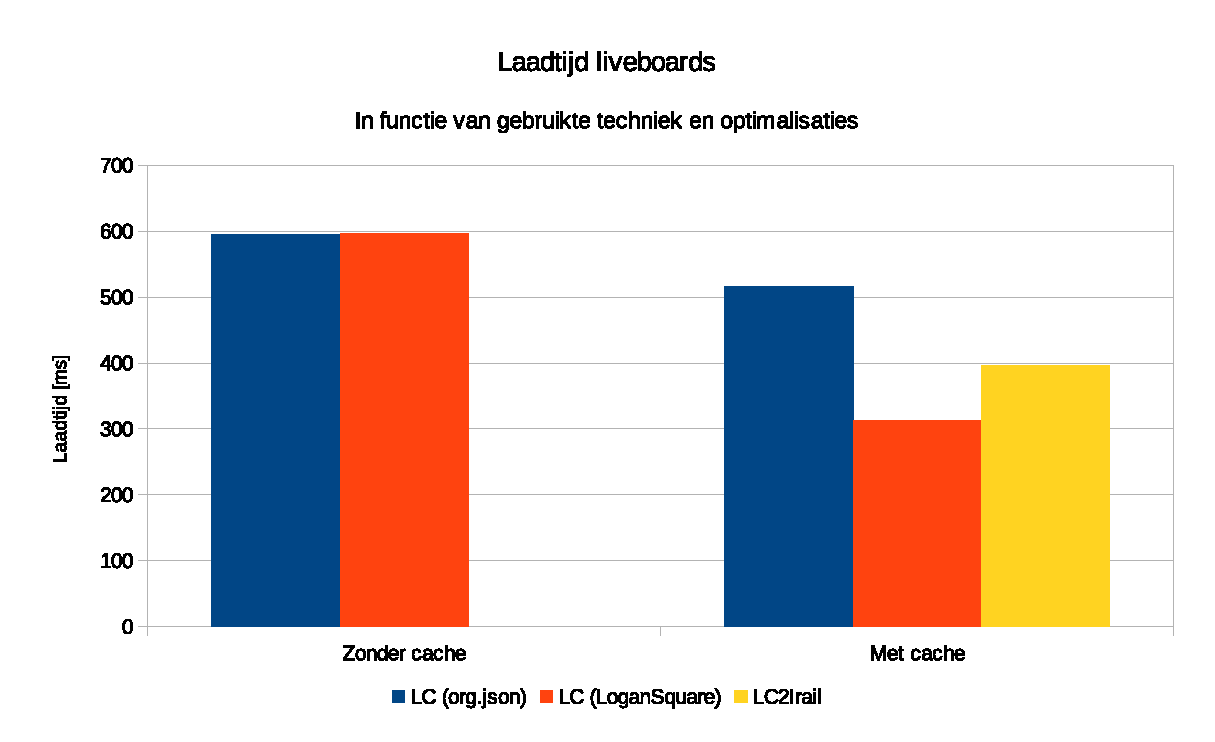
\includegraphics[width=0.80\textwidth]{Optimalisaties_liveboards.eps}
		\caption[Gemeten laadtijd liveboards]{De gemiddelde gemeten laadtijd voor liveboards gebruikmakend van een HTC 10 voor 262 opzoekingen gebaseerd op de iRail logs. }
	\label{fig:liveboardlabtest}
\end{figure}
%\begin{table}[h]
%	\begin{tabular}{| c | c | c | c | c | c |}
%		\hline
%		Variant & parser & cache & minimaal (ms) & gemiddelde (ms) & maximaal (ms)\\
%		\hline
%		LC op toestel & org.json & nee & 302 &  595 &  3471 \\
%		LC op toestel & org.json & ja & 409 &  516  &  3599 \\
%		LC op toestel & LoganSquare & nee & 392 & 597 & 2027 \\
%		LC op toestel & LoganSquare & ja  & 166 & 313 & 3428 \\
%		
%		LC op server &&&  232 & 397 &  1421\\
%		\hline
%	\end{tabular}
%	\caption[Gemeten laadtijd liveboards]{De gemeten laadtijd voor het eerste resultaat liveboards gebruikmakend van een HTC 10 voor 262 opzoekingen gebaseerd op de iRail logs. }
%	\label{tab:liveboardlabtest}
%\end{table}

Zoals eerder vermeld vergelijken we eerst kort verschillende implementaties van Linked Connections. In grafiek~\ref{fig:liveboardlabtest} zijn de gemiddelde resultaten zichtbaar van een benchmark waarbij 262 stations opgezocht werden, ongeveer 5\% van de opzoekingen door gebruikers op 2 mei 2018. Telkens is de minimale, gemiddelde en maximale responstijd gemeten. Dit zowel gebruikmakend van de standaard (\foreign{org.json}) JSON parser en gebruikmakend van de \foreign{LoganSquare} parser. Ook werd de test herhaald met cache in- en uitgeschakeld, om zo het effect hiervan te meten. Tot slot werd dezelfde test herhaald gebruikmakend van data afkomstig van de LC2Irail web applicatie om een vergelijking tussen de twee methodes te kunnen maken. Deze cijfers geven slechts een indicatie van de snelheid -- een volledige en diepgaande statistische analyse van de performantieverschillen tussen verschillende implementaties van dezelfde techniek valt wegens tijdsgebrek buiten het bereik van deze masterproef.

In deze cijfers is invloed van de cache duidelijk merkbaar. We zien wel een duidelijk verschil tussen de JSON parsers: terwijl bij gebruik van de \foreign{LoganSquare} parser de gemiddelde laadtijd bijna halveert, terwijl het effect van de cache bij het gebruik van de \foreign{org.json} parser veel kleiner is. Wanneer de cache uitgeschakeld is is het verschil tussen de parsers verwaarloosbaar. Dit is mogelijk te verklaren door het feit dat voor het tonen van vertrekken of aankomsten relatief weinig data nodig is: in de meeste gevallen volstaat een enkele Linked Connections pagina.

Om een exact beeld te vormen van de prestaties, zoeken we een duizendtal liveboards op. Hiervoor kiezen we elke vijfde opzoeking uit de iRail logs. Voor elk liveboard worden twintig resultaten geladen. De resultaten hiervan zijn zichtbaar in grafieken~\ref{fig:liveboardsDiefBest},~\ref{fig:liveboardsDiefAvg} en~\ref{fig:liveboardsDiefSlechtst}, respectievelijk voor het tiende, vijftigste en negentigste percentiel. Uit deze grafieken kunnen we duidelijke trends zien:

\begin{figure}[h]
	\centering
	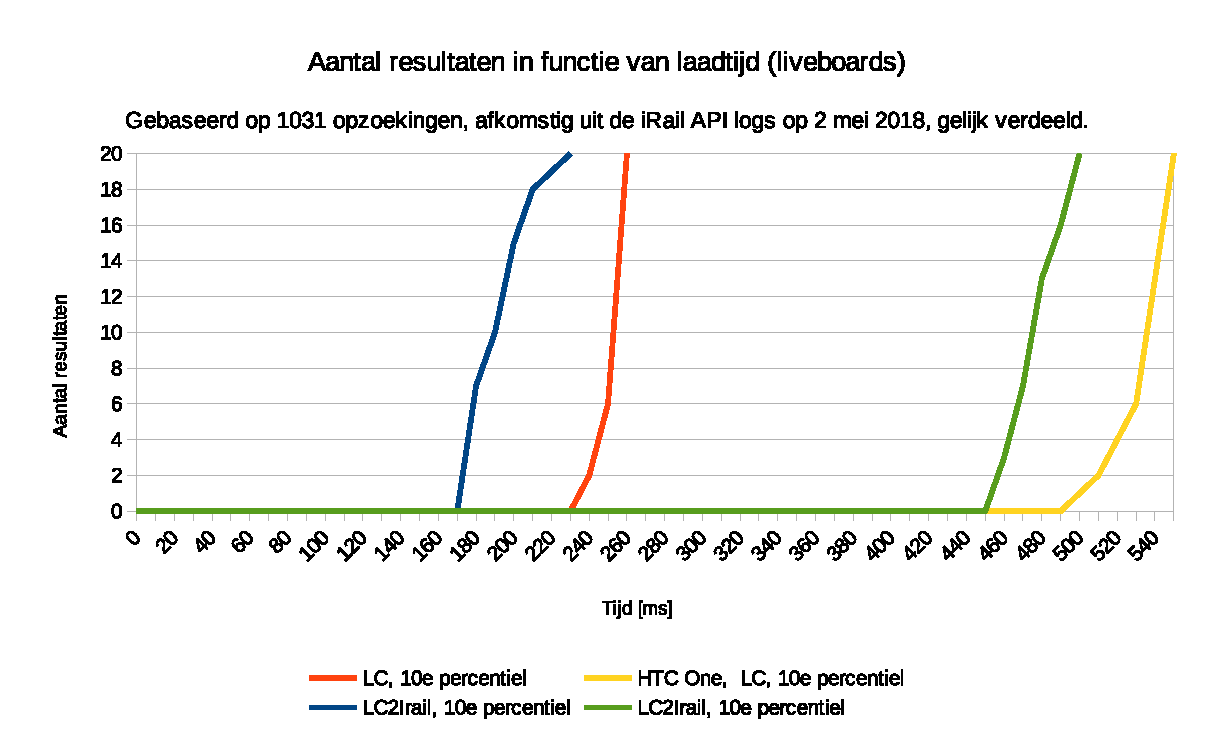
\includegraphics[width=1.00\textwidth]{dief_liveboards_best.eps}
	\caption[Aantal resultaten liveboards in functie van de tijd]{Het aantal resultaten in functie van de verlopen tijd.}
	\label{fig:liveboardsDiefBest}
\end{figure}

\begin{figure}[h]
	\centering
	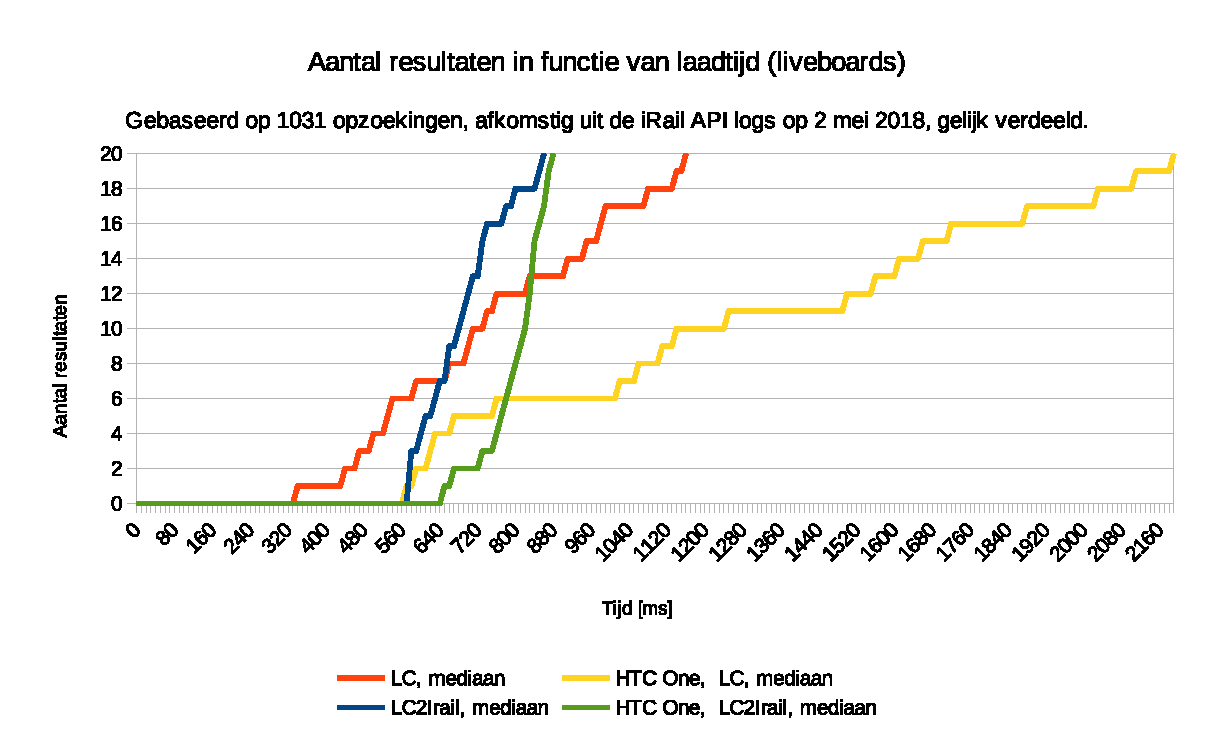
\includegraphics[width=1.00\textwidth]{dief_liveboards_gemiddeld.eps}
	\caption[Aantal resultaten liveboards in functie van de tijd]{Het aantal resultaten in functie van de verlopen tijd.}
	\label{fig:liveboardsDiefAvg}
\end{figure}

\begin{figure}[h]
	\centering
	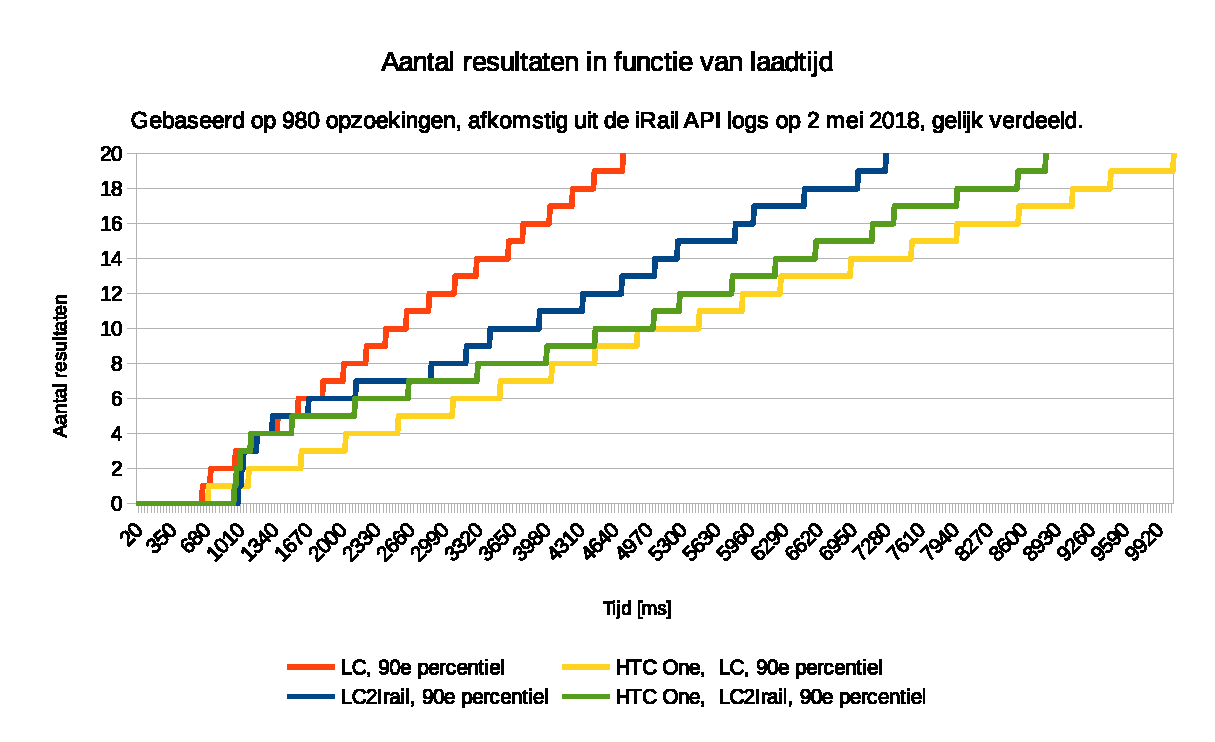
\includegraphics[width=1.00\textwidth]{dief_liveboards_slechtst.eps}
	\caption[Aantal resultaten liveboards in functie van de tijd]{Het aantal resultaten in functie van de verlopen tijd.}
	\label{fig:liveboardsDiefSlechtst}
\end{figure}


\begin{itemize}
    \item In de snelste gevallen is de serverimplementatie sneller. Hiervoor kunnen we verschillende oorzaken aanwijzen: 
	\begin{itemize}
		\item De serverimplementatie kan resultaten op een specifieke vraag cachen, terwijl de lokale implementatie deze steeds zal herberekenen vanaf Linked Connections pagina's. Voor veel voorkomende zoekopdrachten, zoals populaire stations, kan de server ook Linked Connections pagina's cachen.
		\item De serverimplementatie hoeft minder data te versturen. Ook het parsen van het antwoord gaat sneller, gezien slechts een kleine hoeveelheid data verwerkt moet worden en er verder geen berekeningen moeten gebeuren.
	\end{itemize}

	\item Terwijl in de snelste gevallen de serverimplementatie sneller is, is dit verschil beperkt tot ongeveer 60 milliseconden voor het eerste resultaat. Dit ligt zeer kort bij een verschil van 10\%, wat in deze ordegrootte moeilijk onderscheidbaar is voor gebruikers~\citep{miller68}. %TODO CITE Weber-Fechner Law
	
	\item Wanneer we naar de mediane performantie kijken, is Linked Connections duidelijk sneller voor de eerste resultaten. Dit snelheidsverschil is aanzienlijk, en hoogstwaarschijnlijk vooral te wijten aan het feit dat Linked Connections volledige ondersteuning biedt voor incrementele resultaten, waarbij de server meestal meerdere pagina's zal overlopen voor een  antwoord gegeven wordt. Dit is te zien aan de steile curves voor LC2Irail, waar de curves voor LC gekenmerkt worden door een minder sterke stijging. 
	
	Anderzijds is er bij Linked Connections sprake van een \foreign{overhead} door het laden van te veel data. Voor stations met weinig vertrekken, of tijdens piekuren, kan het hierdoor meer moeite kosten om Linked Connections te verwerken. We vermoeden dat dit contrast met de korte, informatiedichte antwoorden van de RPC API zorgt voor het trager laden van resultaten. We zien dat hoe sneller het toestel, hoe langer Linked Connections het snelst blijft. Dit bevestigt de hypothese dat het verwerken van Linked Connections pagina's aan de oorzaak ligt. Ook blijft het verschil tussen Linked Connections en LC2Irail beperkt op de HTC 10, terwijl dit verschil aanzienlijk oploopt op de tragere HTC One.
	
	\item In alle gevallen is er een sterke gelijkenis tussen de curves voor LC2Irail op het HTC 10 toestel en het HTC One toestel. Deze zijn enkel een relatief kleine afstand in tijd verschoven, wat verklaart kan worden door de lage belasting voor het mobiele toestel wanneer een RPC API gebruikt wordt.

	\item Het verschil in laadtijd tussen Linked Connections op de twee toestellen loopt lineair op met de benodigde laadtijd om resultaten te laden. Zo zien we dat in het slechtste geval dubbel zoveel tijd benodigd is op de HTC One in vergelijking met de HTC 10. Dit is een sterke indicatie dat de performantie van Linked Connections afhankelijk is van het gebruikte toestel.
\end{itemize}

\begin{figure}[h]
	\centering
	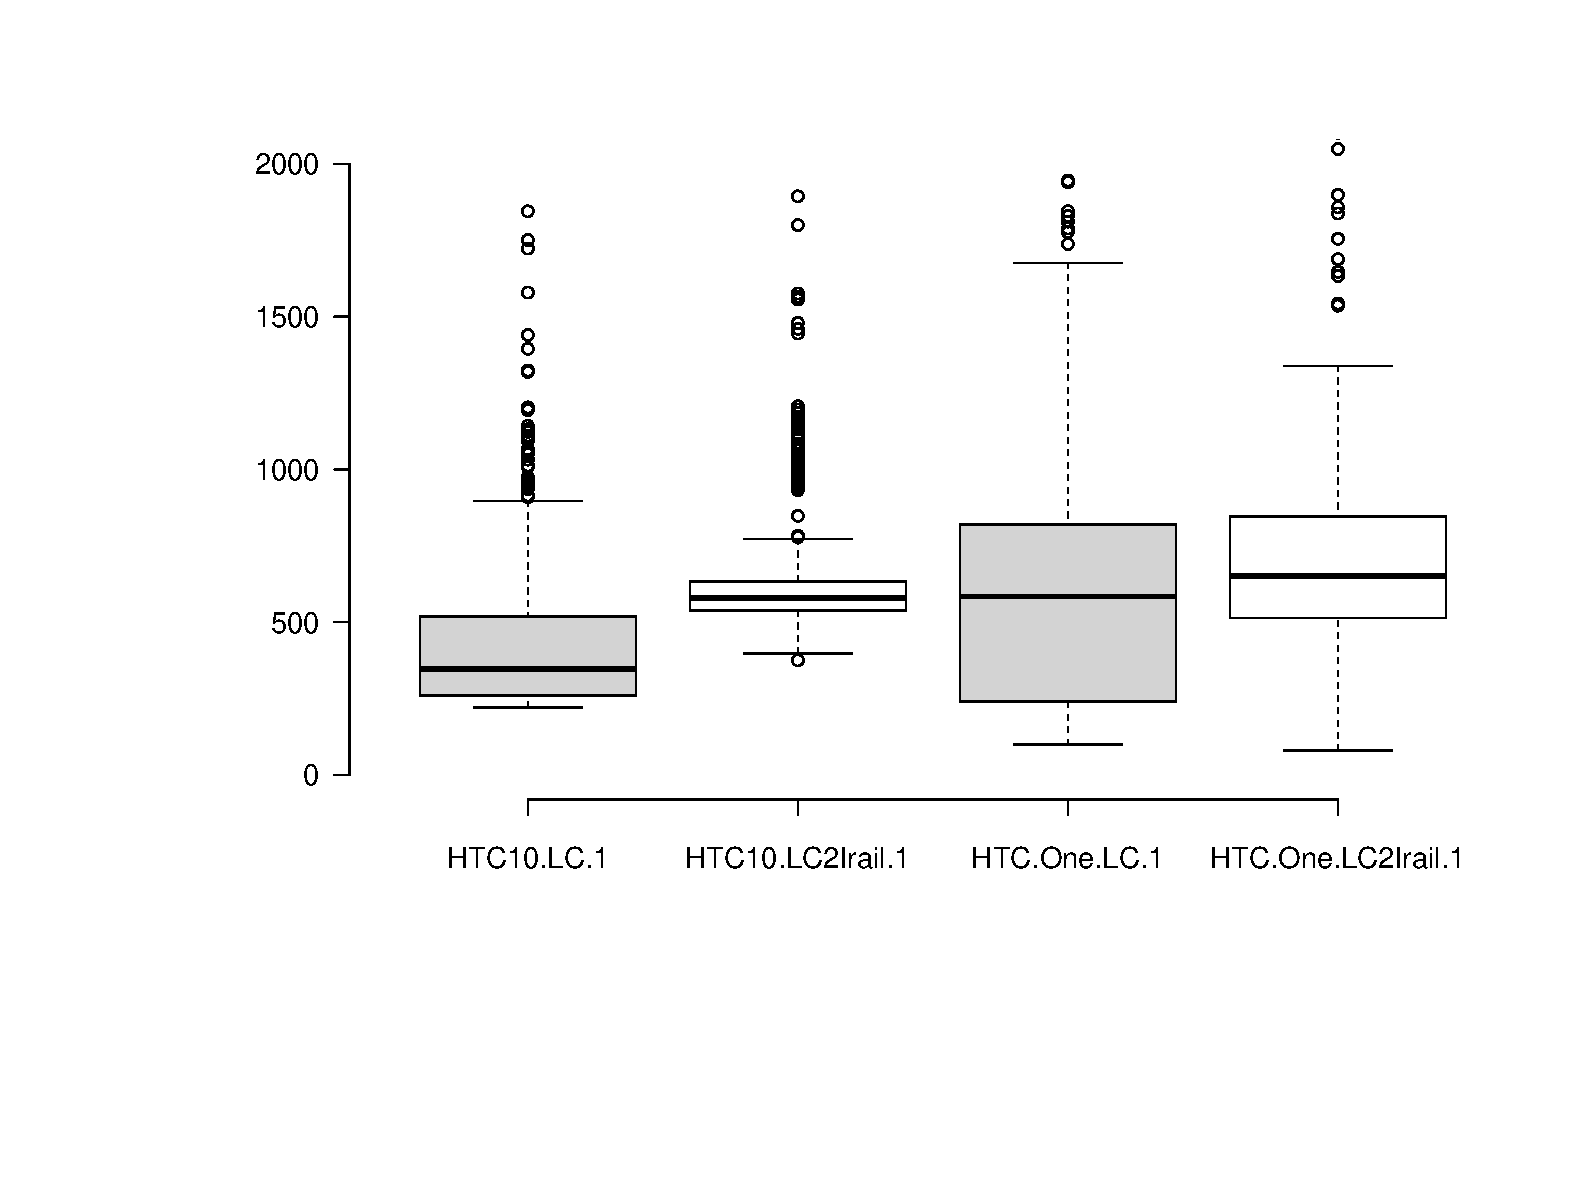
\includegraphics[width=1.00\textwidth]{boxplot_liveboards_1.eps}
	\caption[Laadtijd eerste resultaat liveboard in functie van toestel en technologie]{Laadtijd eerste resultaat liveboard in functie van toestel en technologie.}
	\label{fig:liveboardsBoxplot1}
\end{figure}

\begin{figure}[h]
	\centering
	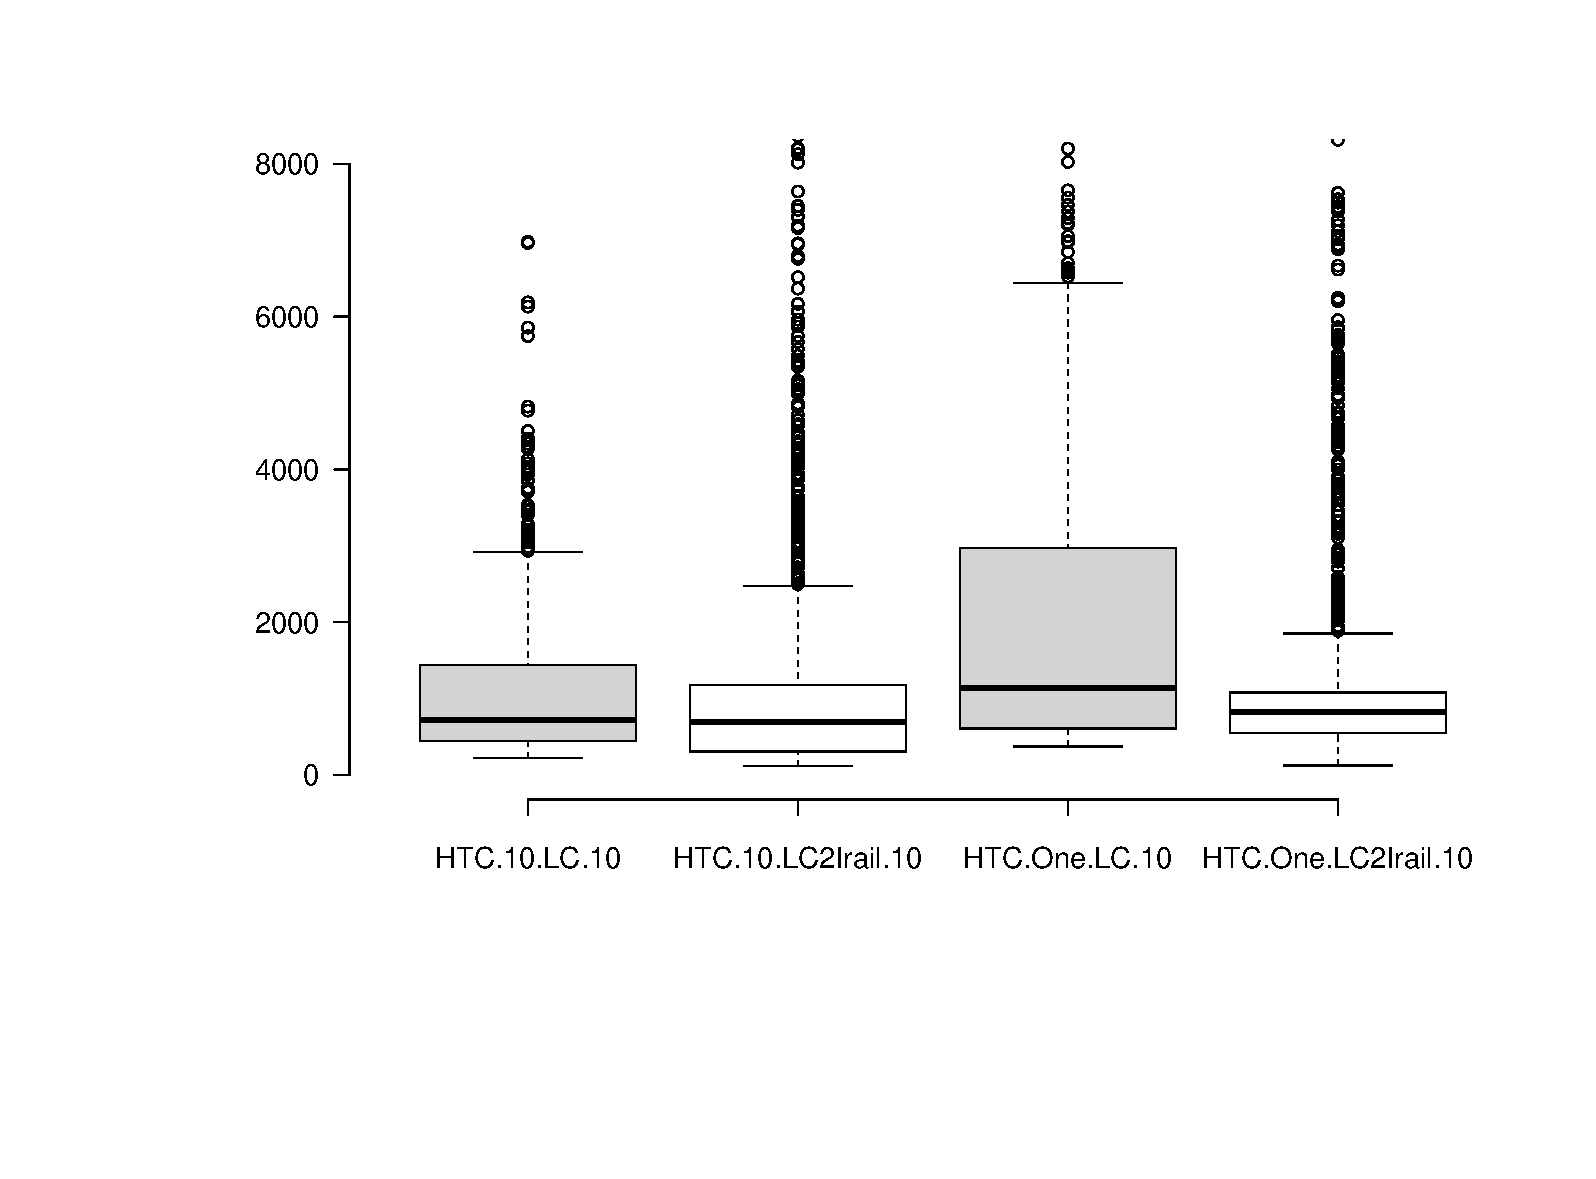
\includegraphics[width=1.00\textwidth]{boxplot_liveboards_10.eps}
	\caption[Laadtijd tiende resultaat liveboard in functie van toestel en technologie]{Laadtijd tiende resultaat liveboard in functie van toestel en technologie.}
	\label{fig:liveboardsBoxplot10}
\end{figure}

Wanneer we nu naar de spreiding van de laadtijden kijken, zichtbaar in figuur~\ref{fig:liveboardsBoxplot1} voor het eerste resultaat en figuur~\ref{fig:liveboardsBoxplot10} voor het tiende resultaat, zien we ook hier duidelijke verschillen tussen de verschillende methodes. Telkens levert LC2Irail een dichtere verdeling op dan LC, waarbij Linked Connections enkel sneller is voor het eerste resultaat op de HTC 10. Voor het eerste resultaat op de HTC One, en het tiende resultaat op de HTC 10, zijn beide implementaties volgens de wet van Weber-Fechner niet te onderscheiden op de mediaan.

In deze grafieken zijn ook de verschillen tussen toestellen enorm interessant. Zo zien we dat bij gebruik van een RPC API de mediaan van de laadtijd ongeveer gelijk is tussen verschillende toestellen, en de interkwartielafstand relatief klein is, wat op een kleine spreiding en dus consistente resultaten per toestel duidt. De mediaan voor beide toestellen ligt respectievelijk op 578 en 650 milliseconden voor het eerste resultaat. Volgens de wet van Weber-Fechner is dit onmerkbaar voor gebruikers. Ook het eerste kwartiel ligt kort genoeg bij elkaar om niet merkbaar te zijn. Ondanks dat we boven de mediaan zien dat opzoekingen via LC2Irail op de HTC One meer tijd vergen, is onder de mediaan voor gebruikers geen verschil merkbaar. Deze zeer consistente ervaring over toestellen is zeer wenselijk voor routeplanning applicatie. Voor het tiende resultaat neemt het verschil tussen de toestellen toe, waarbij gebruikers een verschil zullen merken tussen de LC2Irail implementatie op verschillende toestellen.

Bij gebruik van Linked Connections zien we duidelijke verschillen tussen de mediaan van de laadtijd bij verschillende toestellen. Ook de interkwartielafstand varieert tussen toestellen: zo is een ouder toestel niet enkel trager, maar is ook de spreiding veel groter, en zijn de resultaten dus minder consistent op oudere (tragere) toestellen. Anderzijds is Linked Connections in de meeste gevallen wel duidelijk sneller dan LC2Irail op de HTC 10.

Een eigenaardigheid is dat de minima voor de HTC One telkens lager liggen. Dit wordt vermoedelijk veroorzaakt door verschillende Android versies, met een verschillende aanpak op vlak van asynchrone scheduling.

\subsection{Ervaringen}
Wanneer we nu naar de ervaringen van gebruikers gaan kijken, stemmen deze ongeveer overeen met wat we zouden verwachten na evaluatie van de metingen.

Zoals we in figuren~\ref{fig:liveboardsBoxplot1} en~\ref{fig:liveboardsBoxplot10} konden zien blijkt uit testen dat de performantie van LC2Irail consistenter is, zowel in de vorm van een kleinere spreiding van de resultaten op eenzelfde toestel, als in de vorm van kleinere verschillen tussen toestellen. Ook bij de gebruikerservaring zien we dit terugkomen. Wanneer de ervaren snelheid wordt uitgezet in een boxplot per techniek, zichtbaar in figuur~\ref{fig:liveboardsUx}, zien we net als bij de testen dat voor LC2Irail een heel consistente beoordeling wordt gegeven, terwijl deze voor Linked Connections veel meer uitgespreid, én iets lager ligt.

\begin{figure}[h]
	\centering
	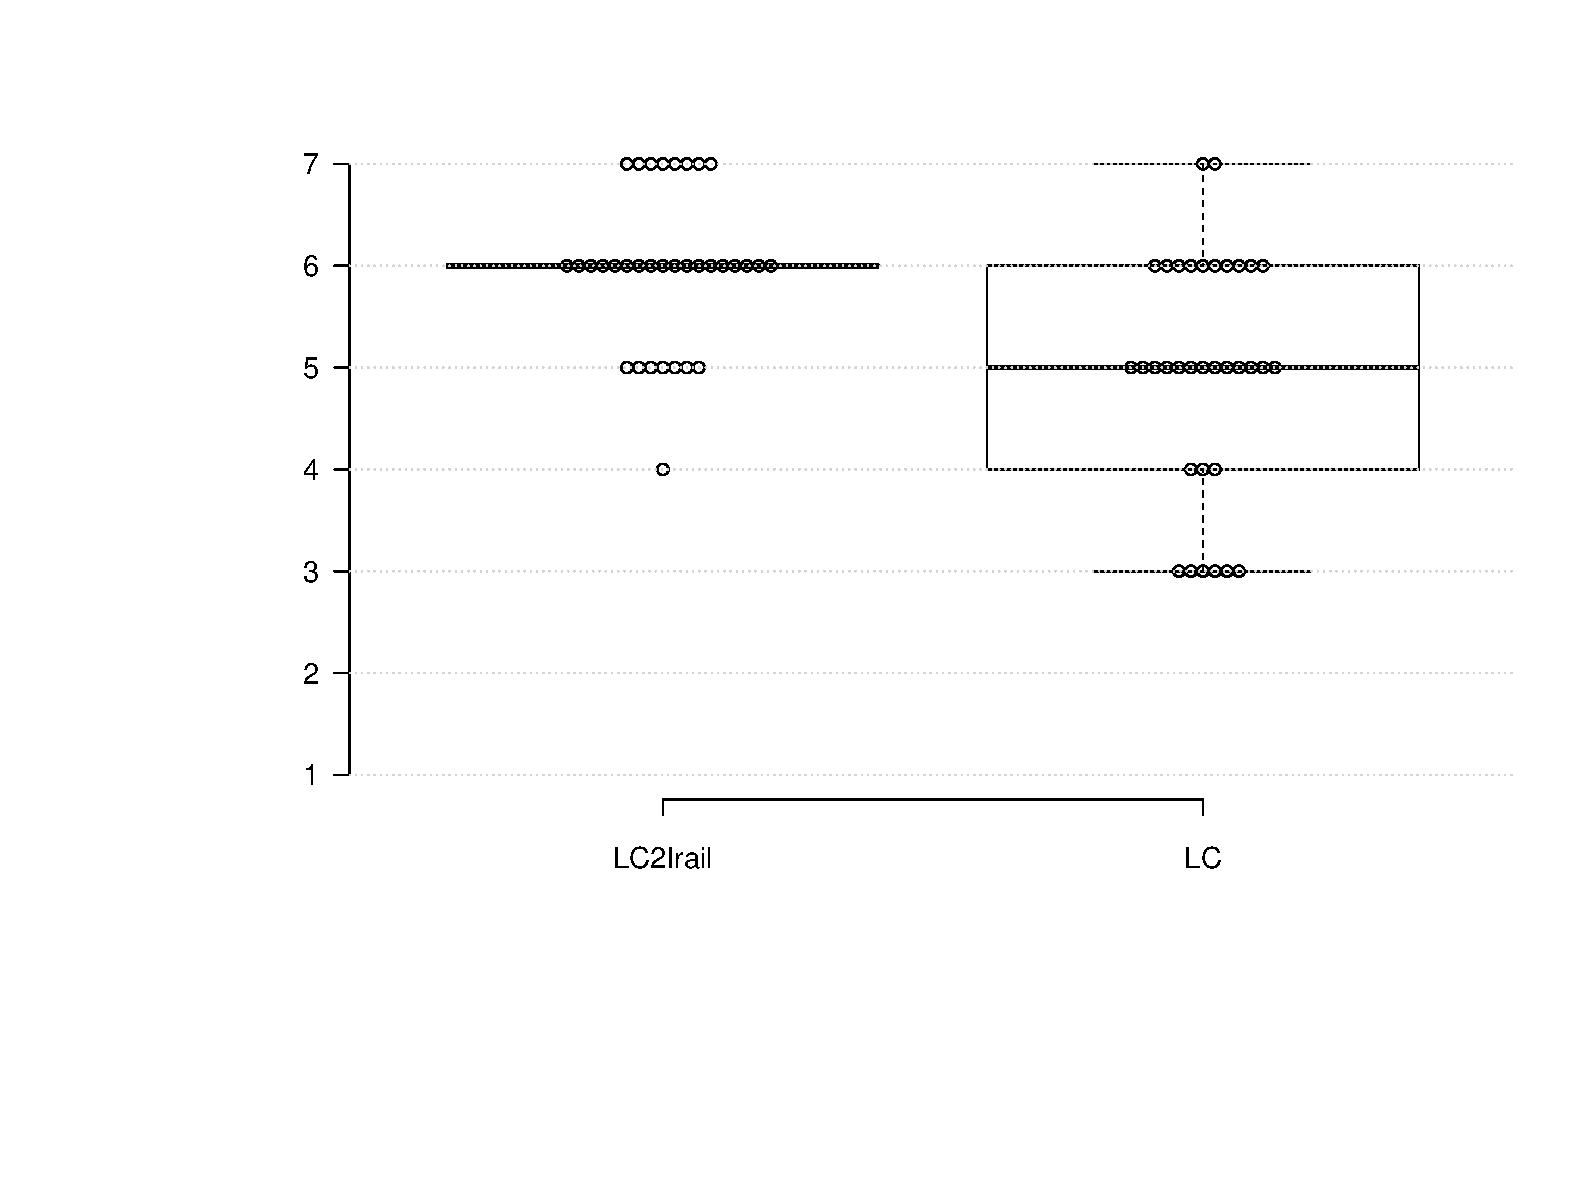
\includegraphics[width=0.80\textwidth]{boxplot_liveboards_ux.eps}
	\caption[Ervaren snelheid van liveboards]{De ervaren snelheid op een schaal 1-7 van vertrekken en aankomsten voor LC2Irail en Linked Connections, gebaseerd op 17 user-tests.}
	\label{fig:liveboardsUx}
\end{figure}

Hoewel 12 van de 17 testpersonen Linked Connections als redelijk tot extreem snel ervaart, zijn er slechts twee personen die Linked Connections sneller ervaren dan LC2Irail. De ervaringen en uiteindelijk keus op basis van snelheid is zichtbaar in figuur~\ref{fig:alluvialUserChoicesLiveboards}. Het is duidelijk zichtbaar dat de ervaringen voor Linked Connections veel gemengder zijn dan de ervaringen voor LC2Irail. Er zijn zowel mensen die Linked Connections sneller, even snel of trager ervaren. 

\begin{figure}[ht]
	\centering
	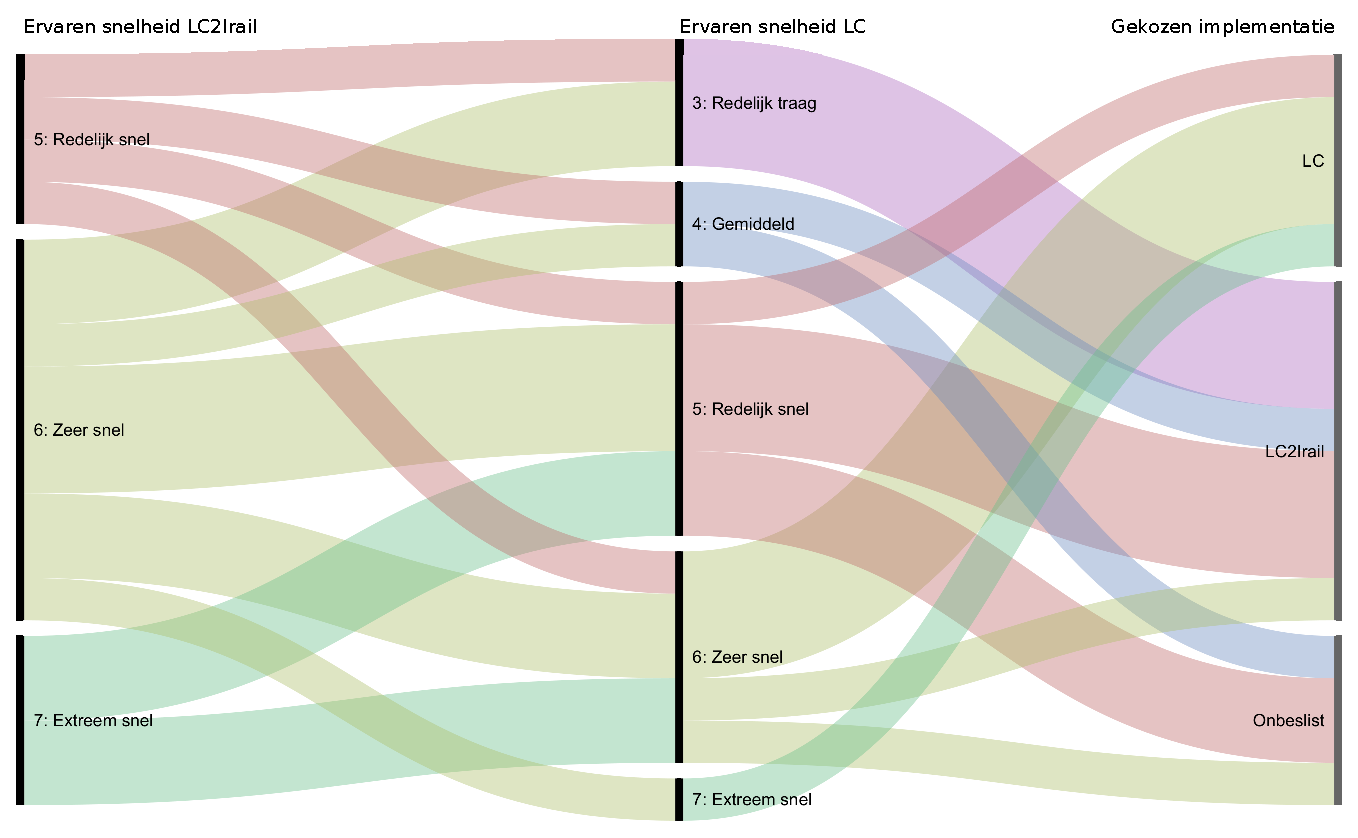
\includegraphics[width=1.00\textwidth]{alluvial_user_choice_departures.eps}
	\caption[Door gebruikers gekozen implementatie voor liveboards]{Verbanden tussen de door gebruikers gekozen implementaties voor liveboards. }
	\label{fig:alluvialUserChoicesLiveboards}
\end{figure}

Alle testpersonen werden expliciet gevraagd welke implementatie ze als sneller ervoeren. Hierbij waren de antwoorden verdeeld: acht personen kozen de Linked Connections, vier personen hadden geen mening, en vijf personen kozen LC2Irail variant. Het is moeilijk om hier onmiddelijk conclusies uit te trekken. Om deze reden zullen we in hoofdstuk~\ref{chap:interpretatie} de resultaten algemener bespreken. Wel kunnen we zeggen dat gebruikerservaringen zeer gemengd zijn voor Linked Connections, en zal Linked Connections zoiezo niet voor de volledige populatie sneller zijn.

Wanneer we gaan kijken naar de verschillen tussen de JSON parsers, blijkt dat beide parsers ongeveer even goed presteren in de ogen van de testers. Respectievelijk 5 op 7 en 7 op 10 testers zijn neutraal of tevreden, en bij beide varianten is er telkens een tester neutraal. Deze vergelijking is echter slechts een indicatie, en is door te kleine steekproeven ongeschikt om te veralgemenen naar een grotere populatie.

Wanneer echter gekeken wordt naar de gemeten prestatieverschillen tussen beide JSON parsers tijdens de usertests, zien we een duidelijk verschil, waarbij het 90e percentiel van de laadtijd onder de LoganSquare parser lager ligt dan de mediane laadtijd van de org.json parser. Dit verschil lijkt echter geen invloed te hebben op de ervaringen van gebruikers, vermoedelijk omdat men beide reeds als performant genoeg ervaart. % TODO: Hoe groot procentueel verschil?

\begin{figure}[ht]
	\centering
	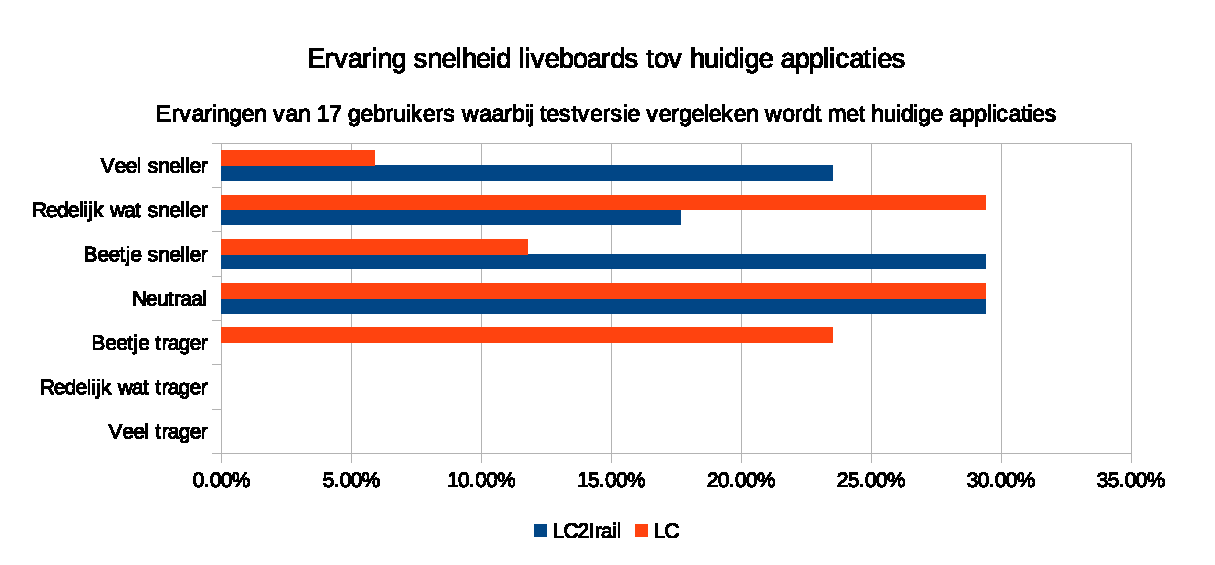
\includegraphics[width=1.00\textwidth]{userdata_liveboards_currentapp.eps}
	\caption[Door gebruikers ervaren snelheid liveboards tov huidige apps]{De door 17 gebruikers ervaren snelheid liveboards ten opzichte huidige apps }
	\label{fig:relativePerceptionLiveboards}
\end{figure}

Als tot slot gevraagd wordt om de snelheid te vergelijken met de applicatie die de gebruiker op dit moment gebruikt, zichtbaar in figuur~\ref{fig:relativePerceptionLiveboards} , komen beide apps er goed uit. LC2Irail scoort hier zeer goed, en ondanks dat Linked Connections iets minder goed scoort dan LC2Irail, geven slechts 2 gebruikers aan Linked Connections trager te ervaren dan hun huidige applicatie.

\section{Routes}

\subsection{Metingen}
\begin{figure}[h]
	\centering
	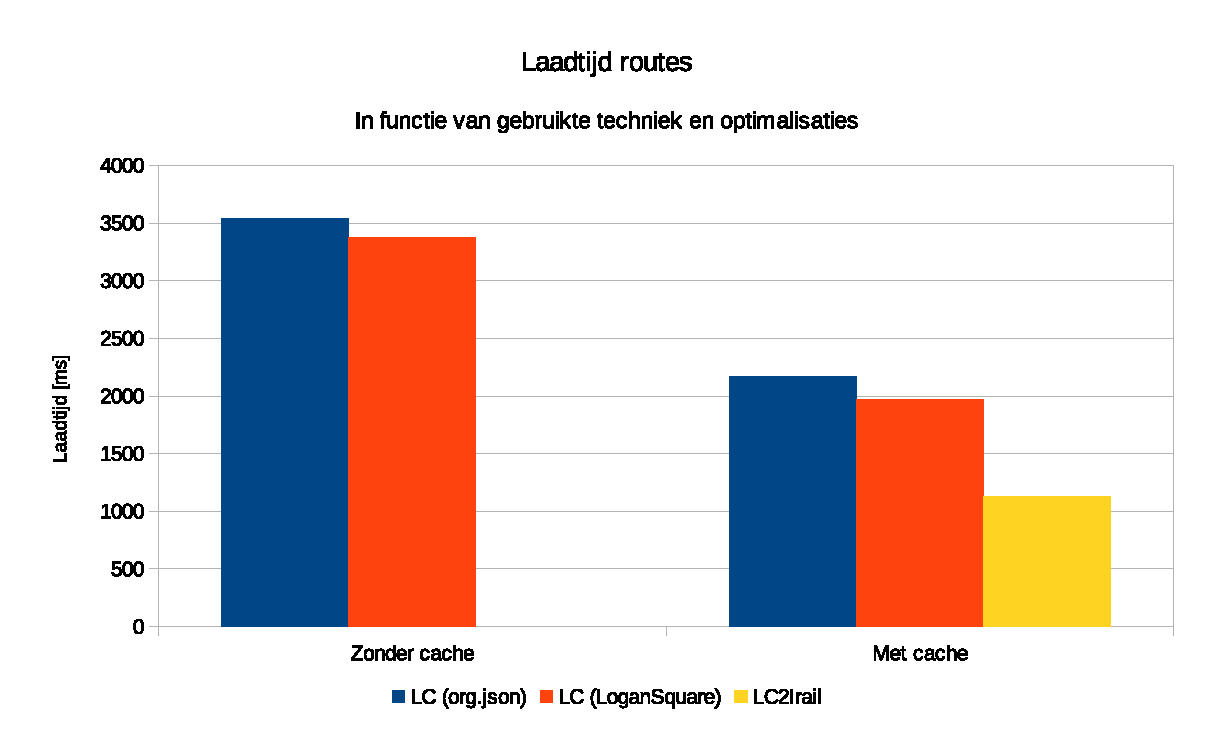
\includegraphics[width=0.80\textwidth]{Optimalisaties_routes.eps}
	\caption[Gemeten laadtijd routes]{De gemiddelde gemeten laadtijd voor routes gebruikmakend van een HTC 10 voor 779 opzoekingen gebaseerd op de iRail logs.}
	\label{fig:routelabtest}
\end{figure}
%\begin{table}[h]
%	\begin{tabular}{| c | c | c | c | c | c |}
%		\hline
%		Variant & parser & cache & minimaal (ms) & gemiddelde (ms) & maximaal (ms)\\
%		\hline
%		LC op toestel & org.json & nee & 401 & 3539 & 8531\\
%		LC op toestel & org.json & ja & 221 & 2172 & 6960 \\
%		LC op toestel & LoganSquare & nee &  386 & 3374 & 7554 \\
%		LC op toestel & LoganSquare & ja  & 233 & 1973 & 7640 \\
%		
%		LC op server &&&  27 & 1126 & 3374\\
%		\hline
%	\end{tabular}
%	\caption[Gemeten laadtijd routes]{De gemeten laadtijd voor routes gebruikmakend van een HTC 10 voor 779 opzoekingen gebaseerd op de iRail logs.}
%	\label{tab:routelabtest}
%\end{table}

Ook voor routes zullen we eerst kort de relatieve prestaties van verschillende implementaties bespreken. In grafiek~\ref{fig:routelabtest} zijn de gemiddelde resultaten zichtbaar van een benchmark waarbij 779 routes opgezocht werden, ongeveer 5\% van de opzoekingen door gebruikers op 2 mei 2018. Telkens is de minimale, gemiddelde en maximale responstijd gemeten. Dit zowel gebruikmakend van de standaard JSON parser (\foreign{org.json}) en gebruikmakend van de \foreign{LoganSquare} parser. Ook werd de test herhaald met cache in- en uitgeschakeld, om zo het effect hiervan te meten. Tot slot werd dezelfde test herhaald gebruikmakend van data afkomstig van de LC2Irail web applicatie om een vergelijking tussen de twee methodes te kunnen maken. Deze cijfers geven slechts een indicatie van de snelheid - een volledige en diepgaande statistische analyse van de performantieverschillen tussen verschillende implementaties van dezelfde techniek valt wegens tijdsgebrek buiten het bereik van deze masterproef.

Net zoals bij liveboards is ook hier de invloed van de cache duidelijk merkbaar. Dit valt te verklaren door de grote hoeveelheden data die verwerkt moeten worden, waarbij het cruciaal is dat deze niet steeds opnieuw gedownload wordt. Vergeleken met dezelfde analyse voor Liveboards (figuur~\ref{fig:liveboardlabtest}), zien we hier een minder groot verschil tussen de parsers. Dit komt mogelijk door de grotere impact van de verdere algoritmes, waardoor de invloed van parsing verkleint. Het algoritme om de data tot routes te verwerken is het zwaarst van de drie endpoints. %TODO: remove LC2Irail from graph

Om ook hier een exact beeld te vormen van de prestaties, maken we ook hier een duizendtal opzoekingen. Hiervoor kiezen we telkens de vijfde opzoeking uit de iRail logs. Voor elke route wordt gepoogd 10 resultaten geladen. De resultaten hiervan zijn zichtbaar in grafieken~\ref{fig:routesDiefBest},~\ref{fig:routesDiefAvg} en~\ref{fig:routesDiefSlechtst}, respectievelijk voor het tiende, vijftigste en negentigste percentiel.

\begin{figure}[h]
	\centering
	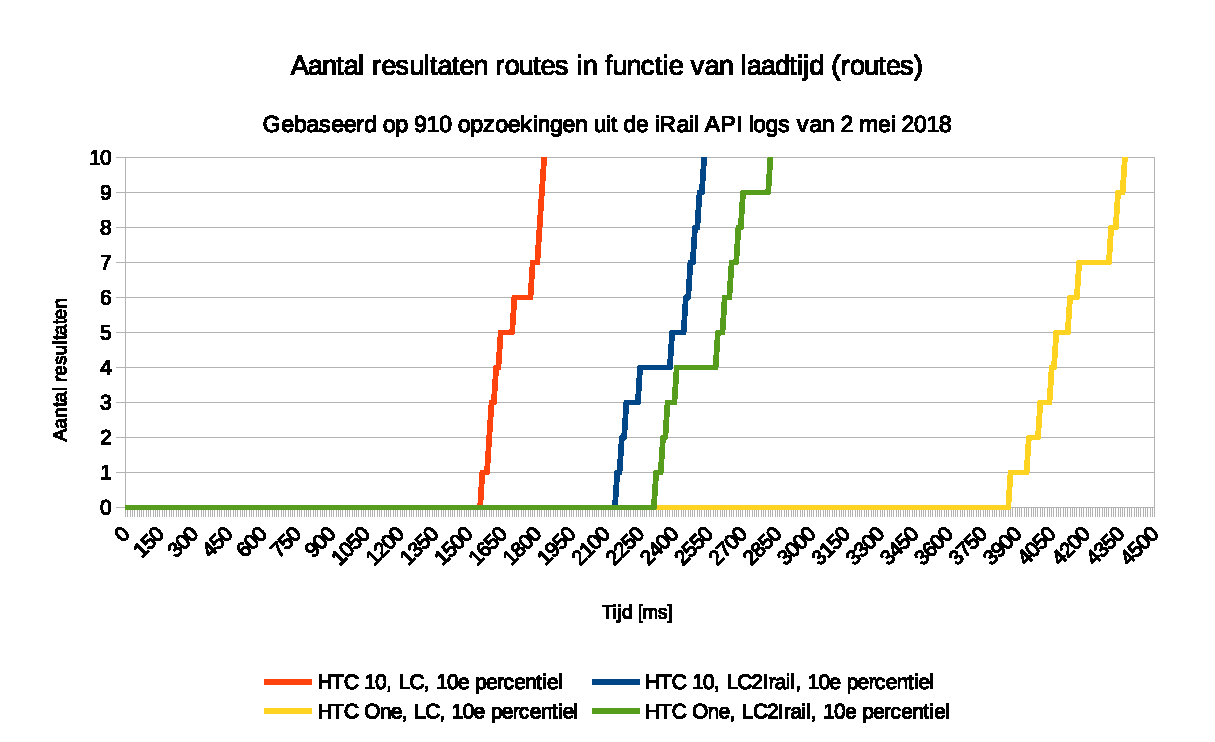
\includegraphics[width=1.00\textwidth]{dief_routes_best.eps}
	\caption[Aantal resultaten routes in functie van de tijd]{Het aantal resultaten in functie van de verlopen tijd.}
	\label{fig:routesDiefBest}
\end{figure}

\begin{figure}[h]
	\centering
	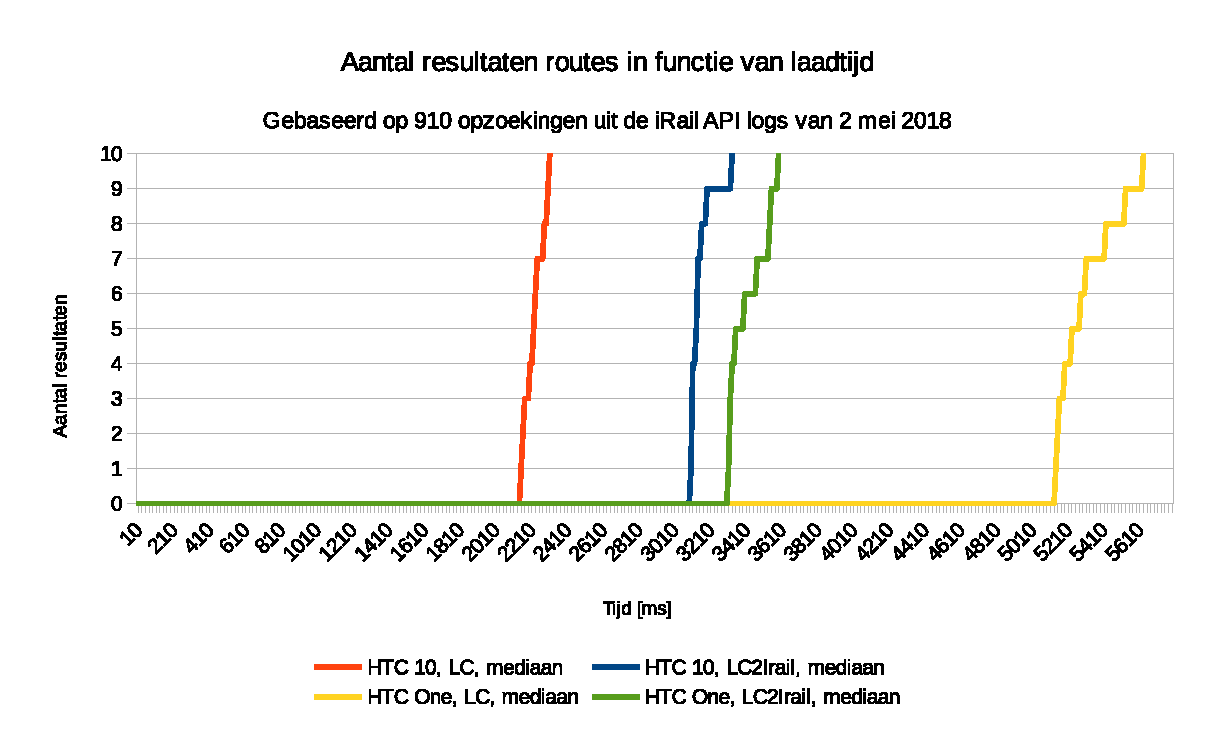
\includegraphics[width=1.00\textwidth]{dief_routes_gemiddeld.eps}
	\caption[Aantal resultaten routes in functie van de tijd]{Het aantal resultaten in functie van de verlopen tijd.}
	\label{fig:routesDiefAvg}
\end{figure}

\begin{figure}[h]
	\centering
	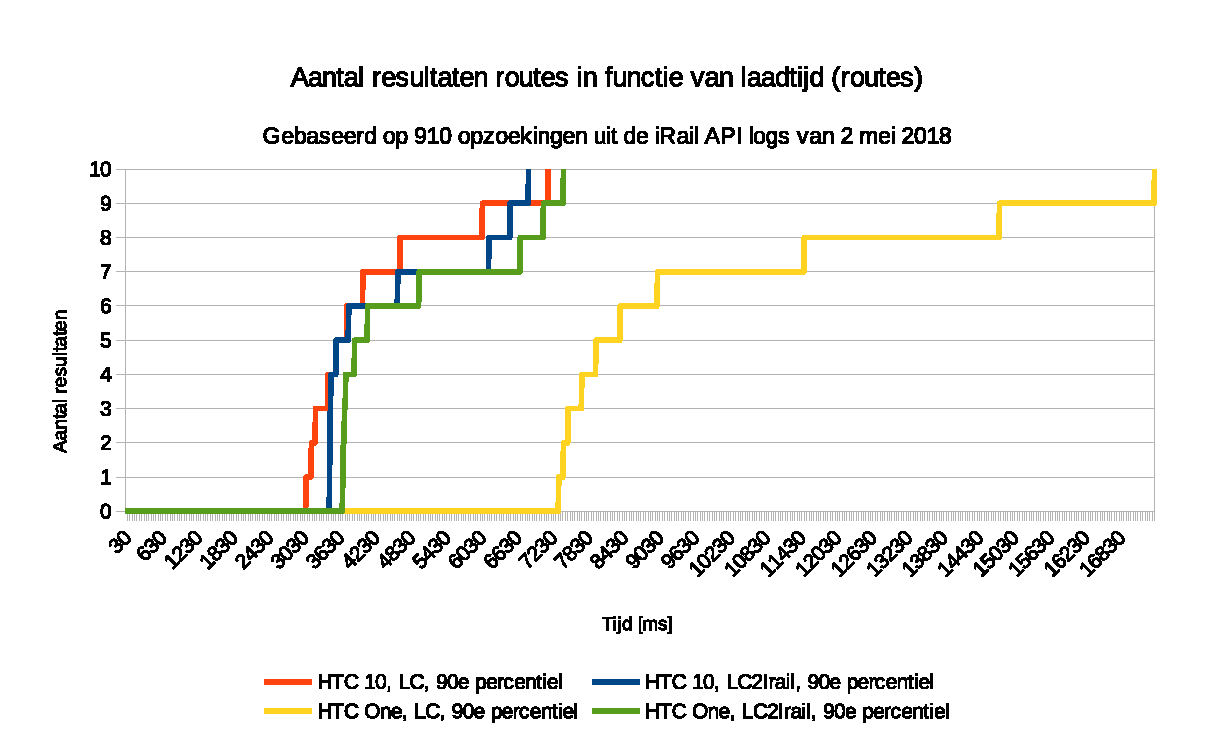
\includegraphics[width=1.00\textwidth]{dief_routes_slechtst.eps}
	\caption[Aantal resultaten routes in functie van de tijd]{Het aantal resultaten in functie van de verlopen tijd.}
	\label{fig:routesDiefSlechtst}
\end{figure}

Uit deze grafieken kunnen we opnieuw duidelijke conclusies trekken:
\begin{itemize}
	\item In alle grafieken en voor alle testen, hebben de curves een gelijkaardige vorm, waarbij er na een relatief lange wachttijd aan snel tempo resultaten geladen worden: in het geval van Linked Connections is voor de eerste opzoeking telkens een relatief grote hoeveelheid data nodig is, waarna slechts één of twee extra pagina's moeten opgehaald worden om het volgend resultaat te bepalen. In het geval van LC2Irail worden resultaten in grote blokken binnengehaald, waarbij vanaf de tweede opzoeking reeds veel data in cache zit. In het geval van LC2Irail worden resultaten ook onmiddellijk voor grote intervallen opgehaald, om zo het aantal verzoeken te beperken. 
	\item Terwijl op de HTC 10 Linked Connections in alle gevallen beter presteert dan LC2Irail, presteert Linked Connections slechter dan LC2Irail op de HTC One. 
	\item Opnieuw presteert LC2Irail op beide toestellen gelijkaardig, met slechts een kleine verschuiving in tijd tussen beide curves.
	\item Terwijl in het slechtste geval bijna alle varianten gelijk presteren, loopt Linked Connections op de HTC One enorm achter. Uit alle grafieken volgt dat hoe trager het toestel, hoe trager Linked Connections, terwijl LC2Irail ongeveer even goed blijft presteren. Bijgevolg kunnen we dus ook stellen, dat alle toestellen trager dan de HTC10 in het slechtste geval trager zullen presteren dan de HTC One.
	\item In alle gevallen laadt het eerste resultaat pas na anderhalve tot zeven seconden. Dit zijn zeer lange laadtijden, waarvan we verwachten dat ze de gebruikerservaring negatief gaan beïnvloeden.
\end{itemize}

Wanneer we nu specifiek naar de verdelingen kijken, gevisualiseerd door middel van de box plots in figuur~\ref{fig:routesBoxplot1} en~\ref{fig:routesBoxplot10}, zien we sterke verschillen, zowel tussen toestellen als implementaties. Net als bij liveboards zien we ook hier duidelijk hoe LC2Irail gelijke prestaties heeft op beide toestellen, met bijna identieke distributies. Dit in tegenstelling tot de prestaties van Linked Connections, die zeer sterk variëren per toestel. Op de HTC 10 zal voor al meer dan 75\% van de opzoekingen via Linked Connections het eerste resultaat geladen zijn op het moment dat LC2Irail op hetzelfde toestel minder dan 25\% van de verzoeken beantwoordt heeft. Op het HTC One toestel is dit echter omgekeerd, en nog extremer. 

Voor het tiende resultaat zijn deze verschillen tussen toestellen iets minder extreem, al zijn ze nog steeds zeer groot. Linked Connections blijft iets consistentere resultaten bieden op de HTC 10, terwijl de HTC One net minder consistente resultaten biedt dan LC2Irail. LC2Irail biedt ook voor het tiende resultaat exact dezelfde ervaring op beide toestellen, terwijl het verschil tussen de mediaan voor Linked Connections op beide toestellen niet acceptabel is en de gebruikerservaring duidelijk zal beïnvloeden.

\begin{figure}[h]
	\centering
	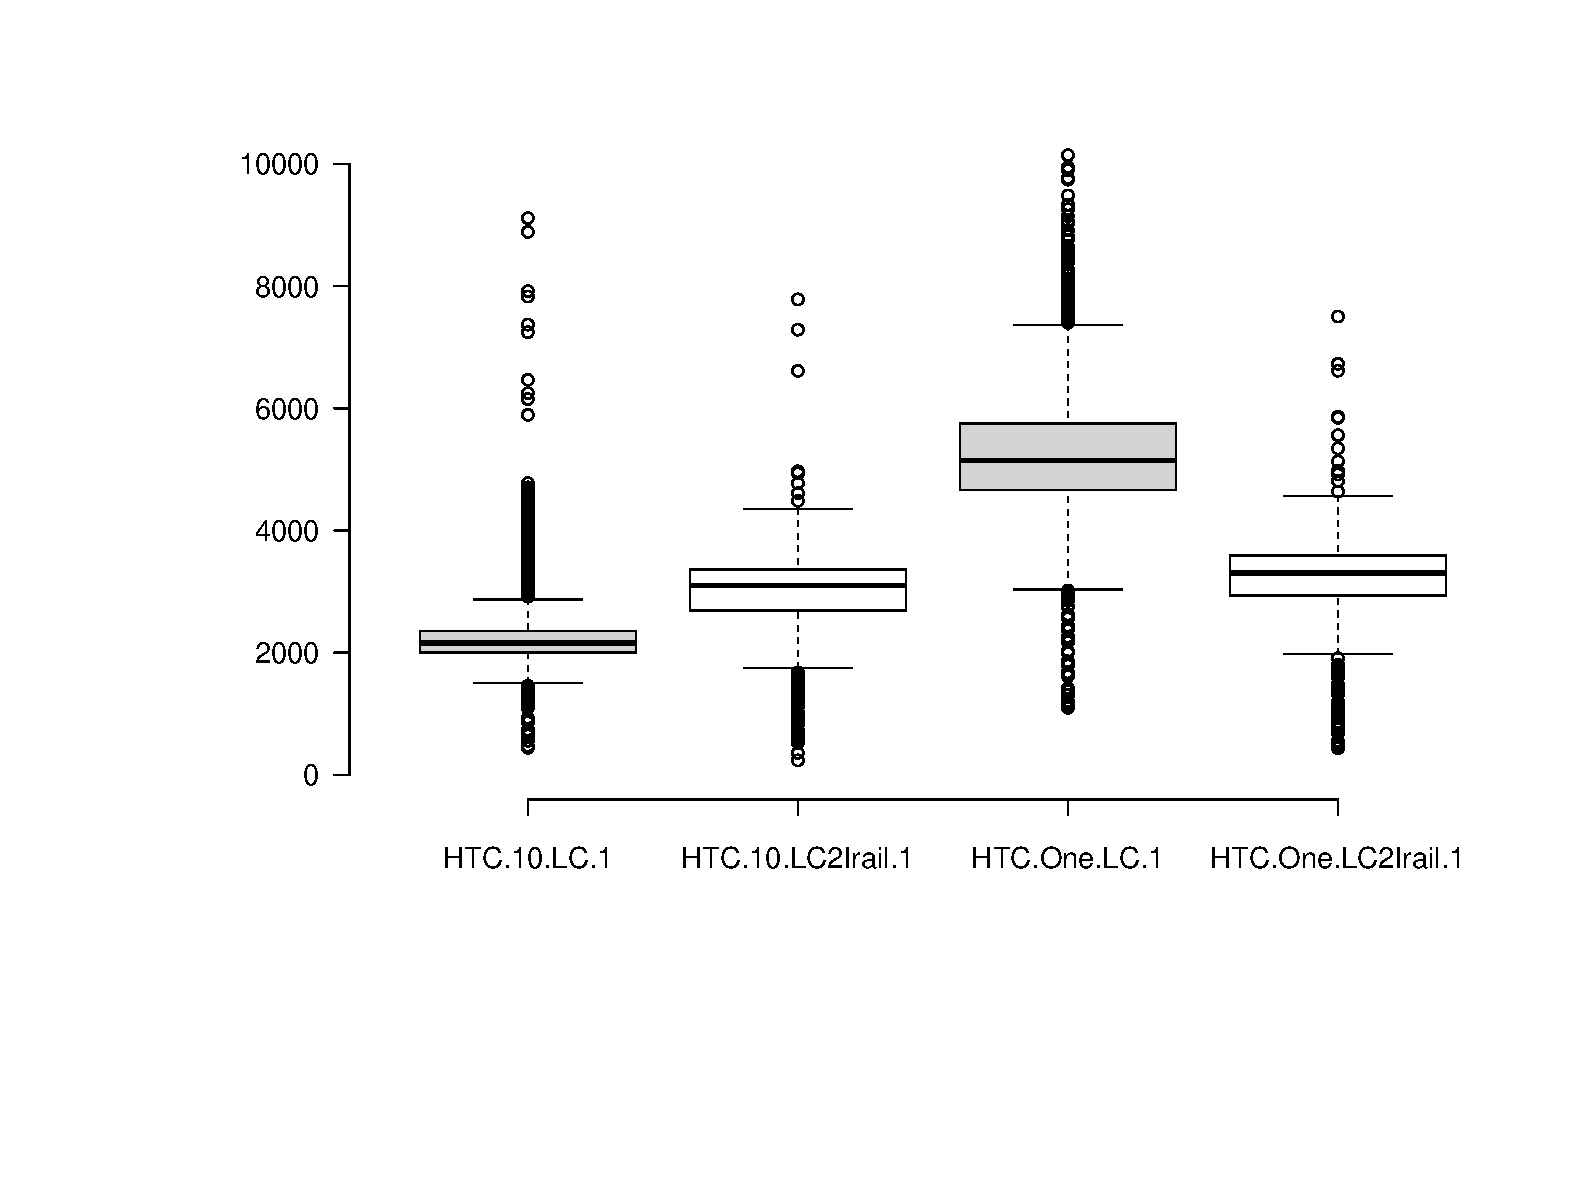
\includegraphics[width=0.80\textwidth]{boxplot_routes_1.eps}
	\caption[Laadtijd eerste resultaat route in functie van toestel en technologie]{Laadtijd eerste resultaat route in functie van toestel en technologie.}
	\label{fig:routesBoxplot1}
\end{figure}

\begin{figure}[h]
	\centering
	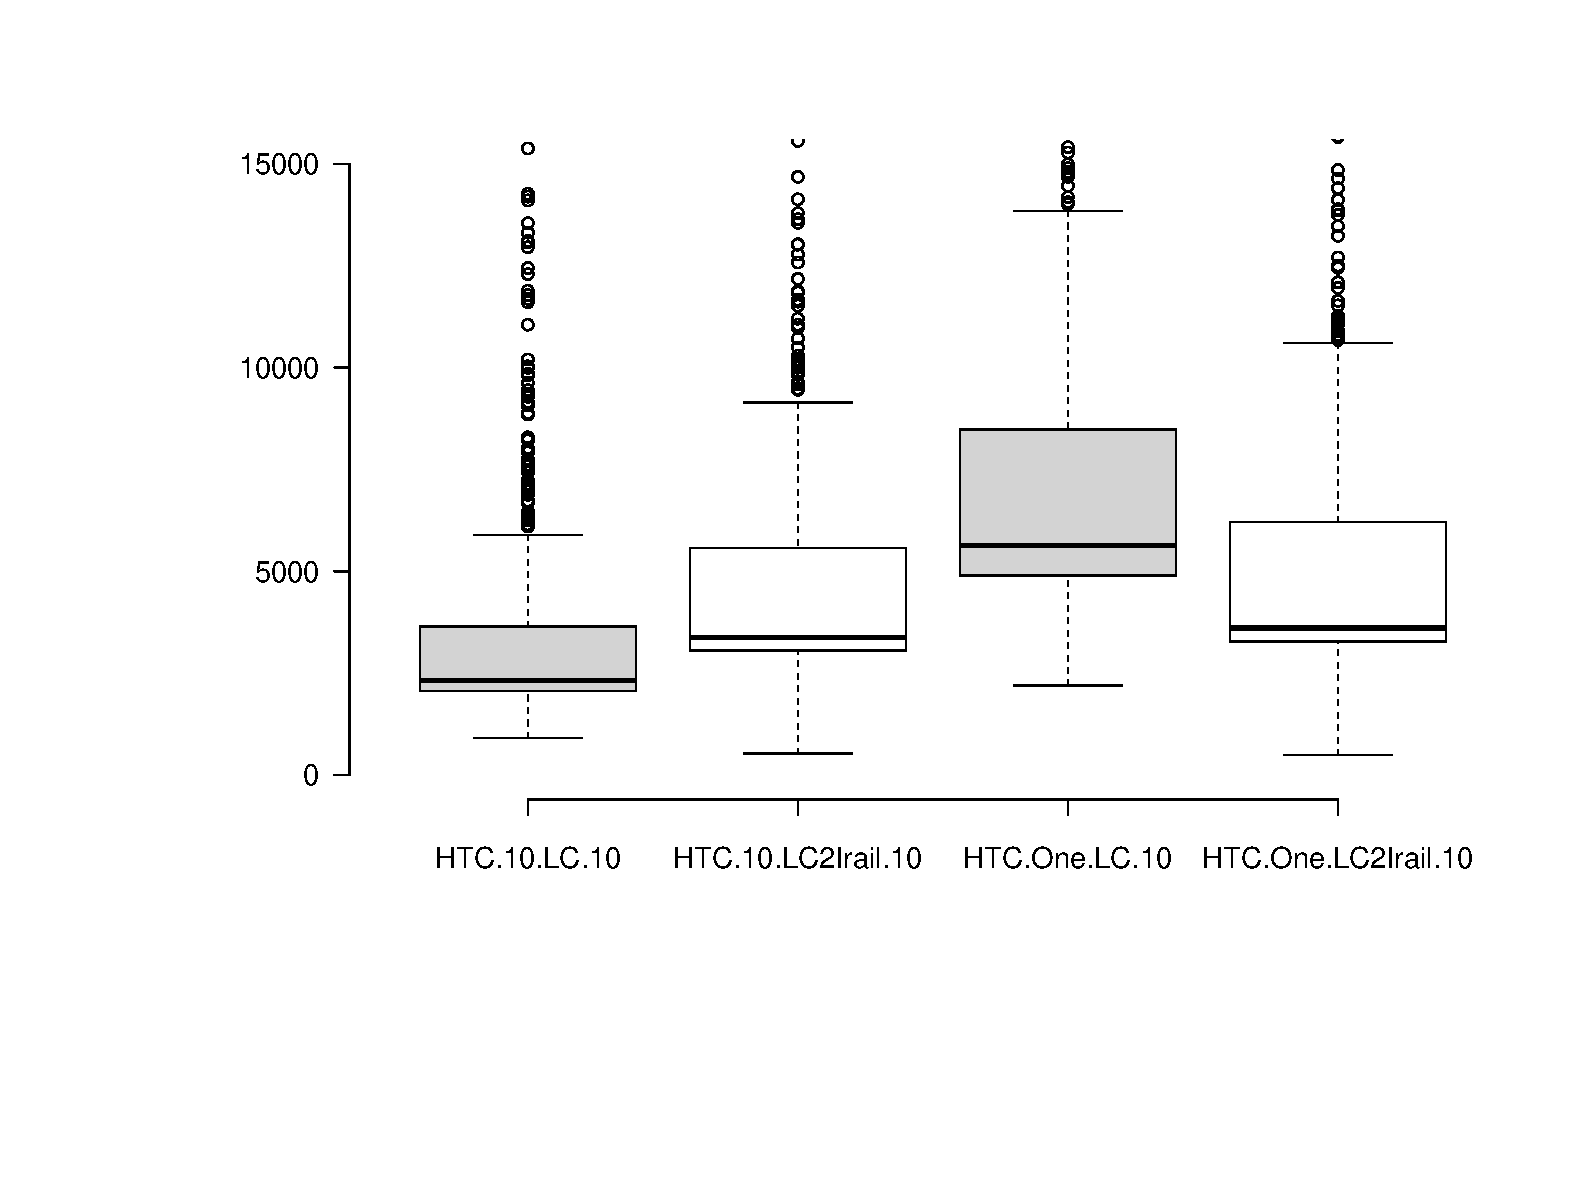
\includegraphics[width=0.80\textwidth]{boxplot_routes_10.eps}
	\caption[Laadtijd tiende resultaat route in functie van toestel en technologie]{Laadtijd tiende resultaat route in functie van toestel en technologie.}
	\label{fig:routesBoxplot10}
\end{figure}

\subsection{Ervaringen}

Op vlak van gebruikerservaring verwachten we dat gebruikers net zoals bij Liveboards de implementatie op basis van LC2Irail consistenter zullen beoordelen, en dat, afhankelijk van het door de tester gebruikte toestel, Linked Connections sneller, even snel of trager dan LC2Irail ervaren wordt.

\begin{figure}[h]
	\centering
	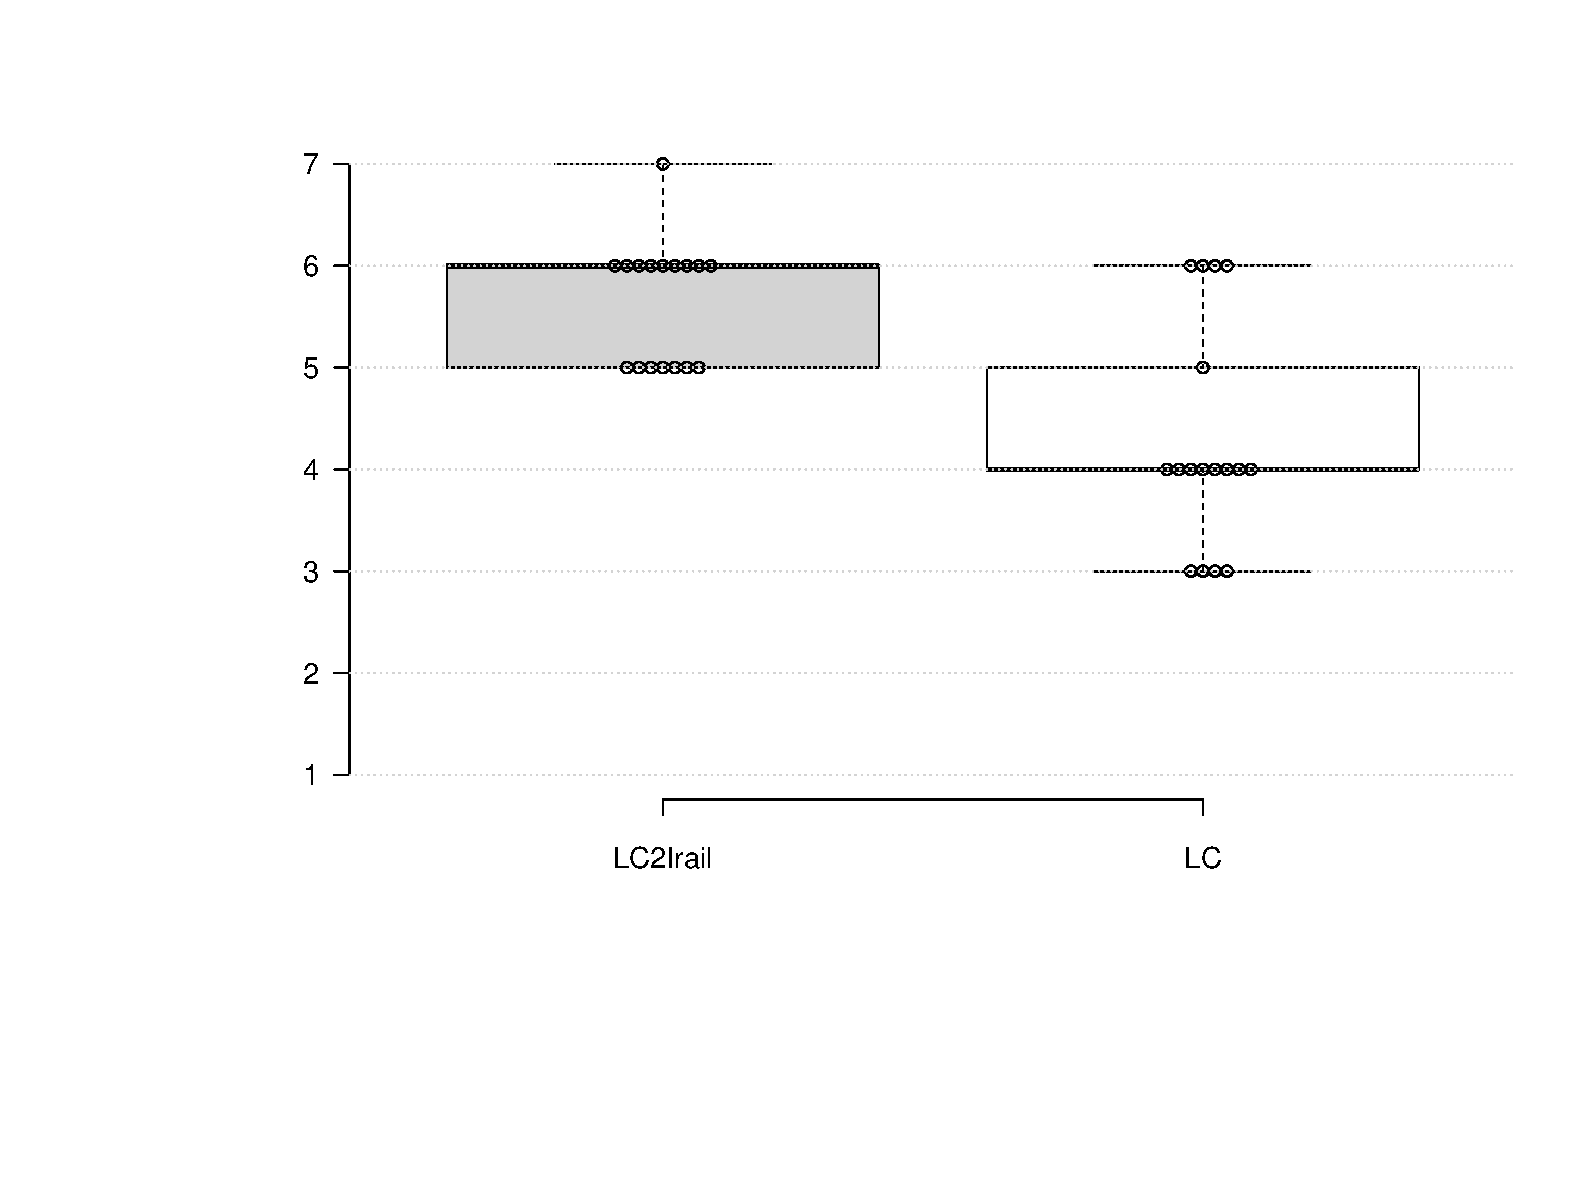
\includegraphics[width=0.80\textwidth]{boxplot_routes_ux.eps}
	\caption[Ervaren snelheid van routes]{De ervaren snelheid op een schaal 1-7 van routes voor LC2Irail en Linked Connections, gebaseerd op 17 user-tests.}
	\label{fig:routesUx}
\end{figure}

Wanneer we nu de resultaten van user-testing vergelijken met de verwachtingen, blijken deze verwachtingen grotendeels in vervulling te gaan. In figuur~\ref{fig:routesUx} is te zien dat de prestaties van LC2Irail iets consistenter goed beoordeeld worden, en LC2Irail een betere beoordeling krijgt dan Linked Connections. In vergelijking met liveboards (figuur~\ref{fig:liveboardsUx}) zien we dat gebruikers bij routes iets minder verdeeld zijn over de prestaties van Linked Connections, al komt dit omdat er geen gebruikers voor de hoogste score kiezen. 

De consistentere beoordelingen voor Linked Connections zijn ook duidelijk wanneer we dieper ingaan op hoe eenzelfde gebruiker de snelheid van LC2Irail en Linked Connections ervaart, zichtbaar in figuur~\ref{fig:alluvialUserChoicesRoutes}. Hoewel veel gebruikers Linked Connections als trager ervaren, is er ook een klein aantal gebruikers dat Linked Connections sneller ervaart. Het zijn deze personen die, wanneer expliciet gevraagd wordt om de snelste implementatie aan te duiden, voor Linked Connections kiezen. Dit duidelijk verband kon bij liveboards niet gelegd worden (figuur~\ref{fig:alluvialUserChoicesLiveboards}), wat te wijten kan zijn aan een voor gebruikers slechts een klein, onduidelijk verschil was tussen de prestaties bij liveboards. Voor routes wordt het verschil veel duidelijker ervaren, en kiezen gebruikers dus consistenter met de door hun ervaren snelheden.

Opvallend is ook dat er een persoon is die Linked Connections als zeer snel bestempelt, en Linked Connections hiermee even snel of sneller dan LC2Irail ervaart. Echter kiest deze persoon toch voor LC2Irail wanneer een expliciete keuze gemaakt dient te worden. We kunnen stellen dat voor deze gebruiker het verschil niet merkbaar was. Aan de andere kant kiest iedereen die Linked Connections als traag of gemiddeld ervaart voor LC2Irail, op één gebruiker na die onbeslist is. Voor deze gebruikers moet Linked Connections nog sneller gemaakt worden alvorens het concurrentieel wordt.

\begin{figure}[ht]
	\centering
	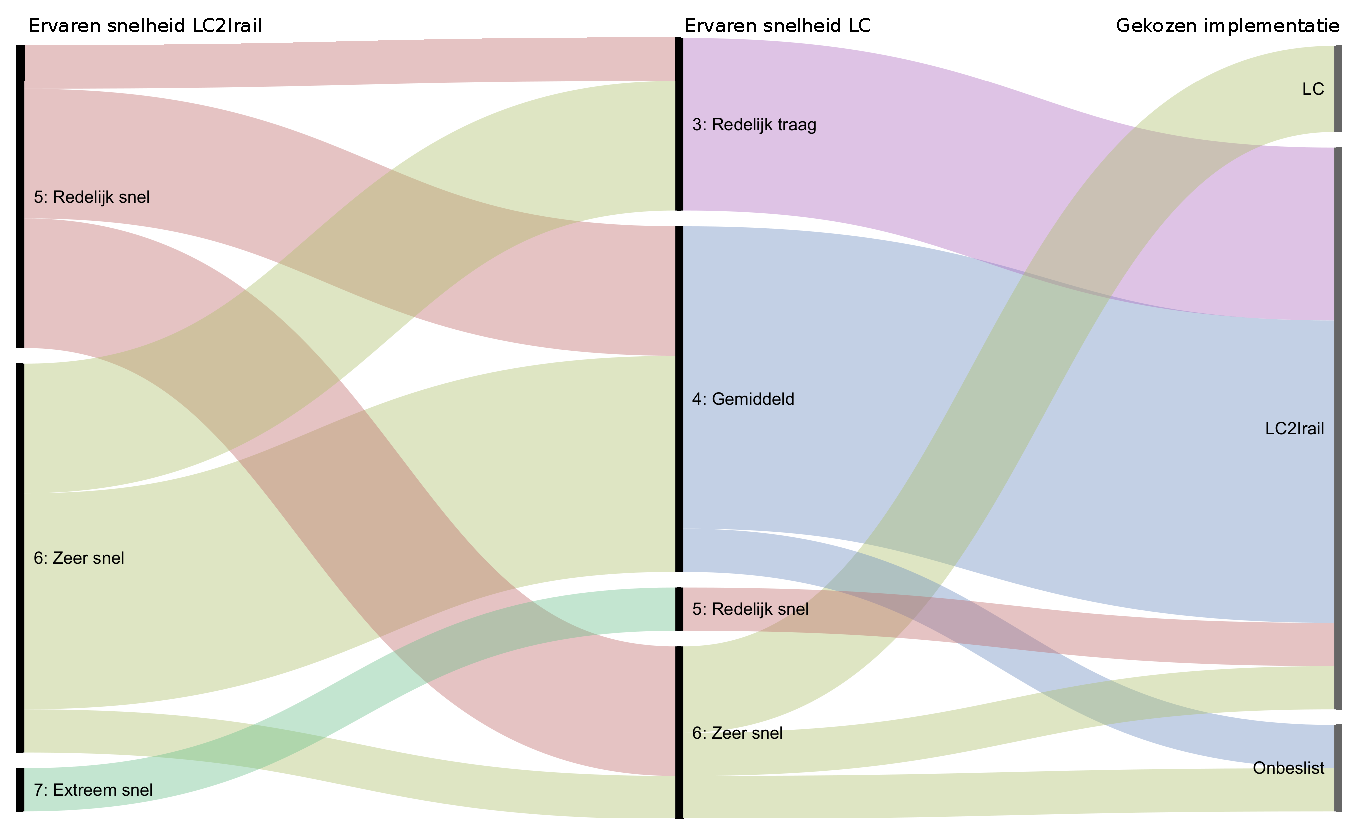
\includegraphics[width=1.00\textwidth]{alluvial_user_choice_routes.eps}
	\caption[Door gebruikers gekozen implementatie voor routes]{Verbanden tussen de door gebruikers gekozen implementaties voor routes. }
	\label{fig:alluvialUserChoicesRoutes}
\end{figure}

Wanneer we voor routes beide JSON parsers vergelijken, zien we dat voor de \foreign{LoganSquare} parser de proefpersonen een meer uitgesproken mening hadden: er waren zowel meer tevreden als ontevreden personen, terwijl bij de \foreign{org.json} parser veel mensen neutraal waren. Dit gaat echter in tegen een praktijktest waarbij enkele gebruikers achtereenvolgens een versie gebruikmakend van de \foreign{org.json} en \foreign{LoganSquare} parser voorgeschoteld kregen, gaven deze telkens aan de versie op basis van \foreign{LoganSquare} sneller te ervaren, zowel op goedkope als dure smartphones. Hieruit besluiten we dat de gebruikerstests, opgedeeld per parser, te kleine steekproeven zijn om een algemene conclusie te vormen over de invloed van de parsers.

\begin{figure}[ht]
	\centering
	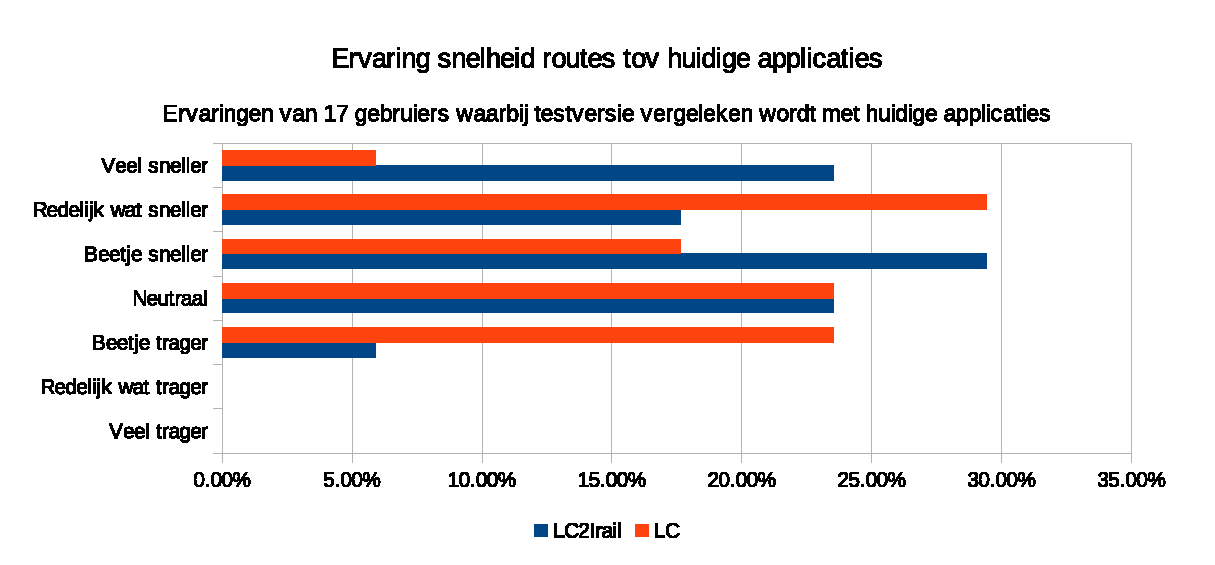
\includegraphics[width=1.00\textwidth]{userdata_routes_currentapp.eps}
	\caption[Door gebruikers ervaren snelheid routes tov huidige apps]{De door 17 gebruikers ervaren snelheid routes ten opzichte huidige apps }
	\label{fig:relativePerceptionRoutes}
\end{figure}

Als tot slot gevraagd wordt om de snelheid te vergelijken met de applicatie die de gebruiker op dit moment gebruikt, doen beide testversies het goed ten opzichte van de huidige applicaties. Dit is zichtbaar in figuur~\ref{fig:relativePerceptionRoutes}. Linked Connections scoort iets minder goed dan LC2Irail, maar de overgrote meerderheid vindt Linked Connections nog steeds even snel of sneller dan de applicatie die men gewoonlijk gebruikt.

\section{Voertuigen}

\subsection{Metingen}
Het opzoeken van het traject dat een voertuig aflegt verschilt sterk van de eerder besproken endpoints. Het traject van een voertuig wordt door HyperRail als één (ondeelbaar) resultaat beschouwd, en kan hierdoor niet per stop geladen worden. Dit in tegenstelling tot liveboards en routes, waar er verschillende resultaten zijn die elk onafhankelijk van elkaar zijn.

Dit is ook de opzoeking die het meeste data vereist bij Linked Connections: alle pagina's moeten doorzocht worden op connecties met betrekking tot één specifiek voertuig. Dit voertuig komt slechts in een relatief beperkt aantal pagina's voor, gezien het voertuig slechts enkele uren rijdt, en het tijdstip van vertrek en aankomst onbekend zijn. Zoals eerder vermeld %TODO: referntie %TODO: aantal stops
zijn hier enkele oplossingen voor, zoals het gebruik van een index. We definiëren een index in deze context als een lijst van alle treinen voor een bepaalde periode (in dit geval mei 2018) en het tijdstip van hun eerste vertrek.

Om een idee te krijgen van de invloed van deze index, alsook van het gebruik van een cachegeheugen voor de Linked Connections pagina's bij deze opzoekingen, werden 102 voertuigen opgezocht, voor alle combinaties van cache en index gebruik. Tevens werd een extra test gedaan met een cache die in het RAM geheugen geplaatst wordt (in tegenstelling tot het flashgeheugen van het toestel), en een vergelijkende test waarbij de Linked Connections server gebruikt werd. De gemiddelde opzoektijd hiervoor is gevisualiseerd in figuur~\ref{fig:vehiclelabtest}.

\begin{figure}[h]
	\centering
	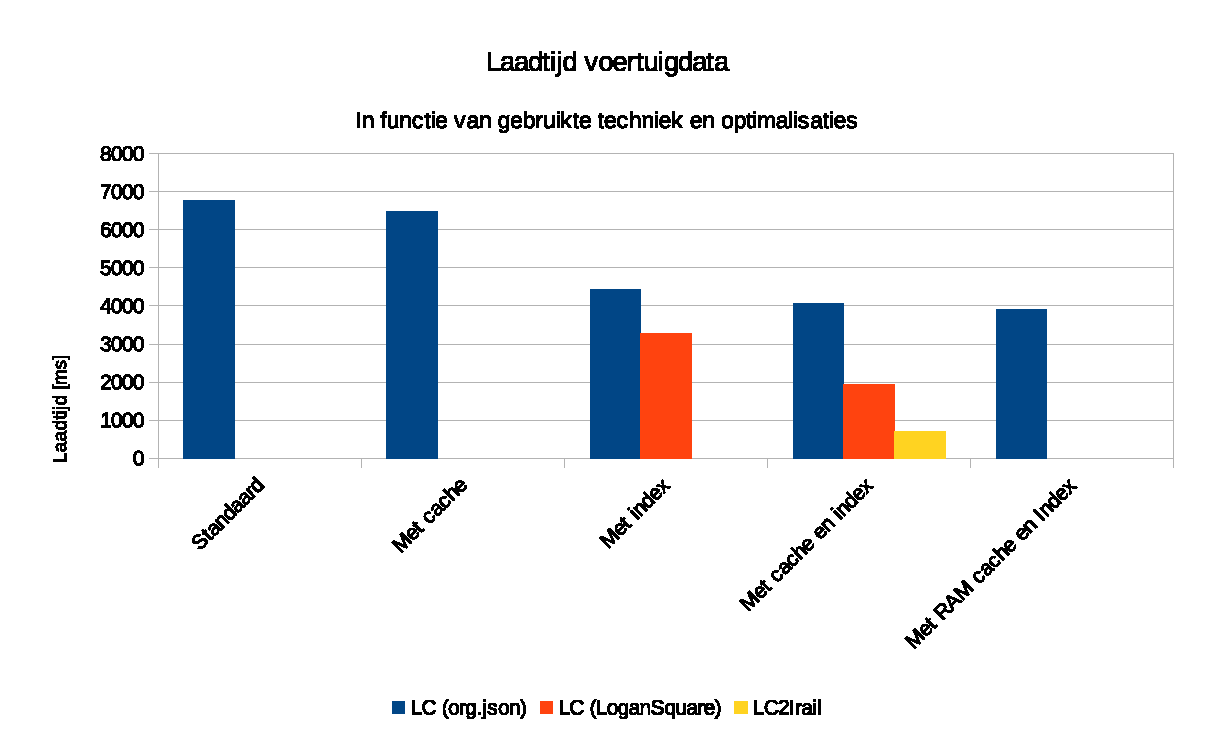
\includegraphics[width=1.00\textwidth]{Optimalisaties_voertuigen.eps}
	\caption[Gemeten laadtijd voertuigen]{De gemeten laadtijd voor voertuigen gebruikmakend van een HTC 10 voor 102 opzoekingen gebaseerd op de iRail logs. }
	\label{fig:vehiclelabtest}
\end{figure}

%\begin{table}[ht]
%	\begin{tabular}{| c | c | c | c | c | c | c |}
%		\hline
%		Variant & parser & cache & index & minimaal (ms) & gemiddelde (ms) & maximaal (ms)\\
%		\hline
%		LC op toestel & org.json & nee & nee & 540 & 6764 & 12676 \\
%		LC op toestel & org.json & ja & nee & 483 & 6488 & 10921 \\
%		
%		LC op toestel & org.json & nee & ja & 2638 & 4443 & 10956 \\
%		LC op toestel & org.json & ja & ja &  2440 & 4066 & 6003\\
%		LC op toestel & org.json & RAM & ja & 2263 & 3912 & 5763 \\
%		LC op toestel & LoganSquare & nee & ja &  1860 & 3283 & 5374 \\
%		LC op toestel & LoganSquare & ja  & ja & 1195 & 1925 & 2888 \\
%		
%		LC op server &&&&  264 & 713 & 5068 \\
%		\hline
%	\end{tabular}
%	\caption[Gemeten laadtijd voertuigen]{De gemeten laadtijd voor voertuigen gebruikmakend van een HTC 10 voor 102 opzoekingen gebaseerd op de iRail logs. }
%	\label{tab:vehiclelabtest}
%\end{table}

Het is duidelijk dat de standaard implementatie zeer slecht presteert. Ook het gebruik van een cachegeheugen brengt hierbij niet veel beterschap. Wanneer echter een index toegevoegd worden, is een drastische verbetering merkbaar. Het gemiddelde daalt in deze beperkte test met ongeveer een derde. Toevoeging van een cachegeheugen, op flash of in het RAM geheugen, brengt ook hier relatief weinig beterschap. 

Een tweede grote verbetering kan behaald worden door het gebruik van de eerder besproken \foreign{LoganSquare} parser. Hierbij zien we ook een veel grotere verbetering door cachegebruik dan bij de \foreign{org.json} parser. Dit is logisch, gezien bij het gebruik van de \foreign{LoganSquare} parser het verwerken van de data relatief gezien minder tijd in beslag neemt - het ophalen van data wordt dus belangrijker. Op het eerste zicht blijven alle lokale varianten veel trager dan de serverimplementatie, die sneller door pagina's kan zoeken.

We onderzoeken nu het verschil tussen de lokale implementatie en de serverimplementatie in detail. Hiervoor zoeken we 2102 ritten op die plaatsvinden op 6 mei 2018. Dit wordt enerzijds gedaan voor Linked Connections dat gebruik maakt van de \foreign{LoganSquare} parser, cache en lokale index, en anderzijds voor de serverimplementatie, die server-side over dezelfde index en een cache beschikt.

Wanneer we kijken naar de box-plot van de responstijd, weergegeven in figuur~\ref{fig:vehicleboxplot}, zien we dat de Linked Connections duidelijk slechter presteert. Op beide toestellen is LC2Irail sneller. Bij de HTC 10, valt dit nog enigszins mee, maar op de HTC One zijn via LC2Irail de meeste resultaten binnen 3000 milliseconden geladen, terwijl op dat moment nog geen 25\% van de opzoekingen via Linked Connections uitgevoerd werd. Net zoals bij liveboards en routes zien we hier dat LC2Irail consistente prestaties biedt: beide box plots zijn ongeveer identiek, op wat uitlopers na. Voor Linked Connections zien we echter dat, net zoals voor het opzoeken van liveboards en routes, de spreiding van de benodigde tijd afhangt van het toestel: een traag toestel zal niet alleen trager resultaten laden, maar heeft ook een grotere variatie in de laadtijd.

\begin{figure}[h]
	\centering
	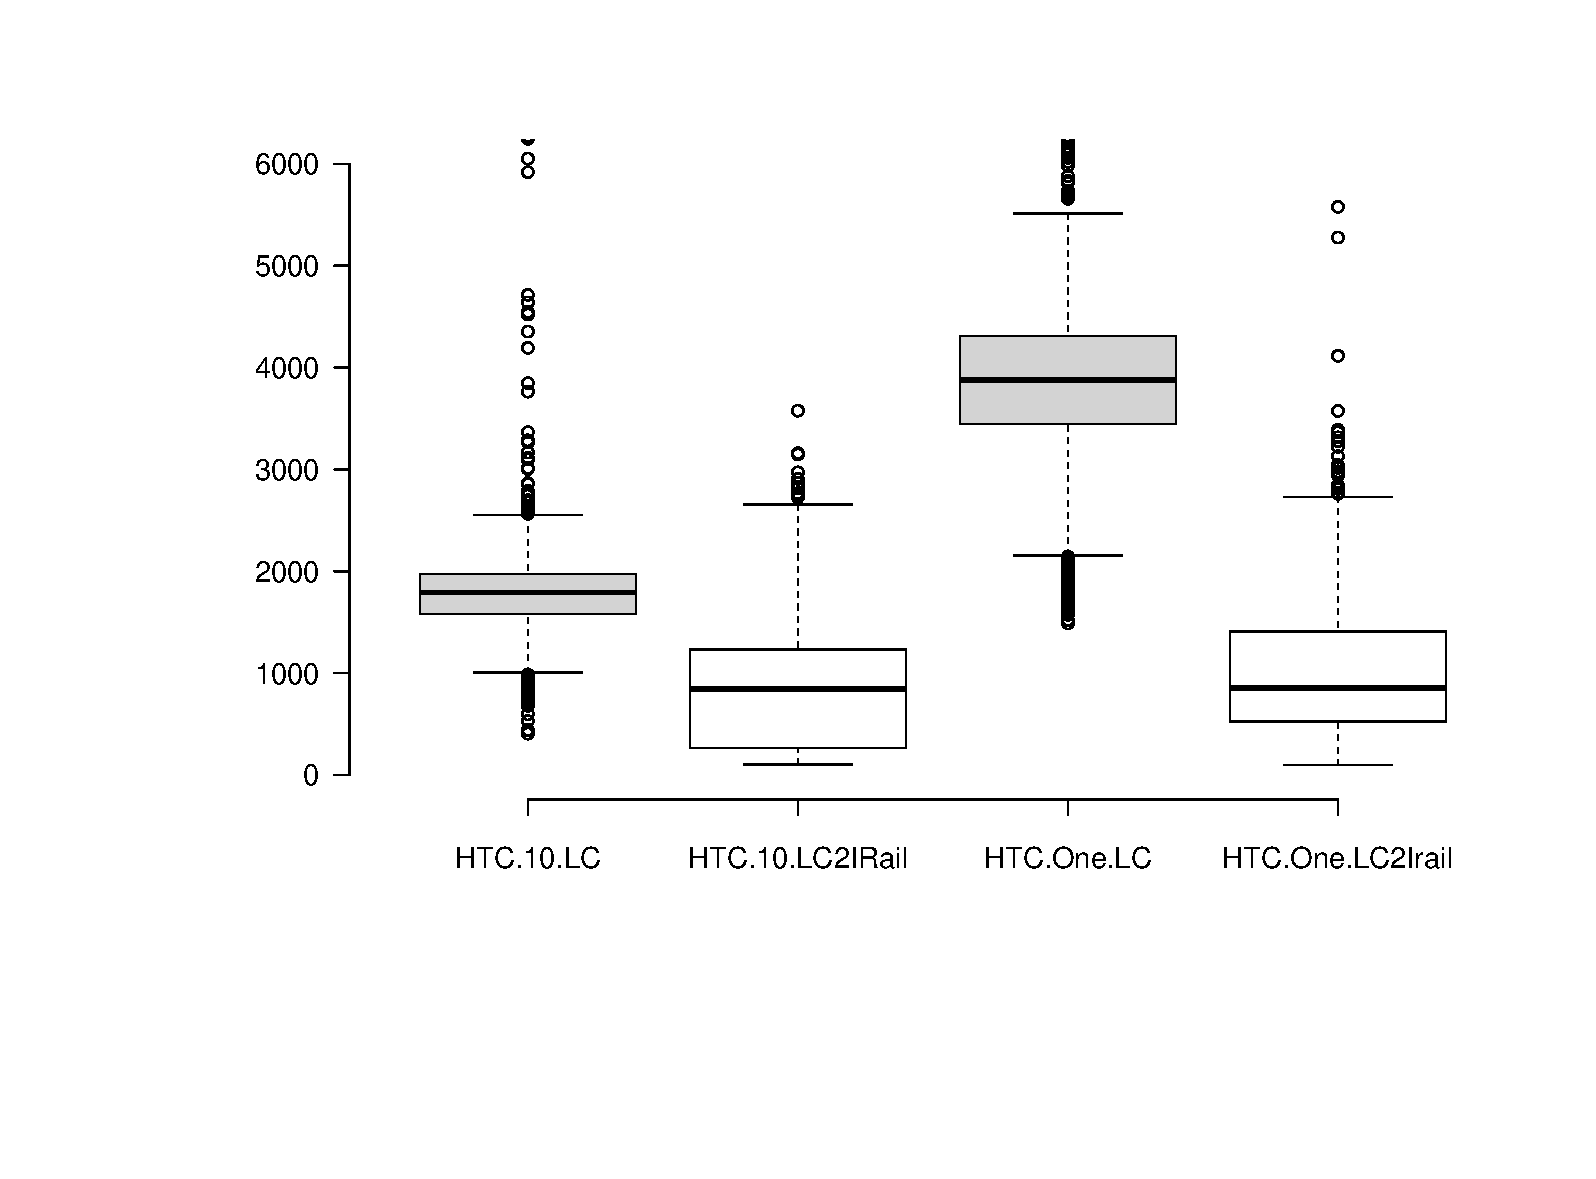
\includegraphics[width=1.00\textwidth]{boxplot_vehicles.eps}
	\caption[Prestaties voor het laden van voertuigen]{De prestaties voor het laden van voertuigen, gemeten door alle voertuigen, beschreven in Linked Connections, voor 6 mei op te zoeken.}
	\label{fig:vehicleboxplot}
\end{figure}

%\begin{figure}[h]
%	\centering
%	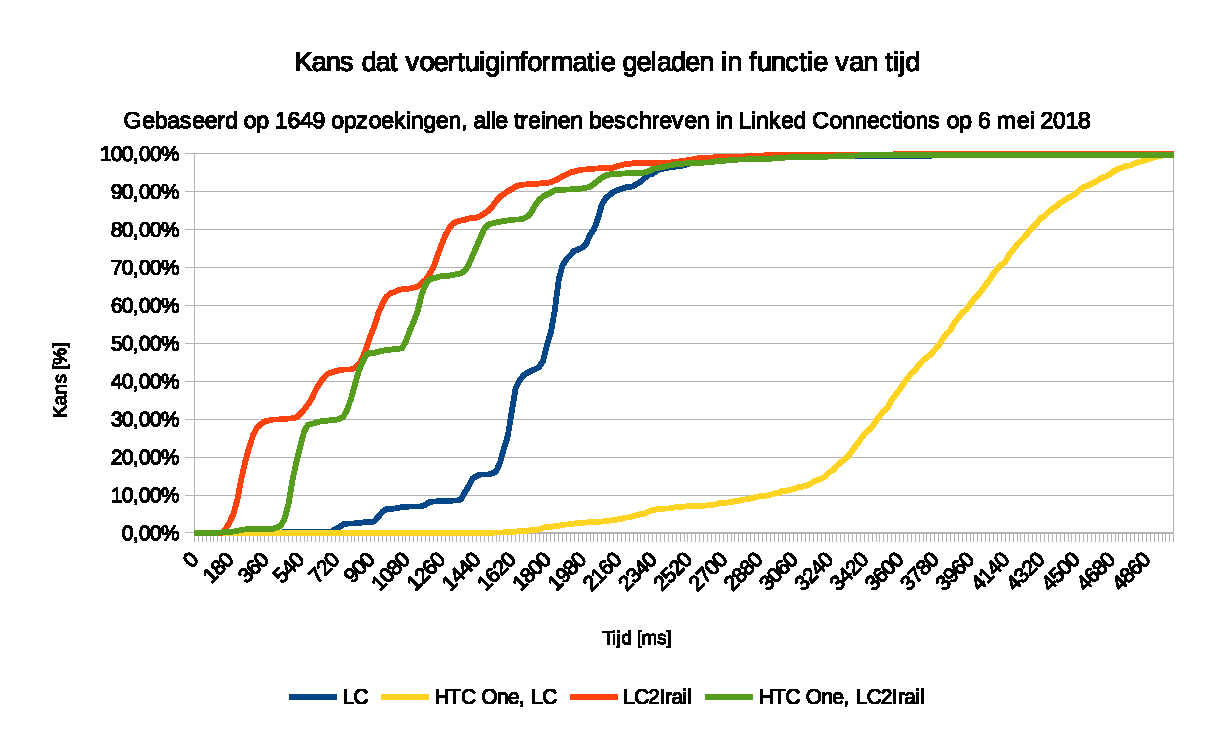
\includegraphics[width=1.00\textwidth]{distribution_vehicle_loading_cummulatief.eps}
%	\caption[Cummulatieve kans op laden van voertuig]{De kans dat een voertuig geladen is in functie van de verlopen tijd.}
%	\label{fig:vehiclecummulatief}
%\end{figure}

\subsection{Ervaringen}
Wanneer we nu de resultaten van de user-testing bekijken, zien we zoals verwacht dat het laden van voertuigen beduidend slechter scoort wanneer de lokale Linked Connections implementatie gebruikt wordt, vergeleken met wanneer de serverimplementatie gebruikt werd. In figuur~\ref{fig:vehicleboxplot} is dit duidelijk zichtbaar. Zo beoordelen de meeste gebruikers Linked connections slechts als "gemiddeld", terwijl de meerderheid van de gebruikers de LC2Irail variant als "Zeer snel" bestempelde. Ook zien we hier, net als bij liveboards en routes, dat er voor Linked Connections een veel grotere spreiding is in de gegeven antwoorden, terwijl bij LC2Irail iedereen het er over eens lijkt dat deze implementatie snel is.

\begin{figure}[h]
	\centering
	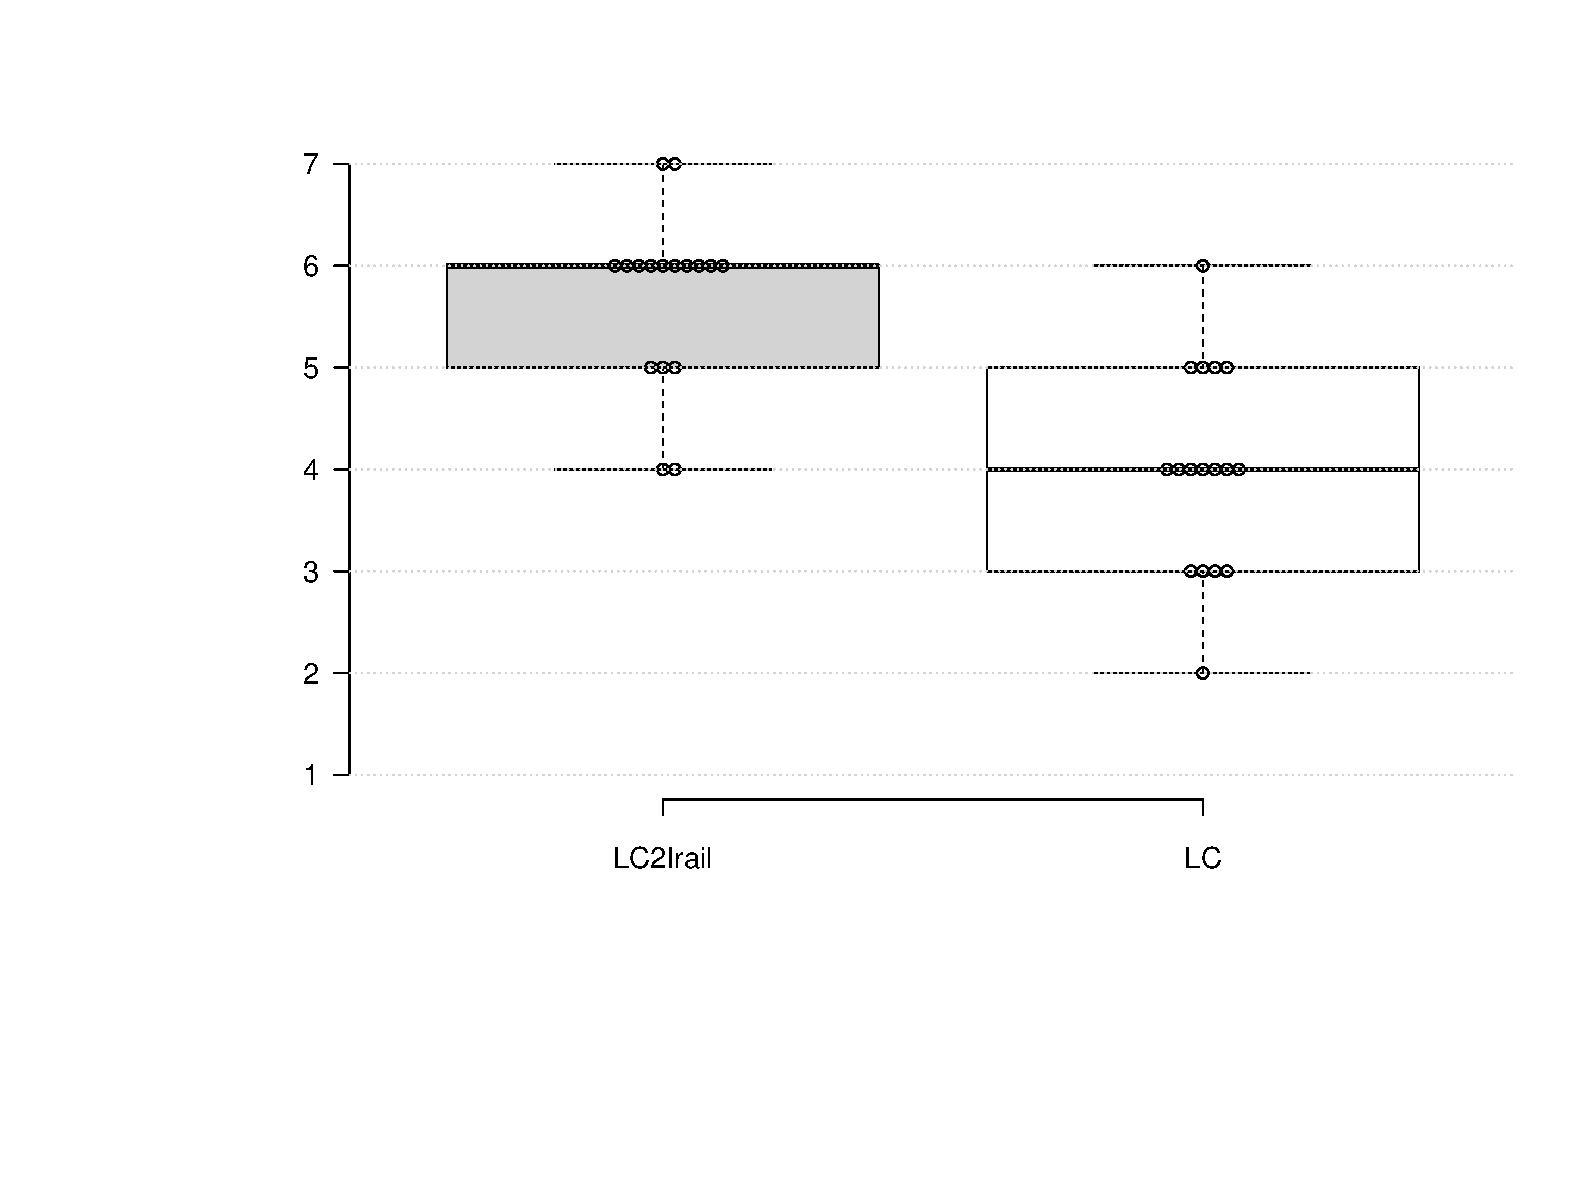
\includegraphics[width=1.00\textwidth]{boxplot_vehicles_ux.eps}
	\caption[Ervaren snelheid van routes]{De ervaren snelheid op een schaal 1-7 van routes voor LC2Irail en Linked Connections, gebaseerd op 17 user-tests.}
	\label{fig:vehiclesUx}
\end{figure}

Wanneer we de testgroep van Linked Connections opsplitsen per gebruikte parser, blijkt dat personen die de lokale implementatie op basis van \foreign{LoganSquare} testten, de laadtijd iets beter beoordeelden vergeleken met de groep die de implementatie op basis van de \foreign{org.json} parser testte. Deze resultaten liggen ook in lijn met ervaringen van testers die beide parsers achtereenvolgens voorgeschoteld kregen, waarbij alle testers de \foreign{LoganSqare} parser sneller ervoeren. Ondanks dat de testgroep onvoldoende groot was om een veralgemening te kunnen maken, kunnen we in combinatie met de directe vergelijking wel stellen dat er een grote kans is dat verbeteringen in de implementatie de snelheid verder omlaag kunnen brengen, en zo de gebruikerservaring kunnen verbeteren. Gezien bij het berekenen van voertuigen het meeste data nodig is, is hier de impact van implementatiedetails het grootst.

\begin{figure}[ht]
	\centering
	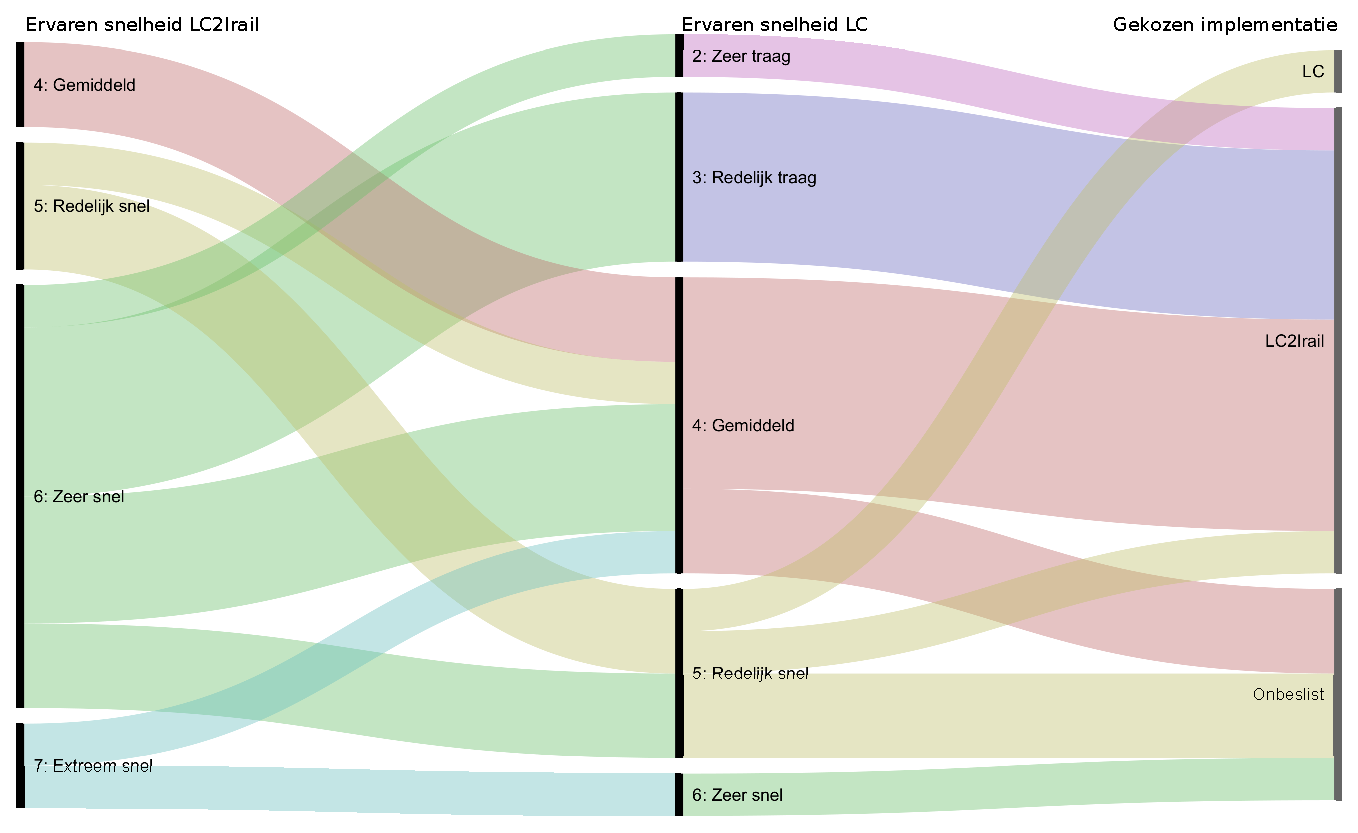
\includegraphics[width=1.00\textwidth]{alluvial_user_choice_vehicles.eps}
	\caption[Door gebruikers gekozen implementatie voor voertuigen]{Verbanden tussen de door gebruikers gekozen implementaties voor voertuigen. }
	\label{fig:alluvialUserChoicesVehicles}
\end{figure}

Wanneer de gebruiker gevraagd werd te kiezen, koos slechts één gebruiker voor de lokale implementatie in dit onderdeel. Vijf gebruikers hadden geen specifieke voorkeur voor een specifieke implementatie, ook al beoordeelden vier van hen Linked Connections als trager. In figuur~\ref{fig:alluvialUserChoicesVehicles} zijn de ervaringen van elke gebruiker duidelijk te zien. Zo zien we dat de ervaring voor gebruikers nooit verbeterd, en veel gebruikers een groot verschil ervaren tussen de snelheid van beide implementaties, in het nadeel van Linked Connections. Veel gebruikers die Linked Connections als redelijk of zeer snel ervaren, ervoeren LC2Irail nog steeds als sneller, waardoor ze wanneer ze moesten kiezen niet voor Linked Connections kozen. De enigste gebruiker die voor Linked Connections koos, ervoer Linked Connections niet als sneller dan LC2Irail, maar vond beide wel snel.

\begin{figure}[ht]
	\centering
	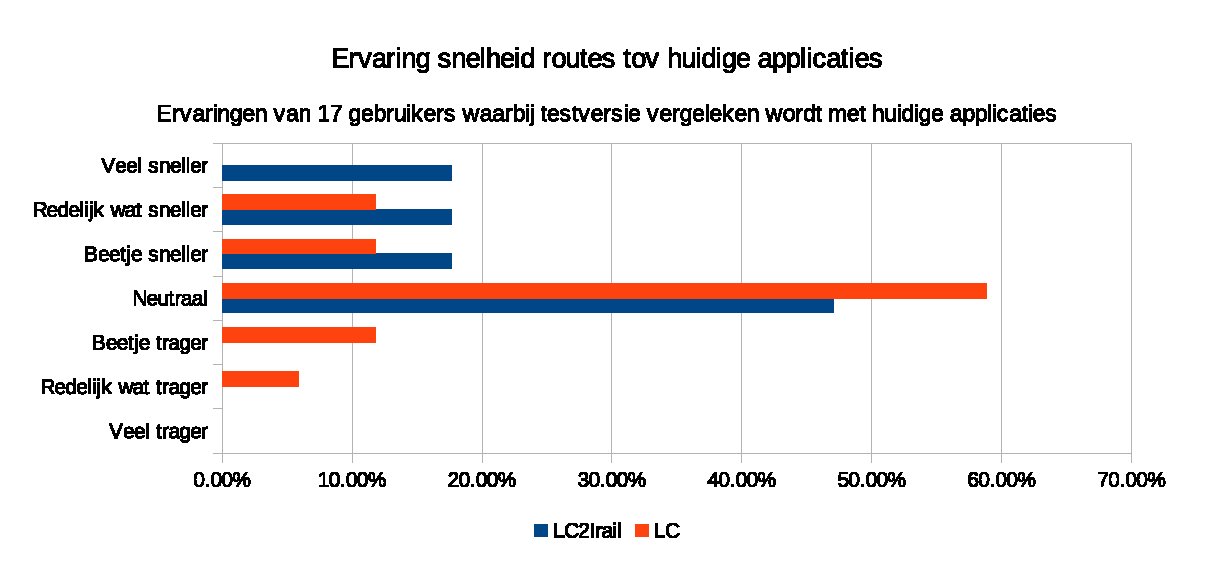
\includegraphics[width=1.00\textwidth]{userdata_vehicles_currentapp.eps}
	\caption[Door gebruikers ervaren snelheid voertuigen tov huidige apps]{De door 17 gebruikers ervaren snelheid routes ten opzichte huidige apps }
	\label{fig:relativePerceptionVehicles}
\end{figure}

Als gevraagd wordt om de snelheid te vergelijken met de applicatie die de gebruiker op dit moment gebruikt, geven zes op tien gebruikers aan Linked Connections als even snel te ervaren als hun huidige applicatie voor het opzoeken van voertuigen. De andere gebruikers geven aan de opzoekingen redelijk wat trager tot redelijk wat sneller te ervaren. Dit is duidelijk zichtbaar in figuur~\ref{fig:relativePerceptionVehicles}. Terwijl LC2Irail acceptabel scoort, blijkt Linked Connections hier toch achterop te raken, zowel ten opzichte van LC2Irail als ten opzichte van de Linked Connections prestaties voor voertuigen (figuur~\ref{fig:relativePerceptionLiveboards}) en routes (figuur~\ref{fig:relativePerceptionRoutes}).

\section{Door de gebruiker gekozen implementatie}

Voor alle soorten informatie (liveboards, routes, en voertuigen) lijkt Linked Connections een gelijkaardige of slechtere gebruikerservaring op te leveren dan LC2Irail in termen van laadtijd. Hierbij dienen we op te merken dat dit verschil bij liveboards slechts zeer beperkt is, en het laden nog steeds als snel werd ervaren. Voor routes bestempelden enkele personen Linked Connections als traag, maar ook hier blijft het verschil beperkt. Bij voertuigen blijkt echter dat Linked Connections door drie kwart van de gebruikers als trager werd ervaren, waarbij Linked Connections niet enkel relatief slechter scoort, maar ook in absolute termen slechts door een minderheid van de gebruikers als snel wordt ervaren. 

Linked Connections verschilt echter niet enkel in termen van laadtijd. Zoals eerder aangehaald in hypothese 1 is offline opzoeken mogelijk, en vermoeden we dat dit de keuze van de gebruiker beïnvloed. Om dit na te gaan hebben we de keuzes van gebruikers gevisualiseerd in figuur~\ref{fig:alluvialUserChoices}. In dit diagram zien we zowel hoeveel gebruikers voor elke implementatie kozen, maar ook hoe de keuze van gebruiker evolueert. Zo zien we dat naarmate de relatieve prestaties van LC ten opzichte van LC2Irail dalen, personen die eerder voor Linked Connections kozen overstappen op LC2Irail.

\begin{figure}[ht]
	\centering
	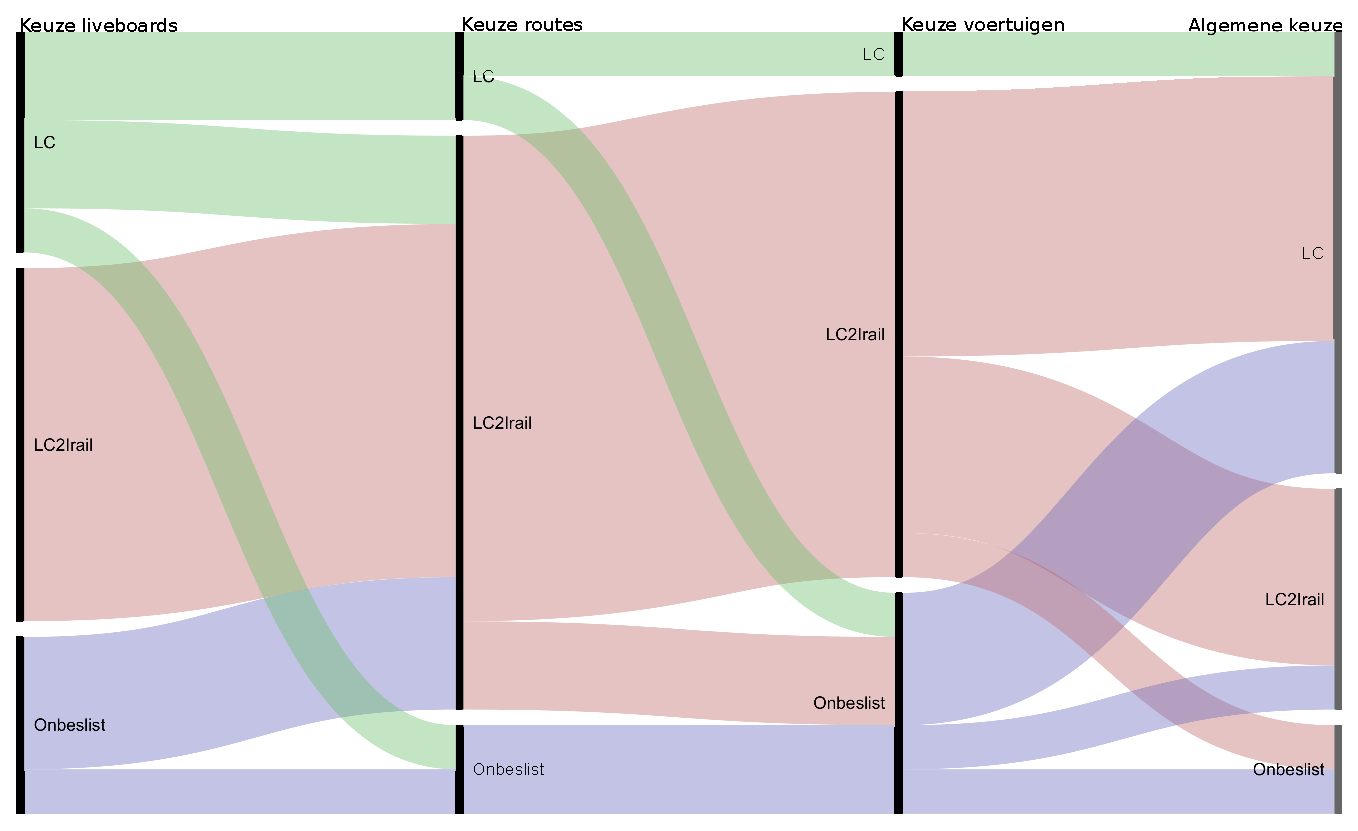
\includegraphics[width=1.00\textwidth]{alluvial_user_choice.eps}
	\caption[Door gebruikers gekozen implementatie]{Verbanden tussen de door gebruikers gekozen implementaties voor alle soorten informatie, alsook de resulterende keuze waarbij ook offline toegang in rekening werd gebracht. }
	\label{fig:alluvialUserChoices}
\end{figure}

Terwijl de meerderheid van de gebruikers steeds voor LC2Irail koos, kantelt deze balans echter volledig om wanneer gebruikers worden gevraagd om met alle aspecten rekening te houden. Dit is duidelijk zichtbaar aan de rechterkant van figuur~\ref{fig:alluvialUserChoices}. Hieruit blijkt duidelijk dat gebruikers enige snelheid willen opgeven in ruil voor offline opzoekingen. Zeven gebruikers laten weten dat ze een hybride systeem ideaal zou zijn, waarbij de snelheid van LC2Irail gecombineerd wordt met Linked Connections als offline alternatief. Wanneer deze gebruikers alsnog verplicht werden te kiezen, waren hun keuzes gelijk verdeeld, afhankelijk van de persoonlijke nood om offline te kunnen opzoeken. 


We trachten nu een antwoord te vinden op de in hoofdstuk~\ref{chap:onderzoek} gestelde vragen omtrent de gebruikerservaring.
\begin{itemize}
	\item Ervaart de gebruiker een app die lokaal Linked Connections gebruikt als sneller dan een app die gebruik maakt van een RPC API?\\
	De ervaring van de gebuiker hangt sterk af van het gebruikte toestel en de gemaakte opzoekingen. Enkel gebruikers van snelle toestellen ervaren Linked Connections in sommige gevallen als sneller. Voor liveboards is Linked Connections concurrentieel, maar voor andere opzoekingen is deze techniek meestal trager dan de gebruikte RPC API.
	\item Ervaart de gebruiker een app die lokaal Linked Connections gebruikt als sneller dan zijn huidige app?\\
	Een minderheid ervaart Linked Connections als sneller dan de huidige gebruikte applicatie. Voor liveboards, routes en voertuigen vinden respectievelijk 45\%, 30\% en 24\% dat Linked Connections sneller is. Respectievelijk 30\%, 40\% en 60\% van de gebruikers ervaren Linked Connections als even snel, met 24\%, 30\% en 12\% van de gebruikers die Linked Connections expliciet als trager ervaren dan hun huidige applicatie. Linked Connections brengt op dit moment zeker geen verbetering in snelheid voor de gebruikers.
\end{itemize}

Wat dit wilt zeggen voor de onderzoeksvraag en hypotheses en zullen we verder bespreken in hoofdstuk~\ref{chap:interpretatie}.

\section{Enquête}
Zoals vermeld in hoofdstuk~\ref{chap:onderzoek}, trachten we een aantal vragen te beantwoorden aan de hand van een enquête (bijlage~\ref{appendix:enquete}). We zullen nu eerst de resultaten van deze enquête overlopen, alvorens aan de hand van deze resultaten een antwoord te zoeken op de in hoofdstuk~\ref{chap:onderzoek} geformuleerde vragen.

\subsection{Antwoorden van respondenten}
Er werden in totaal 81 volledig ingevulde enquêtes digitaal verzameld, in een gevarieerd publiek. Zo neemt meer dan de helft van de respondenten meerdere keren per week (26\%) of dagelijks (28\%) de trein. Ook personen die occasioneel reizen zijn goed vertegenwoordigt, zo reist 16\% minder dan één keer per maand per trein.

Wanneer we kijken naar de informatiebronnen voor reizigers, blijkt dat \foreign{native} applicaties voorop staan (93\%, waarvan 27\% third-party applicaties zijn), gevolgd door digitale informatieborden en affiches (74\%) en websites (62\%) . Hierbij moeten we opmerken dat de enquête specifiek gericht is op personen die applicaties gebruiken om informatie op te zoeken, en het werkelijk aandeel van de reizigers die applicaties gebruikt dus iets lager kan liggen.

Iets minder dan de helft (48\%) van de treinreizen verloopt probleemloos. Alle respondenten geven aan vertragingen te ervaren bij het reizen, waarbij 33\% aangeeft dat dit zelfs meestal of altijd het geval is. Na vertragingen zijn spoorwijzigingen de tweede grootste bron van ergernis: meer dan 85\% van de gebruikers ervaart dit wel eens, waarbij dit voor 15\% van de reizigers regelmatig voorvalt. Tot slot geeft 72\% van de respondenten aan wel eens een afgeschafte trein te hebben, al gebeurt dit voor slechts 1\% de helft van de tijd.

Wanneer we nagaan hoe up-to-date informatie voor reizigers is, wordt duidelijk dat hier zeker ruimte is voor verbetering: slechts 25\% zegt altijd over actuele informatie in de stations te beschikken, applicaties doen het iets beter, waarbij 40\% van de gebruikers altijd over actuele informatie beschikt. Voor beide blijkt dat 50\% van de personen die dit ervaart, er slechts soms last van heeft. Echter blijkt wel dat 27\% van de personen minstens de helt van de tijd dit probleem in stations ervaart. Applicaties doen het iets beter, waar slechts 10\% van de gebruikers dit probleem minstens de helft van de tijd ervaart. Uit deze cijfers kunnen we concluderen dat gebruikers wel degelijk nood hebben aan actuele informatie. 

Applicaties blijken ook de voornaamste bron van informatie te zijn voor gebruikers: Voor alle problemen, op spoorwijzigingen na, checken gebruikers hun smartphone. Voor spoorwijzigingen blijft informatie in de stations zelf, zoals omgeroepen informatie of digitale borden populairder. Ook wanneer informatie in de applicatie niet actueel is zoeken mensen hun toevlucht tot de omgeroepen informatie of digitale borden. Wanneer gebruikers gevraagd worden om informatiebronnen naar gebruik te rangschikken, blijven applicaties en websites ook hier bovenaan staan.

Wanneer we nu gaan kijken naar de tevredenheid, blijkt dat applicaties hier uitzonderlijk goed scoren: meer dan 77\% van de gebruikers is hierover tevreden. Dit vormt een scherp contrast met websites, waar slechts 43\% tevreden over is. Voor alle informatiebronnen zijn er ontevreden gebruikers, wat er opnieuw op wijst dat er ruimte is voor verbetering.

Bij de respondenten zijn Android en iOS gelijk vertegenwoordigd, met respectievelijk 39 en 40 respondenten. Een enkele respondent gebruikt Windows Mobile, nog een enkeling gebruikt Sailfish OS. 73\% gebruikt voornamelijk de officiële NMBS applicatie, de andere 27\% is ongeveer gelijk verdeeld over third-party applicaties, zoals HyperRail, iRail, Railer en BeTrains (tesamen goed voor 21\%) en een mix van algemene en buitenlandse applicaties, zoals citymapper, de Lijn en Deutsche Bahn.

Deze applicaties gebruiken we vooral in stations (95\% van de gebruikers), maar ook thuis (85\%) en op de trein zelf (80\%). Op de trein zijn we echter niet tevreden over de snelheid waarmee resultaten laden (66\% tevreden), thuis zijn we iets tevredener (72\% tevreden). Ook de gebruiksvriendelijkheid van opzoekingen daalt tijdens het reizen. 

Naar mogelijke oorzaken van deze dalingen tijdens een reis hoeven we niet ver te zoeken: 60\% van de reizigers is ontevreden over het mobiele netwerk tijdens een treinreis. Maar liefst 96\% van de reizigers heeft last van traag of niet ladende webpagina's, de meerderheid van hun ondervind hier minstens de helft van de tijd hinder door. Diezelfde mobiele data is voor 53\% van de respondenten ook een bron van angst - ondanks dat er steeds meer data bij abonnementen geleverd wordt, blijven we schrik hebben om te veel data te verbruiken. Hier dienen we wel onmiddellijk te nuanceren: 21\% maakt zich slechts een beetje zorgen. Deze groep zal vermoedelijk vooral voorzichtig zijn met media, en niet zozeer met het gebruik van routeplanning applicaties. Vooral jongeren (jonger dan 18) en personen ouder dan 35 jaar zijn voorzichtig met hun mobiele data.

Wanneer we informatie niet opzoeken via de app, is dit voornamelijk omdat de gebruiker geen mobiele data heeft (33\%), omdat het opzoeken te lang doet (24\%), of omdat informatie in het station handiger is. We maken ons iets meer zorgen om het batterijgebruik van de applicatie (19\%) dan om het dataverbruik (15\%).

Wanneer gebruikers gevraagd wordt naar wat ze belangrijk vinden in een applicatie voor openbaar vervoer, komt het snel laden van resultaten overduidelijk op de eerste plaats. Dit wordt gevolgd door offline zoekopdrachten, waarna privacy, batterijgebruik en dataverbruik kort op elkaar volgen.

Ondanks dat privacy een hot topic is, geeft 53\% van de gebruikers aan zich hier geen zorgen om te maken. Dit zouden we misschien beter wel doen, want 75\% weet niet zeker of zijn of haar reisplannen over internet verstuurd worden, terwijl alle applicaties dit op dit moment doen. 12\% is er zelfs zeker van overtuigd dat zijn of haar reisplannen niet over internet verzonden worden. Ook over het versturen van onze locatie zijn we slecht geïnformeerd. Zo meent 17\% onterecht dat zijn of haar exacte locatie waarschijnlijk niet over internet verstuurd wordt. Voor third-party apps waarvan we zeker weten dat ze de locatie niet over internet versturen, blijkt dan weer dat verschillende personen onterecht denken dat hun locatiegegevens toch verstuurd worden. 

Terwijl de meerderheid aangaf niet wakker te liggen van hun privacy bij routeplanning applicaties, blijkt toch dat het 85 en 77 percent van de respondenten zou storen moesten respectievelijk hun locatie en reisplannen over internet verstuurd worden.
 
Overstappen naar een andere applicatie is voor velen echter een brug te ver: slechts 35 en 37 percent van de respondenten zou overstappen naar een applicatie die respectievelijk hun reisplannen en locatie niet over internet verstuurd. Een ongeveer even groot aandeel geeft aan dat ze dit misschien zouden doen, afhankelijk van wat de alternatieven zijn. Deze aantallen dienen we ook onmiddellijk te nuanceren: ondanks recente privacyschandalen, blijft het overgrote deel van de smartphonegebruikers messaging apps als Facebook Messenger en Whatsapp gebruiken, ondanks de beschikbaarheid van veiligere en privacyvriendelijkere applicaties. Overstappen en wennen aan een nieuwe applicatie kost moeite en tijd, wat veel gebruikers er niet voor over hebben.

Tot slot werden gebruikers bevraagd naar wat ze vinden van een applicatie op basis van Linked Connections. Twee personen gaven aan de uitleg niet volledig te begrijpen, en zijn van deze analyse uitgesloten.
Respondenten werden gevraagd om de vier voornaamste voordelen van Linked Connections voor gebruikers van meest naar minst belangrijk te ordenen. Ondanks dat de gebruikers geïnformeerd werden dat Linked Connections volledige privacy biedt, en dat ongeveer een derde aan gaf over te stappen naar een privacyvriendelijke applicatie, komt privacy slechts bij 15\% op de eerste plaats, en bij meer dan de helft zelfs op de vierde plaats. Snelheid blijft koploper, gevolgd door offline zoeken, aangepaste routes en tot slot privacy.

Dat aanpassen van routeplanning en privacy slechts op de vierde plaats komen wilt niet zeggen dat men dit niet belangrijk vindt. Tijdens user-tests gaven testers reeds aan deze rangschikkingen moeilijk te vinden, en wanneer gepolst wordt naar de interesse in afzonderlijke aspecten, blijkt dat mensen vooral het aanpassen van routeplanning en offline zoeken enorm interessant vinden, gevolgd door snelheid en privacy. Bij het aanpassen van routeplanning willen reizigers vooral kunnen zoeken naar routes met een kortere overstaptijd, drukke treinen mijden, en routes plannen met wat meer tijd om over te stappen. Privacy, wat op de laatste plaats staat, blijft interessant voor 83\% van de respondenten. Hieruit kunnen we besluiten dat Linked Connections enorm veel potentieel heeft voor mobiele applicaties. We zullen deze resultaten nog verder bespreken in hoofdstuk~\ref{chap:interpretatie}.

\subsection{Conclusies op basis van de enquête}
We zullen nu een antwoord formuleren op de in hoofdstuk~\ref{chap:onderzoek} geformuleerde vragen.
\begin{itemize}
	\item Bied offline informatie een meerwaarde voor gebruikers?\\
	Ja, gebruikers hebben grote interesse in offline opzoekingen, voornamelijk door een slechte mobiele internetverbinding tijdens het reizen, en in mindere mate omdat ze vrezen te veel data te verbruiken of gewoonweg niet over mobiel internet beschikken.
	\item Hecht de gebruiker belang aan privacy bij het gebruik van routeplanning apps? Zo ja, in welke mate?\\
	De gebruiker hecht in beperkte mate belang aan zijn of haar privacy bij gebruik van routeplanning apps. De helft zegt zich hier geen zorgen over te maken, maar slechts een minderheid van de gebruikers weet welke data over internet verzonden wordt. Een derde van de gebruikers zou overstappen naar apps die privacyvriendelijker zijn.
	\item Heeft de gebruiker schrik om te veel mobiele data te verbruiken?\\
	Ongeveer de helft van de gebruikers heeft schrik om te veel mobiele data te gebruiken, al maakt slechts een derde van de gebruikers zich hier ernstig zorgen om.
	\item Hecht de gebruiker belang aan dataverbruik bij het gebruik van routeplanning apps?\\
	Één op zes gebruikers geeft aan soms geen informatie met een applicatie op te zoeken uit vrees te veel data te verbruiken. Wanneer gebruikers echter gevraagd wordt om een aantal aspecten van een routeplanning applicatie van belangrijk naar onbelangrijk te rangschikken, eindigt dataverbruik op de laatste plaats. Dataverbruik is voor de gebruiker dus van ondergeschikt belang aan de functionaliteit.
	\item Is de gebruiker tevreden met de snelheid van zijn huidige routeplanning app?\\
	Thuis zijn zeven op tien gebruikers tevreden met de snelheid van routeplanning applicaties. Onderweg daalt dit tot een derde, hoogstwaarschijnlijk door slechte netwerkverbindingen.
	\item Wat is voor een gebruiker belangrijk in routeplanning apps?\\
	Gebruikers vinden vooral het snel laden van resultaten belangrijk. Na snelheid volgen offline zoekopdrachten, waarna privacy, batterijgebruik en dataverbruik ongeveer even belangrijk zijn.
	\item Is de gebruiker geïnteresseerd in routeplanning op maat? Zo ja, welke aspecten spreken hem dan aan?\\
	De gebruiker is zeer geïnteresseerd in routeplanning op maat, waarbij vooral het aanpassen van de overstaptijd in stations belangrijk is, en ook het mijden van drukke treinen als zeer interessant beschouwd wordt.
	\item Is de gebruiker geïnteresseerd in offline opzoekingen?\\
	Zoals eerder vermeld vormen offline opzoekingen een meerwaarde voor gebruikers. Wanneer expliciet bevraagd, blijkt dan ook dat veel gebruikers hier in grote mate in geïnteresseerd zijn.
	\item Is de gebruiker geïnteresseerd in de mogelijke snelheid die Linked Connections biedt?\\
	Ondanks dat veel gebruikers al tevreden zijn met de huidige snelheid van routeplanning applicaties, blijft het overgrote deel geïnteresseerd in het verder versnellen van deze applicaties.
	\item Is de gebruiker geïnteresseerd in de volledige privacy die Linked Connections biedt?\\
	Ondanks dat privacy steevast onderaan de lijst met prioriteiten van gebruikers staat, wilt dit niet zeggen dat gebruikers hierin niet geïnteresseerd zijn. Meer dan acht op tien gebruikers vindt dit interessant.
\end{itemize}

\section{Dataverbruik}
Zoals eerder aangehaald is op mobiele toestellen niet enkel de snelheid, maar ook andere zaken zoals batterijverbruik en connectiviteit van belang. We gaan nu dieper in op het dataverbruik van de applicatie. 

\begin{figure}[ht]
	\centering
	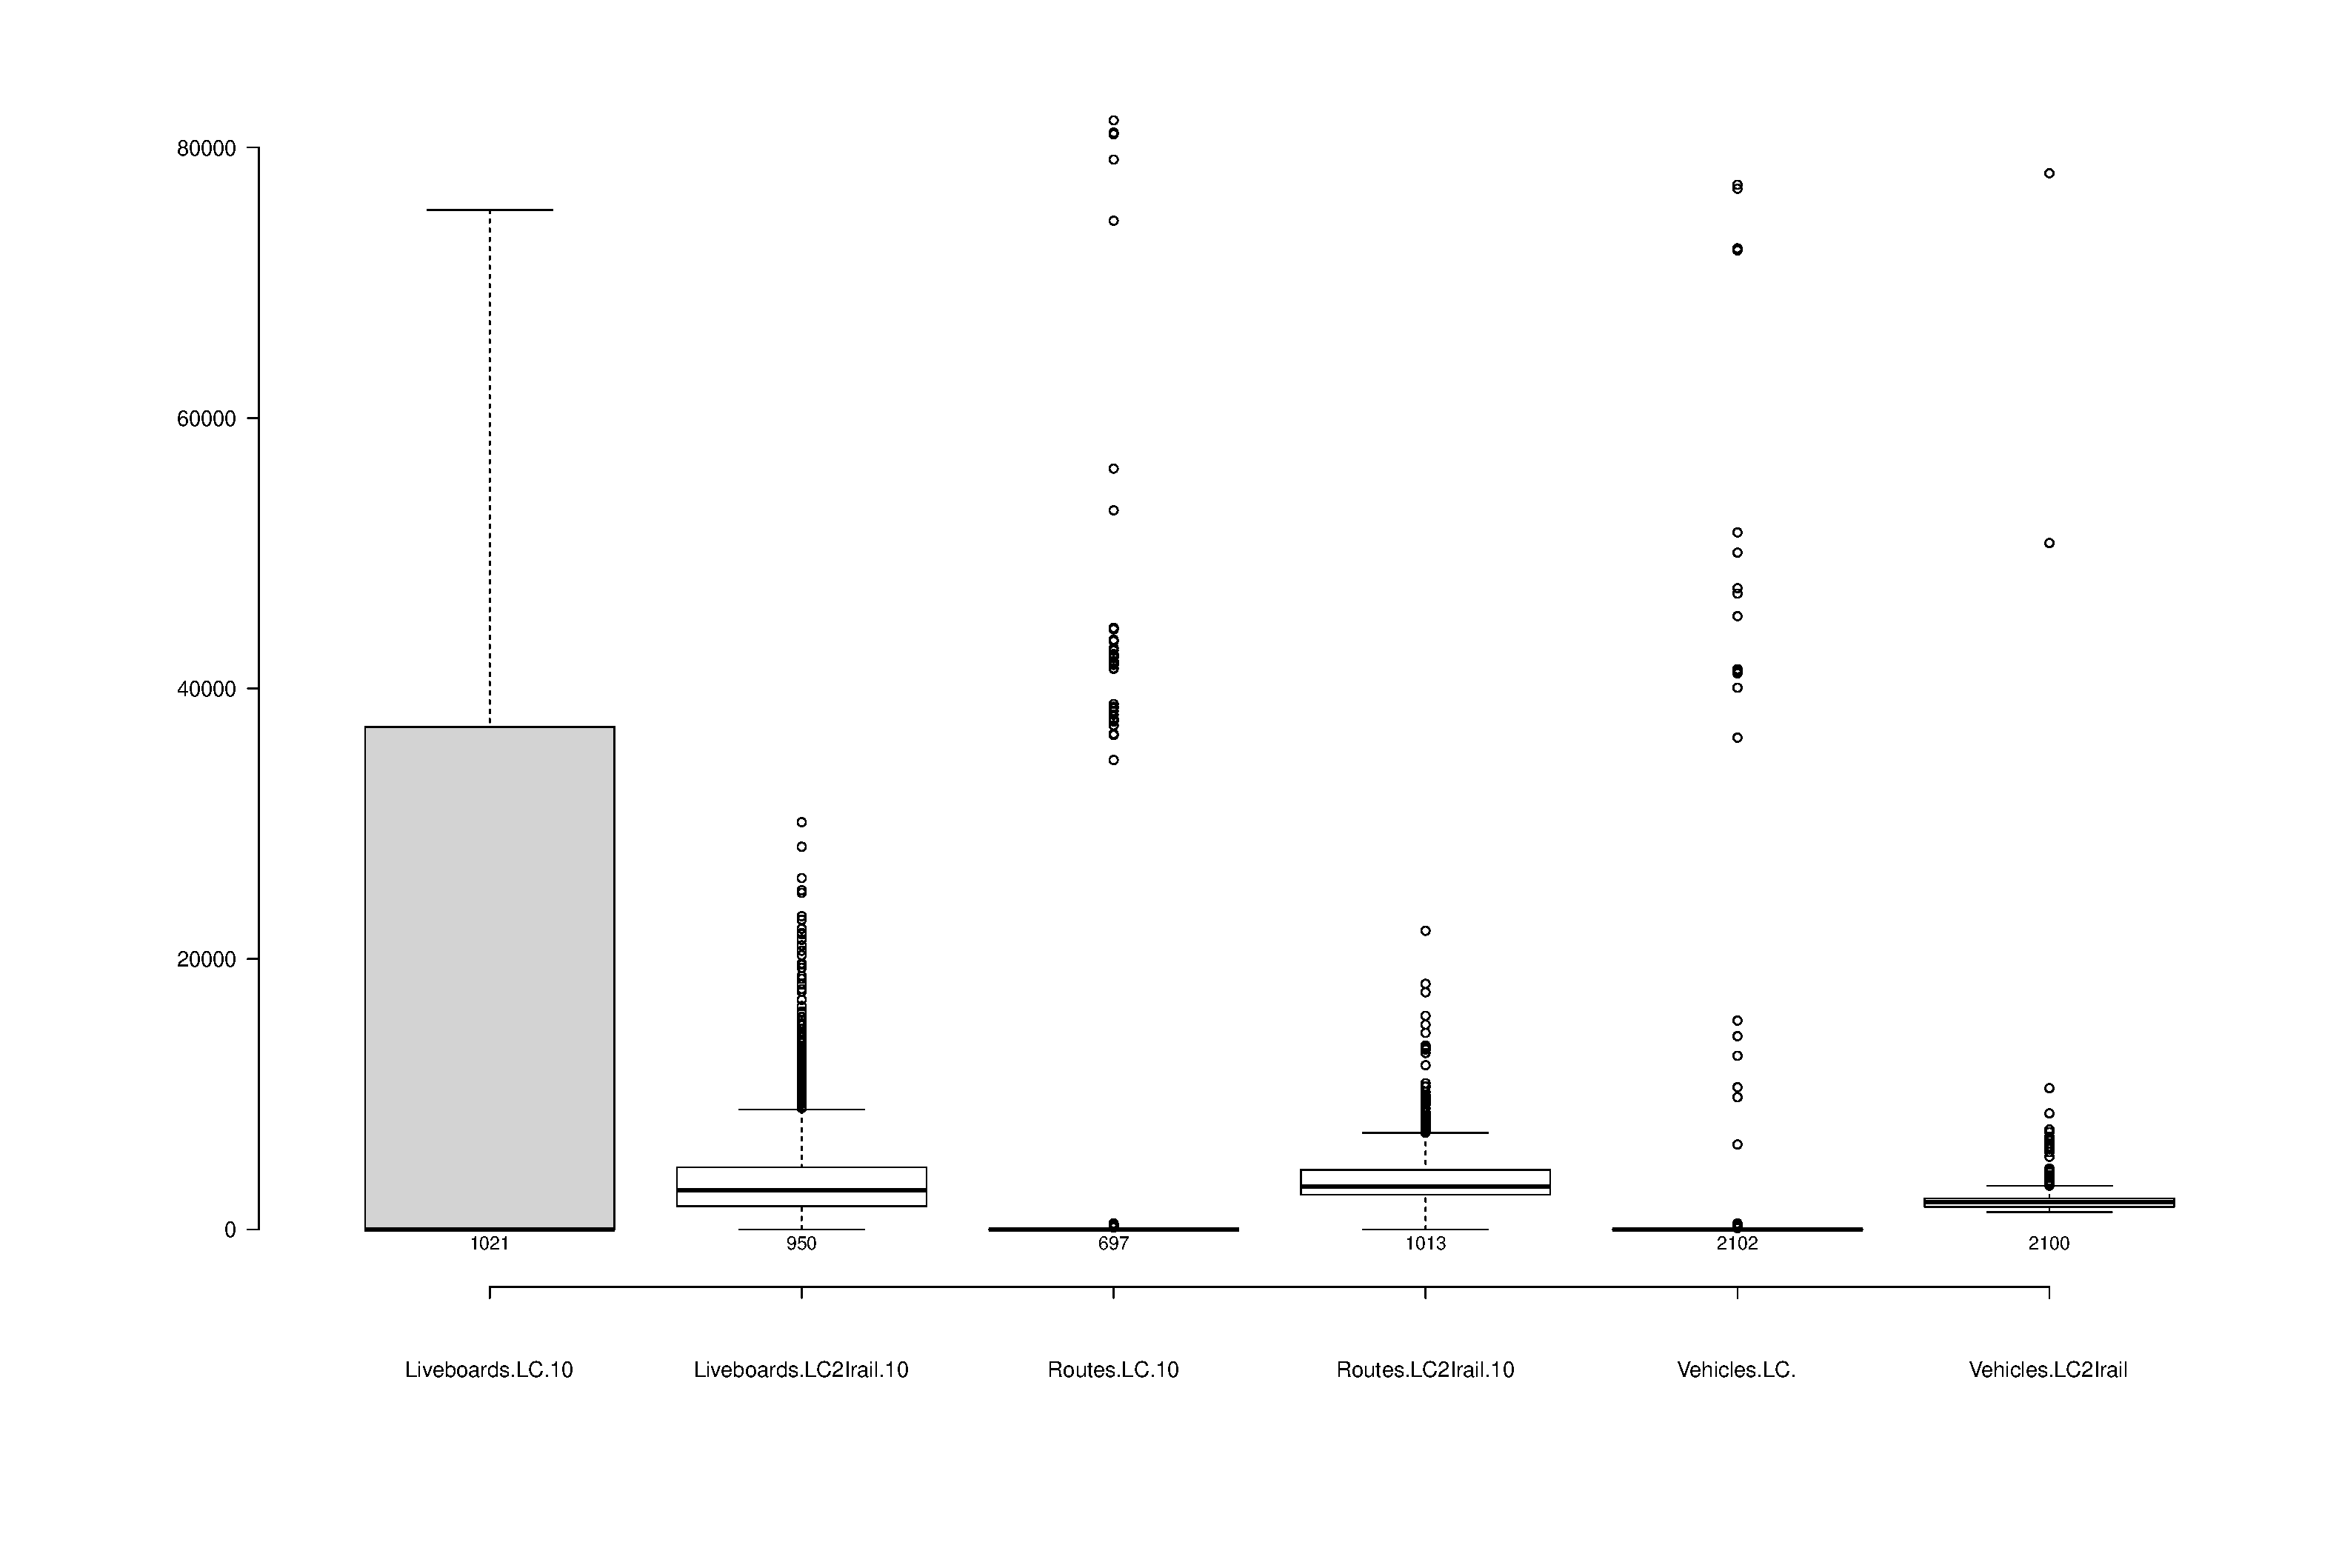
\includegraphics[width=1.00\textwidth]{dataverbruik.eps}
	\caption[Dataverbruik per opzoeking]{Dataverbruik per type opzoeking en techniek}
	\label{fig:dataUsage}
\end{figure}

Wanneer we dit dataverbruik onderzoeken, zichtbaar in figuur~\ref{fig:dataUsage}, zien we dat Linked Connections zoals te verwachten meer data gebruikt in de slechtste gevallen. Wat echter ook opvalt, is dat de mediaan steevast nul is. Dit is een rechtstreeks gevolg van de enorme cachebaarheid van Linked Connections. Linked Connections heeft ook last van grote uitlopers wanneer informatie wordt opgezocht met betrekking tot stations met weinig stops. In deze gevallen is het mogelijk dat Linked Connections alle vertrekken voor de komende paar dagen op moet halen, terwijl LC2Irail niet meer data dan anders moet versturen. LC2Irail zal immers steeds minstens één resultaat teruggeven, waardoor in het slechtste geval 10 verzoeken nodig zijn. Linked Connections kent geen harde bovengrens voor het aantal verzoeken, al is het zinloos om langer dan 15 seconden te zoeken~\citep{miller68}.

In het geval van Linked Connections zien we duidelijke verschillen tussen het opzoeken van liveboards en andere types data. Dit is te verklaren door het feit dat om een liveboard van een station te reconstrueren vaak slechts één of twee pagina's nodig zijn. Hierdoor is minder data nodig, maar wordt ook minder data gecachet. Opzoekingen voor verschillende tijdstippen hebben verschillende data nodig, terwijl deze nog niet gecachet is, waardoor minder vaak de cache gebruikt kan worden. Bijgevolg hebben meer dan 25\% van de opzoekingen nieuwe data nodig.
Wanneer we echter kijken naar dataverbruik voor routes en voertuigen, gebruiken deze verzoeken erg veel data. Hierdoor is er echt vaker een overlap tussen opzoekingen. Als gevolg wordt hier bij de enkele verzoeken enorm veel data binnengehaald, waarna vrijwel alle verzoeken uit cache beantwoord kunnen worden. We zien dat ook het derde kwartiel nul bedraagt, wat wilt zeggen dat meer dan 75\% van de verzoeken uit cache geladen kan worden. Dit laden zien we in de uitlopers, die tot 2,4 megabyte kunnen oplopen.

Door data vooraf te laden wanneer de gebruiker verbonden is via Wi-Fi, zouden we ook deze uitlopers kunnen vermijden. In dit geval zou eerst een antwoord berekend kunnen worden op basis van offline (verouderde) gegevens, waarna alle gebruikte pagina's opnieuw opgehaald worden om het actuele antwoord op te bouwen.


\begin{figure}[ht]
	\centering
	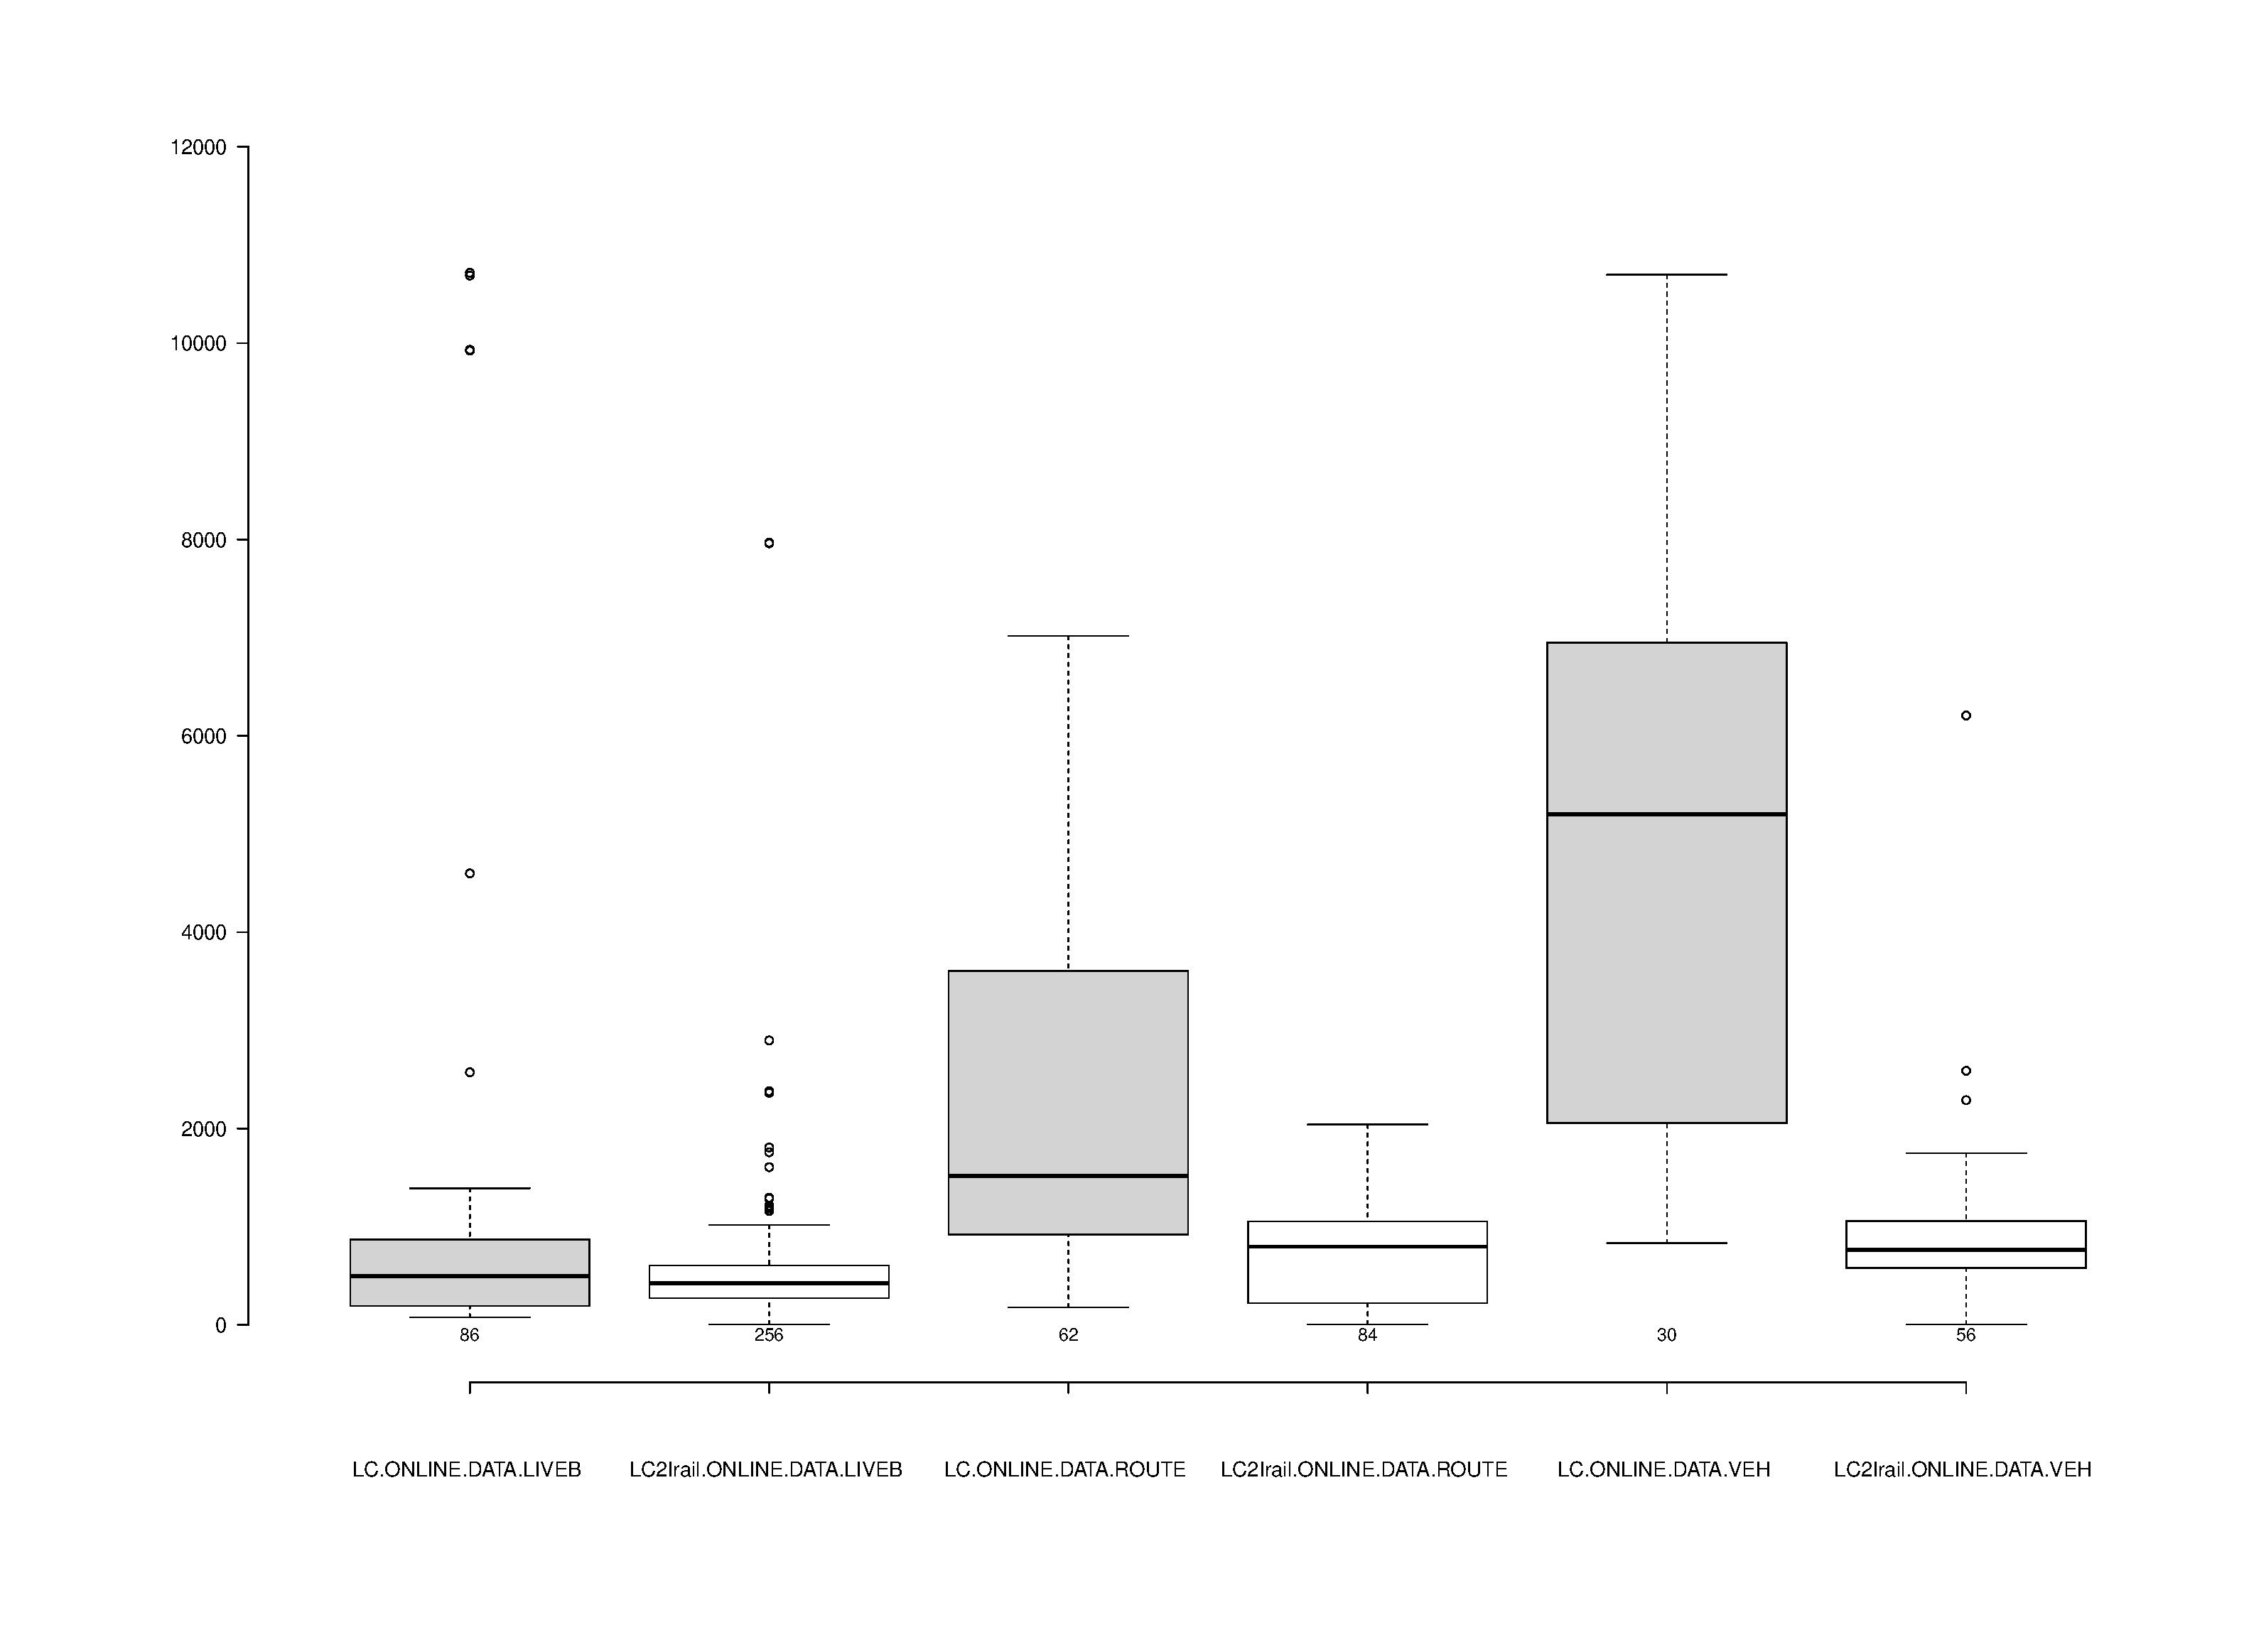
\includegraphics[width=1.00\textwidth]{dataverbruik_werkelijk.eps}
	\caption[Werkelijk dataverbruik per opzoeking Linked Connections]{Dataverbruik in werkelijke omstandigheden per type opzoeking voor Linked Connections}
	\label{fig:dataUsageRealLife}
\end{figure}

Bij deze cijfers dienen we een belangrijke kanttekening te maken. Deze gegevens tonen aan dat Linked Connections enorm cachbaar is, en enorm kan variëren in dataverbruik. Dit in tegenstelling tot Linked Connections, dat bijna altijd internet nodig heeft, met uitzondering van enkele populaire opzoekingen, die tijdens spitsuur uit cache geladen konden worden. Echter zijn deze gebaseerd op opzoekingen uitgevoerd op een server door verschillende gebruikers, en is de cache extreem afhankelijk van vorige opzoekingen. Het exacte dataverbruik wordt met andere woorden bepaald door het gebruikspatroon van de applicatie, en door eventueel gebruik van technieken zoals prefetching. Ter illustratie is in figuur~\ref{fig:dataUsageRealLife} het werkelijke dataverbruik tijdens online opzoekingen weergegeven (online opzoekingen zijn opzoekingen waarbij internet beschikbaar was, en de applicatie dus vrije keus had tussen cache en online data). In deze figuur zien we een veel realistischer beeld, waarbij dat er, ondanks dat sommige opzoekingen volledig uit cache beantwoord kunnen worden, meestal toch data opgehaald wordt. Ook bij deze grafiek plaatsen we kanttekeningen. Zo zijn de metingen voor liveboards en routes per incrementeel resultaat (er zijn dus mogelijk meerdere dergelijke opzoekingen nodig) en is het gebruik van de applicatie alsnog kunstmatig. Gebruikers kunnen in werkelijkheid mogelijk trager opzoeken, waardoor minder verzoeken uit cache beantwoord zouden kunnen worden.


\section{Batterijverbruik}
Naast dataverbruik is ook energieverbruik belangrijk bij draagbare toestellen. We gaan nu dieper in op het batterijverbruik van de applicatie. Dit is moeilijk om exact te meten, gezien alle omstandigheden exact dezelfde moeten zijn. Automatische testen op UI vereisen een USB-verbinding, waarbij stroom via USB geleverd wordt in plaats van via de batterij. 

Om toch consistent verschillende applicaties te kunnen testen, maken we een variant op de testapplicatie, waarin we knoppen plaatsen om een korte benchmark uit te voeren. Hierdoor kunnen we dezelfde test voor elk soort opzoeking uitvoeren, waarna we uit Android energiebeheer het verbruik aflezen en het toestel weer tot 100\% opladen alvorens de volgende test uit te voeren. Om aan testdata te komen kiezen we voor elk endpoint 5\% van de opzoekingen uit de iRail logs. De resultaten van deze tests zijn te zien in figuur~\ref{fig:batteryUsage}.

\begin{figure}[ht]
	\centering
	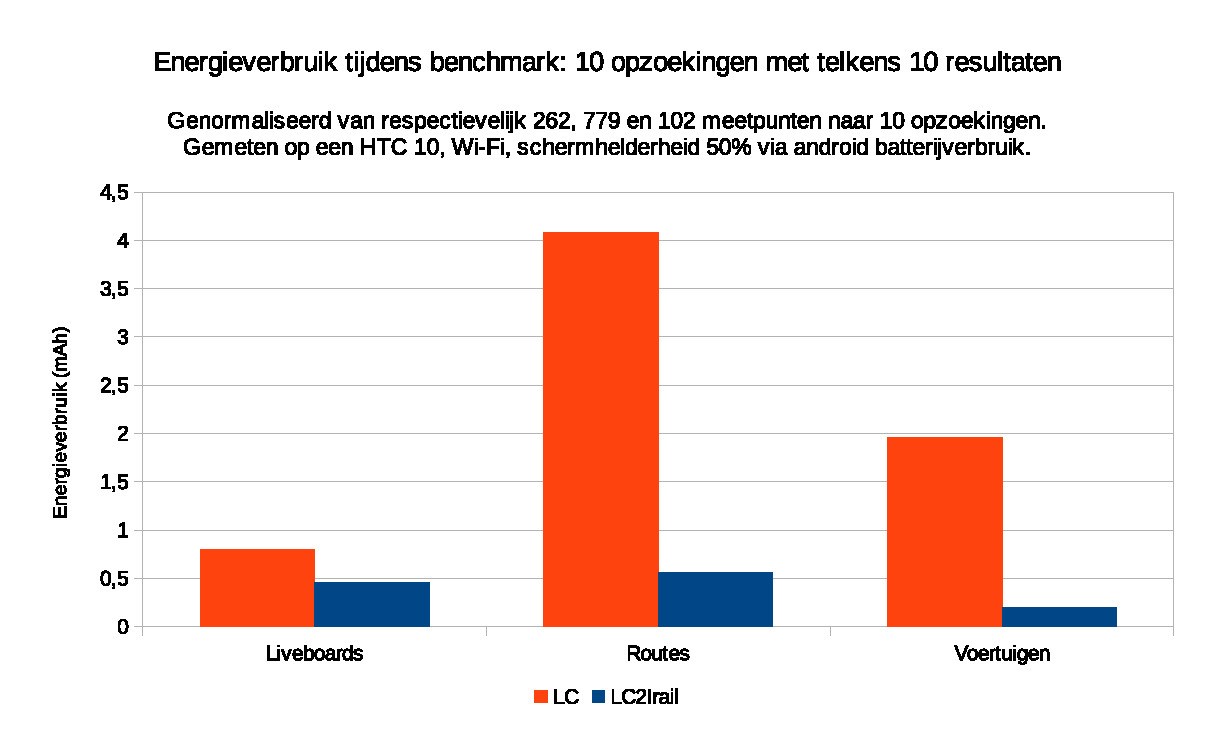
\includegraphics[width=1.00\textwidth]{energieverbruik.eps}
	\caption[Energieverbruik per opzoeking]{Gemiddeld energieverbruik per type opzoeking en techniek}
	\label{fig:batteryUsage}
\end{figure}

Onmiddellijk vallen enkele verschillen tussen beide implementaties op. Zo zien we dat Linked Connections steeds een veelvoud aan energie verbruikt. Dit varieert tussen dubbel zoveel voor Liveboards, tot acht maal zoveel voor routes. We zien hier een duidelijk verband tussen energieverbruik, de hoeveelheid gedownloade data en de complexiteit van de toegepaste algoritmes.
Liveboards, die weinig data en weinig processing vereisen, verbruiken het minst energie. Voertuigen, die meer data vereisen maar nog steeds een relatief eenvoudig algoritme hebben verbruiken ongeveer drie keer meer energie. Routes vereisen iets minder data dan voertuigen,  maar hebben een complexer algoritme. De processortijd blijkt een grote impact te hebben op de batterij, met een verdubbeling ten opzichte van het energieverbruik bij voertuigen tot gevolg.

Een belangrijke nuance bij deze resultaten is dat zelfs in het slechtste geval, het laden van routes via Linked Connections, slechts 4mAh verbruikt wordt. Dit is zeer weinig, en zal zelfs op smartphones met een zeer kleine batterij (2.000mAh) slechts 0,2\% batterij verbruiken. Op toestellen met een gemiddelde batterij (3.200mAh) zakt dit verder tot 0,125\%. Linked Connections verbruikt wel degelijk meer dan LC2Irail, maar het effect op de gebruiker blijft steeds beperkt.

\section{Beperkingen}
\label{sec:beperkingen}

Het grootste deel van deze masterproef is gebaseerd op user-testing en benchmarks van de ontwikkelde applicatie. Deze tests zijn echter aan enkele beperkingen onderhevig. Deze beperkingen hebben geen grote impact op het onderzoek en hebben geen invloed op de uiteindelijke conclusies, maar kunnen de volledigheid of precisie van het onderzoek lichtjes beïnvloeden.

\subsection{Kleine steekproef voor user-testing}
Zoals eerder vermeld ontbreekt op het moment van schrijven nog cruciale informatie in Linked Connections, zoals of een voertuig al dan niet afgeschaft is, en op welk perron een voertuig aankomt. Hierdoor moesten we terugvallen op user-testing onder begeleiding, om gebruikers aan te sporen hun gebruikelijke opzoekingen te doen en te polsen naar hun ervaringen. Dit neemt relatief veel tijd in beslag, waardoor weinig mensen én zin, én tijd hebben. Voorts neemt deze methode van testen ook veel tijd in beslag voor de onderzoeker. 

De groep testgebruikers is wel gevarieerd, zowel in persoonlijke eigenschappen zoals leeftijd, als in reisgewoontes per trein. Wanneer de gehele testgroep duidelijk de voorkeur geeft aan een bepaalde variant, kunnen we deze keuze veralgemenen naar de gehele populatie. Wanneer er echter geen grote meerderheid voor eenzelfde variant kiest, moeten we voorzichtig zijn met conclusies.

\subsection{Beperkt aantal unieke toestellen getest}
Uit de voorgaande secties blijkt dat het gebruikte toestel van groot belang is voor de prestaties van de lokale Linked Connections implementatie. Tijdens het user-testen werd gebruik gemaakt van twaalf verschillende smartphones. Dit aantal is relatief beperkt in vergelijking met het aanbod op de huidige smartphonemarkt. Eventuele verder onderzoek zal de prestaties van Linked Connections op verschillende toestellen moeten vastleggen.

\subsection{Processorverbruik niet meetbaar}
De Android CPU Profiler beïnvloed de prestaties van de applicatie zodanig dat het onmogelijk is om een correct beeld te krijgen van het processorverbruik. Er kan een beeld gevormd worden welke onderdelen van de applicatie het meest processortijd vragen, maar exacte tijdsmetingen zijn niet mogelijk. Deze problemen worden ook door andere Android ontwikkelaars op internet beschreven\footnote{\url{https://stackoverflow.com/questions/49555983/background-concurrent-copying-gc-freed}}. Deze problemen treden op door de nieuwe Android CPU profiler, die zelf teveel processortijd op het apparaat vereist.

\subsection{Prestaties zijn sterk afhankelijk van implementatiedetails}
Zoals blijkt uit grafieken %TODO: REFERENTIE
is de performantie van de lokale Linked Connections implementatie sterk afhankelijk van details in de implementatie - Het is dus niet enkel belangrijk om de algoritmes te optimalizeren, maar ook om rekening te houden met processen zoals Garbage Collection. Dit werd pas in een gevorderd stadium van de proef vastgesteld. Het is mogelijk dat de resultaten in dit onderzoek nog verder verbeterd kunnen worden door dezelfde algoritmes efficiënter te implementeren.

\subsection{Kleine afwijkingen tussen opzoekingen LC en LC2Irail}
Hoewel zowel Linked Connections en LC2Irail betrouwbaar werken in de testapplicatie, zijn er nog een beperkt aantal gevallen waarin het automatisch laden van incrementele resultaten niet werkt. Dit is onder andere mogelijk bij stations waar voor langer perioden geen voertuig stopt, of routes waarvoor slechts enkele resultaten per dag beschikbaar zijn. Om te zorgen dat ook voor deze opzoekingen incrementele resultaten feilloos laden zijn verdere verfijningen nodig aan de stopvoorwaarden en implementatie. Zo moet voorkomen worden dat er bij opzoekingen die data van meerdere dagen vereisen te veel callbacks gebruikt worden, een neveneffect dat tijdens de ontwikkeling nog niet bekend was. Aangezien enkel succesvolle opzoekingen meegenomen worden in testresultaten, is het hierdoor mogelijk dat er een klein verschil zit op het aantal meetpunten bij vergelijkende tests tussen LC en LC2Irail. Dit verschil treed vooral op bij het opzoeken van routes, en heeft geen merkbare invloed op resultaten door de grootte van de steekproef.
% !TeX spellcheck = nl_NL
\begin{savequote}[0.55\linewidth]
	``Inspirational quote''
	\qauthor{\textasciitilde Source}
\end{savequote}

\chapter{Interpretatie}
\label{chap:interpretatie}

We zullen nu de resultaten, besproken in hoofdstuk \ref{chap:resultaten}, proberen interpreteren om een antwoord te vinden op de in sectie \ref{sec:onderzoeksvraag} geuite vragen. Het is onmiddellijk duidelijk dat het moeilijk wordt hier een eenduidig antwoord op te vinden.

\paragraph{Onderzoeksvraag}  \textbf{Verbetert de user experience en user perceived perforance van een applicatie voor openbaar vervoer wanneer gebruik gemaakt wordt van Linked Connections in plaats van traditionele RPC API's?}\\

 Voor liveboards blijkt dat, afhankelijk van het gebruikte toestel Linked Connections concurrentieel is op vlak van snelheid, zowel gemeten als ervaren. Dit wordt ook duidelijk gereflecteerd in de ervaren snelheid, die door een groot deel van de gebruikers als "redelijk snel" of beter aangeduid wordt. Toch blijkt dat de ervaren snelheid iets onderdoet voor die van een RPC API.

Bij routes en voertuigen wordt de achterstand van Linked Connections tegenover RPC steeds groter. Gebruikers zijn het ook absoluut niet met elkaar eens over de ervaren snelheid, terwijl voor LC2Irail vrijwel alle gebruikers voor (ongeveer) dezelfde snelheid ervoeren.

Hieruit trekken we de conclusie dat Linked Connections enorm afhankelijk is van het gebruikte toestel,  waarbij toestellen met meer processorkracht en/of werkgeheugen een duidelijk voordeel hebben ten opzichte van toestellen die over mindere specificaties beschikken.

Hoewel Linked Connections ten opzichte van LC2Irail traag kan overkomen, dienen we dit zeker te nuanceren. Zo is LC2Irail, de gebuikte referentie voor een RPC API, beduidend sneller dan Linked Connections. Echter blijkt dat de meeste gebruikers LC2Irail als sneller ervaren in vergelijking met de huidige beschikbare applicaties, en Linked Connections in veel gevallen als even snel als beschikbare applicaties. Wel zijn de prestaties van Linked Connections incosistent en sterk afhankelijk van de gemaakte opzoeking, waardoor gebruikers sneller irritatie ervaren bij het gebruik van Linked Connections dan bij het gebruik van LC2Irail.

\textbf{De user-perceived performance van Linked Connections is algemeen gezien, voor de meerderheid van de gebruikers, gelijk of iets slechter dan de user-perceived performance van RPC API's.}

Opvallend is ook dat de meerderheid van de gebruikers, ondanks aan te geven dat ze LC2Irail sneller ervaren, toch aangeeft liefst Linked Connections te gebruiken wanneer ook offline toegang meespeelt. Dit wilt zeggen dat gebruikers Linked Connections snel genoeg ervaren om een algemene betere gebruikerservaring te bieden vergeleken met RPC API's.

\textbf{De user experience van een routeplanning applicatie op basis van Linked Connections is beter dan de user-experience van een identieke applicatie die gebruikt maakt van een RPC API, voornamelijk door een hoge betrouwbaarheid onafhankelijk van de beschikbaarheid van (mobiel) internet.}

We gaan even dieper in op de prestaties, en proberen op basis van alle voorgaande informatie de achterliggende oorzaak van de variërende prestaties. te achterhalen. Testpersonen die achtereenvolgens een implementatie op basis van de \foreign{org.json} parser en de \foreign{LoganSquare} voorgeschoteld kregen, gaven allemaal aan dat de \foreign{LoganSquare} parser betere prestaties boodt, zowel op budget- als high-end smartphones. Hierbij werd telkens gemeten hoe lang het duurde om een Linked Connections pagina van JSON om te vormen tot een object. Dit is het enige verschil tussen beide implementaties, maar toch blijkt hier dat het 50e percentiel voor de uitvoeringstijd van deze code verdubbelde bij gebruik van de \foreign{LoganSquare} parser: in plaats van 100 zijn nu 200 milliseconden nodig.

Dit is volledig tegenstrijdig aan de gebruikerservaringen, en is dan ook moeilijk te vatten. Echter is er een zeer belangrijke "externe" invloed op de uitvoeringstijd, namelijk de \foreign{Java Virtual Machine} die de applicatie uitvoert. Deze JVM pauzeert de applicatie voor \foreign{garbage collection} wanneer er te veel \foreign{garbage} is - objecten die ooit gebruikt werden, maar waar nu geen enkele verwijzing meer naar bestaat. Tijdens deze \foreign{garbage collection} worden alle ongebruikte objecten verwijderd om geheugen vrij te maken. Hierbij komt het voordeel van de \foreign{LoganSquare} parser naar boven: ondanks dat het parsen op zich langer duurt, wordt aanzienlijk minder \foreign{garbage} gecreëerd, en is het aanzienlijk minder vaak nodig om de applicatie te pauzeren voor \foreign{garbage collection}.

Hierbij komt ook nog dat toestellen die over minder processorkracht beschikken, ook vaak over minder geheugen beschikken. Hierbij kunnen fabrikanten kiezen om de \foreign{garbage collection} agressiever in te stellen, wat leid tot efficienter geheugengebruik ten koste van prestaties. %TODO: citation needed
Elke garbage collection zal door de beperktere processorkracht ook meer tijd vereisen, waardoor de applicatie niet alleen meer, maar ook langer gepauzeerd wordt. Hierdoor weegt Linked Connections extra zwaar door op trage toestellen: niet alleen kosten de algoritmes meer tijd, maar ook parsen van JSON kost meer tijd. Tragere modems kunnen er verder nog voor zorgen dat ook het netwerk verkeer trager gaat. Al deze factoren maken dat Linked Connections enorm afhankelijk is van het gebruikte toestel en de gebruikte programmeertaal, terwijl een RPC API zoals LC2Irail slechts weinig data over het netwerk verzend, een klein antwoord heeft wat niet tot \foreign{garbage collection} leidt, en geen verdere algoritmes of verwerking vereist aan de client side. 

Het zou onterecht zijn om Linked Connections definitief als "slechter" te bestempelen. Wel kunnen we zeggen dat er zeer veel aandacht aan de exacte implementatie besteed moet worden, waarbij ontwikkelaars diepgaande kennis over hun omgeving moeten beschikken. Een ontwikkelaar die geen kennis heeft van de principes van \foreign{garbage collection}, zal sneller problemen ervaren bij de performantie van Linked Connections dan bij het implementeren van een RPC API.

\paragraph{Hypothese 1} \textbf{Ervaart de gebruiker de mogelijkheid voor offline zoekopdrachten als een meerwaarde?}
	Gebruikers hebben grote interesse in offline opzoekingen, voornamelijk door een slechte mobiele internetverbinding tijdens het reizen, en in mindere mate omdat ze vrezen te veel data te verbruiken of gewoonweg niet over mobiel internet beschikken.
	
\textbf{Hieruit volgt dat Hypothese 1 correct is, en de gebruiker dit inderdaad als meerwaarde ervaart.
}
\paragraph{Hypothese 2}\textbf{ Ervaart de gebruiker de mogelijkheid om voorkeuren voor routes in te stellen (overstaptijd, toegankelijkheid, ...) als een meerwaarde?}
	De gebruiker is zeer geïnteresseerd in routeplanning op maat, waarbij vooral het aanpassen van de overstaptijd in stations belangrijk is, en ook het mijden van drukke treinen als zeer interessant beschouwd wordt.

	\textbf{Hieruit volgt dat Hypothese 2 correct is, en de gebruiker dit inderdaad als meerwaarde ervaart. }	
\paragraph{Hypothese 3}\textbf{ Heeft de gebruiker angst om te veel mobiele data te verbruiken, en let deze hier op bij het gebruik van routeplanning-apps?}
    53\% van de gebruikers is nog voorzichtig met zijn of haar databundel. Slechts 14\% heeft redelijk veel schrik om te veel data te verbruiken, 19\% heeft veel of enorm veel schrik om te veel data te verbruiken. Gebruikers zijn dus zeker nog voorzichtig met hun databundel, al maakt 47\% zich hier absoluut geen zorgen over.
    Wanneer we kijken naar datagebruik bij routeplanning applicaties, blijkt dat één op zes gebruikers soms geen informatie met een applicatie op te zoeken uit vrees te veel data te verbruiken. Dit komt ongeveer overeen met de personen die aangaven nog veel schrik te hebben om te veel data te verbruiken.
    
    Wanneer gebruikers echter gevraagd wordt om een aantal aspecten van een routeplanning applicatie van belangrijk naar onbelangrijk te rangschikken, eindigt dataverbruik op de laatste plaats. Dataverbruik is voor de gebruiker dus van ondergeschikt belang aan de functionaliteit.
    
    \textbf{De helft van de gebruikers heeft angst om te veel mobiele data te gebruiken, maar slechts één op zes gebruikers let ook op bij het gebruik van routeplanning applicaties op mobiel datagebruik. Hypothese 3 blijkt correct.}
\paragraph{Hypothese 4}\textbf{Ervaart de gebruiker extra privacy bij het opzoeken van routes niet als een noemenswaardige meerwaarde?}
	Gebruikers maken zich niet echt zorgen om hun privacy bij het gebruik van routeplanning applicaties. Verder zijn ze ook zeer slecht op de hoogte welke data over internet verzonden wordt. Privacy belandt ook steevast onderaan de lijst met prioriteiten voor gebruikers. Dit wilt echter niet zeggen dat men hierin niet geïnteresseerd is. Wanneer expliciet naar interesse om meer privacy gepolst wordt, geeft meer dan acht op tien gebruikers aan dit interessant te vinden.
	
	\textbf{Gebruikers ervaren extra privacy als een meerwaarde, alhoewel deze niet noemenswaardig is, en niet noemenswaardig veel gebruikers zal overhalen over te stappen? Ook hypothese 4 blijkt correct.}
\bibliography{referenties}

\begin{appendices}
	
\chapter{Codefragmenten}
\label{appendix:code}


\begin{listing}[h]
	\begin{minted}[breaklines,tabsize=2]{java}
	if (T3_transferArrivalTime.getMillis() <= T2_stayOnTripArrivalTime.getMillis()) {
	Tmin = T3_transferArrivalTime;
	exitTrainConnection = connection;
	numberOfTransfers = T3_transfers;
	} else {
	Tmin = T2_stayOnTripArrivalTime;
	if (T2_stayOnTripArrivalTime.isBefore(infinite)) {
	exitTrainConnection = T.get(connection.trip).arrivalConnection;
	} else {
	exitTrainConnection = null;
	}
	numberOfTransfers = T2_transfers;
	}
	
	// For equal times, prefer just arriving.
	if (T1_walkingArrivalTime.getMillis() <= Tmin.getMillis()) {
	Tmin = T1_walkingArrivalTime;
	exitTrainConnection = connection;
	numberOfTransfers = T1_transfers;
	}
	
	if (Tmin.isEqual(infinite)) {
	continue;
	}
	\end{minted}
	\caption[CSA: Bepalen van vroegste aankomsttijd]{Bepalen van de vroegste aankomsttijd bij het evalueren van een nieuwe connectie.}
	\label{code:2:csaMin}
\end{listing}

\begin{listing}[h]
	\begin{minted}[breaklines,tabsize=2]{java}
	if (Tmin.isEqual(T.get(connection.getTrip()).arrivalTime)
	&& !T.get(connection.getTrip()).arrivalConnection.getArrivalStationUri()
	.equals(mRoutesRequest.getDestination().getUri())
	&& T3_transferArrivalTime.isEqual(T2_stayOnTripArrivalTime)
	&& S.containsKey(T.get(connection.getTrip()).arrivalConnection.getArrivalStationUri())
	&& S.containsKey(connection.getArrivalStationUri())
	) {
	LinkedConnection currentTrainExit = T.get(connection.getTrip()).arrivalConnection;
	
	StationStopProfile stationStopProfile = new StationStopProfile();
	stationStopProfile.departureTime = connection.getDepartureTime();
	stationStopProfile.departureConnection = connection;
	
	stationStopProfile.arrivalTime = Tmin;
	stationStopProfile.arrivalConnection = currentTrainExit;
	
	Duration currentTransfer = new Duration(currentTrainExit.getArrivalTime(), getFirstReachableConnection(stationStopProfile).departureTime);
	
	// New situation
	stationStopProfile.arrivalTime = Tmin;
	stationStopProfile.arrivalConnection = exitTrainConnection;
	Duration newTransfer = new Duration(exitTrainConnection.getArrivalTime(), getFirstReachableConnection(stationStopProfile).departureTime);
	
	// If the new situation is better
	if (newTransfer.isLongerThan(currentTransfer)) {
	TrainProfile trainProfile = new TrainProfile();
	trainProfile.arrivalTime = Tmin;
	trainProfile.arrivalConnection = exitTrainConnection;
	trainProfile.transfers = numberOfTransfers;
	
	T.put(connection.getTrip(), trainProfile);
	}
	}
	
	if (Tmin.isBefore(T.get(connection.getTrip()).arrivalTime)) {
	TrainProfile trainProfile = new TrainProfile();
	trainProfile.arrivalTime = Tmin;
	trainProfile.arrivalConnection = exitTrainConnection;
	trainProfile.transfers = numberOfTransfers;
	
	T.put(connection.getTrip(), trainProfile);
	}
	\end{minted}
	\caption[CSA: Bijwerken T]{Bijwerken van de trips gegevensstructuur.}
	\label{code:2:csaT}
\end{listing}

\begin{listing}[h]
	\begin{minted}[breaklines,tabsize=2]{java}
	StationStopProfile newProfile = new StationStopProfile();
	newProfile.departureTime = connection.getDepartureTime();
	newProfile.arrivalTime = Tmin;
	newProfile.departureConnection = connection;
	newProfile.arrivalConnection = T.get(connection.getTrip()).arrivalConnection;
	newProfile.transfers = numberOfTransfers;
	if (S.containsKey(connection.getDepartureStationUri())) {
	int numberOfPairs = S.get(connection.getDepartureStationUri()).size();
	StationStopProfile existingProfile = S.get(connection.getDepartureStationUri()).get(numberOfPairs - 1);
	
	if (newProfile.arrivalTime.isBefore(existingProfile.arrivalTime)) {
	if (newProfile.departureTime.isEqual(existingProfile.departureTime)) {
	S.get(connection.getDepartureStationUri()).remove(numberOfPairs - 1);
	S.get(connection.getDepartureStationUri()).add(numberOfPairs - 1, newProfile);
	} else {
	S.get(connection.getDepartureStationUri()).add(newProfile);
	}
	}
	} else {
	S.put(connection.getDepartureStationUri(), new ArrayList<StationStopProfile>());
	S.get(connection.getDepartureStationUri()).add(newProfile);
	}
	\end{minted}
	\caption[CSA: Bijwerken S]{Bijwerken van de stops gegevensstructuur.}
	\label{code:2:csaS}
\end{listing}

\begin{listing}[h]
	\begin{minted}[breaklines,tabsize=2]{java}
	Route[] routes = new Route[S.get(mRoutesRequest.getOrigin().getSemanticId()).size()];
	
	int i = 0;
	for (StationQuintuple quint : S.get(mRoutesRequest.getOrigin().getSemanticId())
	) {
	// it will iterate over all legs
	StationQuintuple it = quint;
	List<RouteLeg> legs = new ArrayList<>();
	
	while (!Objects.equals(it.arrivalConnection.arrivalStationUri, mRoutesRequest.getDestination().getSemanticId())) {
	// use it.departureConnection and it.arrivalConnection to construct legs of this journey
	legs.add(...);
	it = getFirstReachableConnection(it);
	}
	
	routes[i++] = new Route(legs);
	}
	\end{minted}
	\caption[CSA: Journey extraction]{Journey Extraction door middel van post-processing.}
	\label{code:2:csaJourneyExtraction}
\end{listing}	

\chapter{Vragen enquete}
\label{appendix:enquete}

\begin{itemize}
	
	
	\item Hoe vaak neem je de trein?
	\item In welk(e) verband(en) neem je de trein?
	\item Waar haal je (realtime) informatie met betrekking tot treinen vandaan?
	\item Hoe vaak ervaar je volgende gebeurtenissen wanneer je met de trein reist, en waar zoek je in deze gevallen informatie op?
	\begin{itemize}
		\item Een probleemloze rit
		\item Vertraging
		\item Afgeschafte treinen
		\item Spoorwijzigingen
		\item Informatie in stations niet up-to-date
		\item Informatie in app niet up-to-date
	\end{itemize}
	
	\item Hoe tevreden ben je over informatiebronnen voor openbaar vervoer per trein?
	\item Rangschik deze bronnen voor informatie voor openbaar vervoer per trein naar hoe vaak je ze gebruikt, van meest naar minst gebruikt.
	\begin{itemize}
		\item Website
		\item App
		\item Affiches of digitale borden in station
		\item Loketten
		\item Omgeroepen informatie
	\end{itemize}
	
	\item Welk besturingssysteem gebruik je op je (meestgebruikte) smartphone
	\item Welke app gebruik je hoofdzakelijk?
	\item Waar gebruik je deze app?
	\item Hoe tevreden ben je over de volgende zaken wanneer je je applicatie gebruikt?
	\item Hoe tevreden ben je over het mobiele netwerk tijdens een treinreis?
	\item Heb je soms last van een zeer trage of afwezige netwerkverbinding wanneer je op de trein zit, waardoor webpagina's enorm traag of  zelfs niet laden?
	\item Heb je schrik om meer mobiele data te verbruiken dan in je gsm abonnement of prepaid-bundel zit?
	\item Als je informatie over treinen wenst en deze niet opzoekt via een applicatie, wat is hiervoor dan de reden?
	\item Hoe belangrijk vind je onderstaande zaken in een app voor openbaar vervoer per trein? Rangschik van meest naar minst interessant.
	\begin{itemize}
		\item Offline zoekopdrachten
		\item Weinig data verbruiken
		\item Snel resultaten laden
		\item Mijn privacy beschermen
		\item Weinig batterij verbruiken
	\end{itemize}
	
	\item Hoe bezorgd ben je om je privacy bij het gebruik van je applicatie?
	\item Denk je dat je applicatie je locatie of reisplannen over internet verstuurt?
	\item Zou het je storen als je applicatie je locatie of reisplannen over internet verstuurt?
	\item Zou je overschakelen van je applicatie naar een andere app, als deze andere app je locatie of reisplannen niet over internet verstuurt?
	
	\item Hoe interessant vind je deze aspecten? Snelheid, privacy, offline gebruik, aanpasbare routeplanning.
	\item Stel dat je in een app de routeplanning ook kon aanpassen. Hoe interessant zou je het vinden om ook deze parameters in te kunnen stellen?
	\begin{itemize}
		\item Drukke treinen mijden
		\item Specifieke treinen mijden
		\item Kortere overstappen gebruiken	
		\item Langere overstappen gebruiken
		\item Enkel langs stations met lift, roltrap, ... plannen
	\end{itemize}
	\item Rangschik de volgende aspecten van Linked Connections van meest naar minst interessant: snelheid, privacy, offline gebruik, aanpasbare routeplanning.
	\item Hoe oud ben je?
	\item Wat is je geslacht?
\end{itemize}

\chapter{Resultaten enquete}
\label{appendix:report}
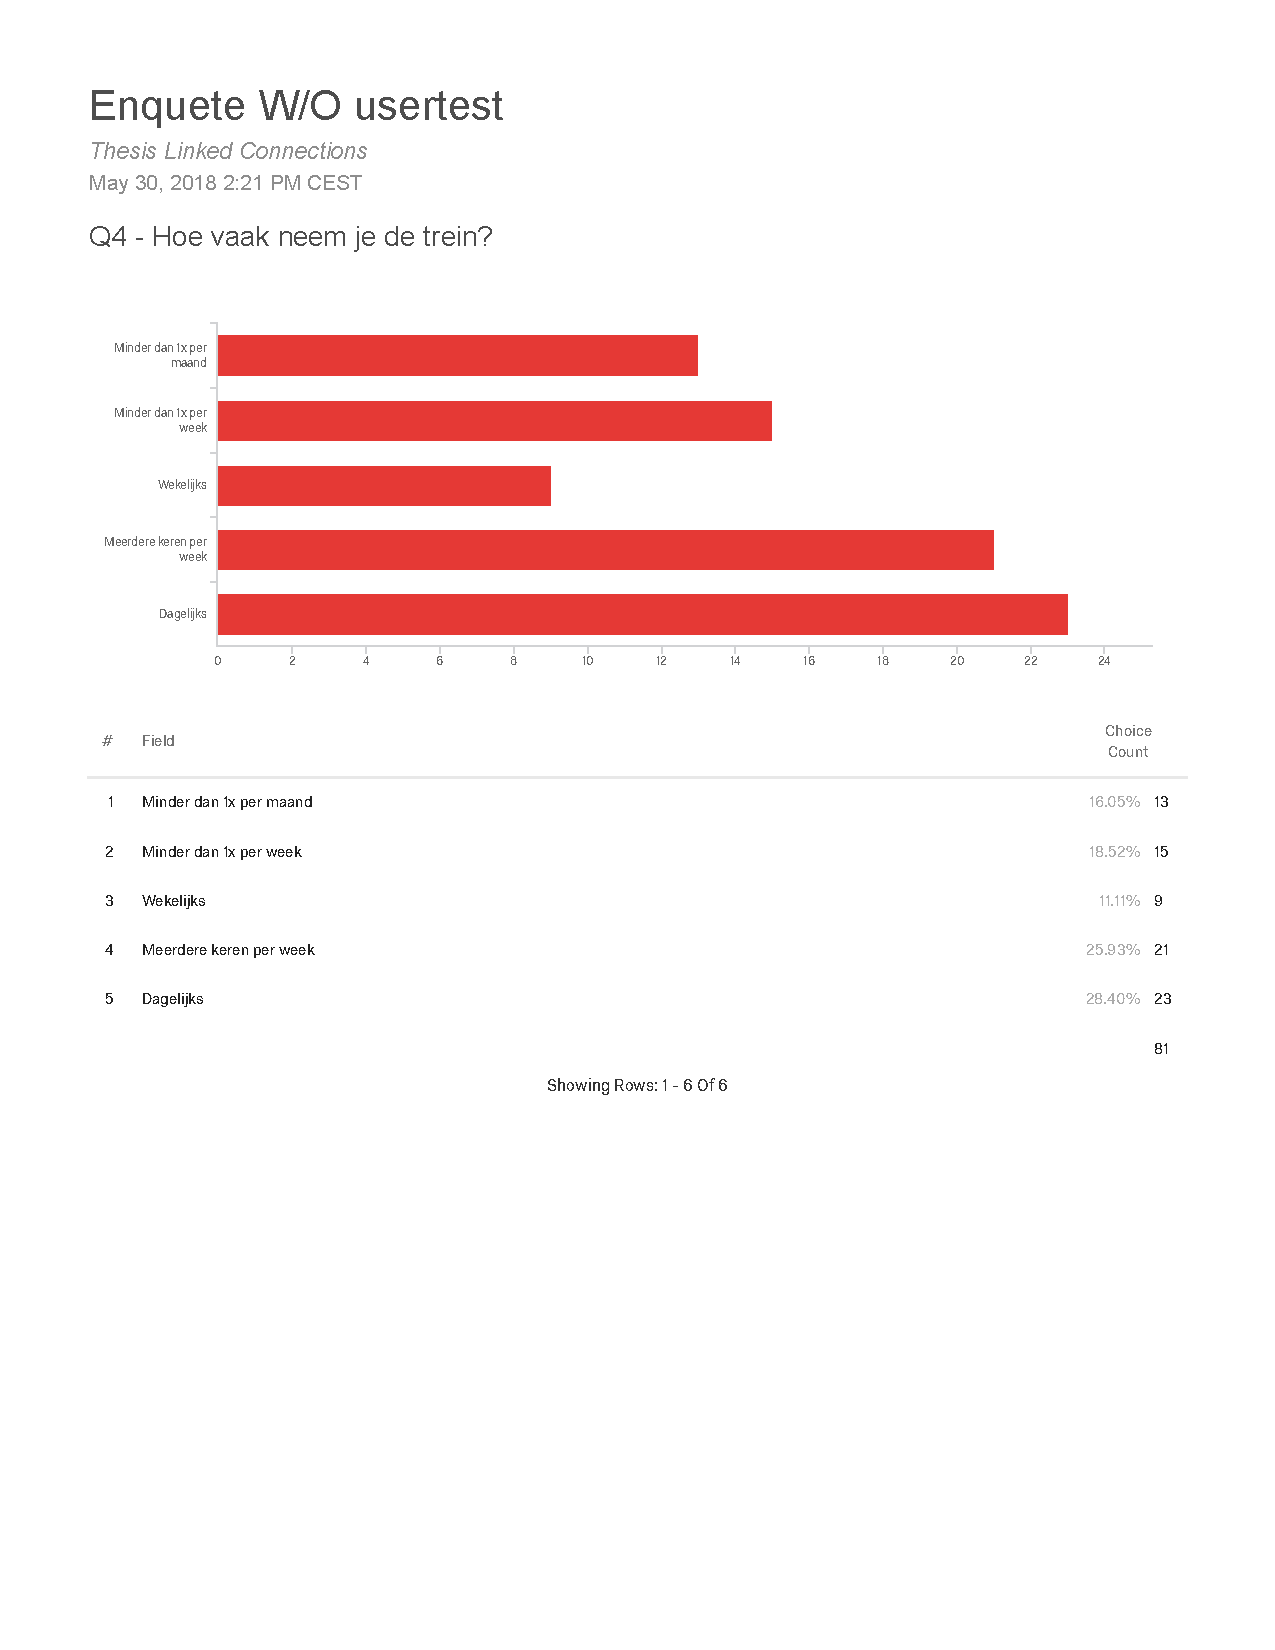
\includepdf[pages=-]{surveyreport.pdf}

\end{appendices}

\end{document}
